\documentclass[a4paper,12pt, twoside]{report}
\usepackage[utf8]{inputenc}
\usepackage[spanish]{babel}
\usepackage{amsmath}
\usepackage{makecell}
\usepackage{amsfonts}
\usepackage{amssymb}
\usepackage{multirow}
%\usepackage{makeidx}
\usepackage{graphicx}
\usepackage{fancyhdr}\pagestyle{fancy}
    \fancyhf{}
    \fancyhead[LO]{\it{\nouppercase{\leftmark}}}
    \fancyhead[RE]{\it{\nouppercase{\rightmark}}}
    \fancyhead[LE,RO]{\thepage}

    
\usepackage[usegeometry]{typearea}
\newenvironment{uselscape}{%
    \clearpage
    \KOMAoptions{paper=landscape, DIV=current}
    \newgeometry{top=2.5cm, left=3.2cm, right=2.5cm, bottom=2.5cm}
    \fancyheadoffset{0\linewidth}
}{%
    \clearpage
    \KOMAoptions{paper=portrait, DIV=current}
    \restoregeometry
}

\usepackage{hyperref}
\usepackage{float}
\usepackage{enumerate}
\usepackage[toc,page]{appendix}
\usepackage[nottoc]{tocbibind}
\usepackage{color}
\usepackage[dvipsnames]{xcolor}
\usepackage{tabularx}
\usepackage{pdflscape}
\usepackage{rotating}

\definecolor{gray97}{gray}{.97}
\definecolor{gray75}{gray}{.75}
\definecolor{gray45}{gray}{.45}
\usepackage{listings}
\lstset{ frame=Ltb,
     framerule=0pt,
     aboveskip=0.5cm,
     framextopmargin=3pt,
     framexbottommargin=3pt,
     framexleftmargin=0.4cm,
     framesep=0pt,
     rulesep=.4pt,
     backgroundcolor=\color{gray97},
     rulesepcolor=\color{black},
     %
     stringstyle=\ttfamily,
     showstringspaces = false,
     basicstyle=\small\ttfamily,
     commentstyle=\color{gray45},
     keywordstyle=\bfseries,
     %
     numbers=left,
     numbersep=15pt,
     numberstyle=\tiny,
     numberfirstline = false,
     breaklines=true,
   }
 
% minimizar fragmentado de listados
\lstnewenvironment{listing}[1][]
   {\lstset{#1}\pagebreak[0]}{\pagebreak[0]}
 
\lstdefinestyle{consola}
   {basicstyle=\scriptsize\bf\ttfamily,
    backgroundcolor=\color{gray75},
   }
 
\lstdefinestyle{C}
   {language=C,
   }
\usepackage[top=2.5cm, left=3.2cm, right=2.5cm, bottom=2.5cm]{geometry}
\pretolerance=2000
\tolerance=3000
\begin{document}

\begin{titlepage}
\begin{sffamily}
\color{NavyBlue}
\begin{center}
%\vspace*{-1cm}
\begin{figure}[htb]
\begin{center}
\vspace*{0.6cm}

\includegraphics[width=15cm]{figures/logoEHU_blanco_mediano.eps}
\vspace*{1.6cm}
\end{center}
\end{figure}
\begin{LARGE}
Máster Universitario en Modelización e Investigación Matemática, Estadística y Computación 
2023/2024 \\%indicar el curso académico
\vspace*{1cm}
\textsl{Trabajo Fin de Máster}\\
\end{LARGE}
\Huge{\textbf{Deep Reinforcement Learning en Trading Algorítmico: Una aplicación basada en ''Advances in Financial Machine Learning''}} %Más significativo que el anterior
\vspace*{1cm}
\rule{80mm}{0.1mm}\\
\huge{Alexander de la Puente González}\\ %Separar cada autor con \\ 
\vspace*{0.5cm}
\begin{Large}
Director/es\\
Josu Doncel Vicente\\
Leioa, 6 de Septiembre de 2024\\
\end{Large}
\end{center}
\end{sffamily}
\end{titlepage}

%\frontmatter
% \pagestyle{fancy}
% \fancyhead{} % Clear all header fields
% \setlength\headheight{21.2pt}
% \rhead{\color{NavyBlue} Mi encabezado} %Poner encabezado

\renewcommand{\tablename}{\textbf{Tabla}} %para poner la palabra en mayusucula
\renewcommand{\figurename}{\textbf{Figura}} % para poner la palabra en mayuscula
\renewcommand{\listtablename}{Índice de tablas}

\title{}
\date{}
\maketitle


\clearpage
\pagenumbering{Roman}
\setcounter{page}{1}

\tableofcontents
%\thispagestyle{empty}

\listoffigures
%\thispagestyle{empty}

\listoftables
%\thispagestyle{empty}

%Para imagenes
%\begin{figure}[H]
%\centering
%\includegraphics[scale=0.8]{imagenes/*.png}
%\caption{}
%\end{figure}

%\mainmatter
\clearpage
\pagenumbering{arabic}
\setcounter{page}{1}

%Comenzar el trabajo

\chapter{Introducción}

El trading financiero es un campo en constante evolución, impulsado por los avances tecnológicos 
y el creciente uso de técnicas de \textit{machine learning} y \textit{deep learning}. Entre estas, 
el \textit{deep reinforcement learning} se ha destacado como una metodología prometedora para 
desarrollar estrategias de trading que pueden adaptarse dinámicamente a las condiciones cambiantes 
del mercado. Este proyecto surge de una motivación personal y académica de explorar y aprender a 
desarrollar estrategias de trading utilizando técnicas avanzadas de \textit{machine learning}.

Una de las principales motivaciones de este trabajo es aprender a implementar un agente de 
\textit{deep reinforcement learning} para la creación de estrategias de trading. Con el auge 
de las librerías gratuitas como \textit{Gymnasium} y \textit{Stable Baselines}, se abre una 
oportunidad única para aprender y aplicar estas herramientas en el diseño, entrenamiento y evaluación 
de agentes de aprendizaje por refuerzo. Además, este proyecto busca profundizar en las metodologías 
propuestas en el libro \textit{Advances in Financial Machine Learning} de Marcos López de Prado, 
un referente en la aplicación de técnicas de \textit{machine learning} al análisis financiero. 
La implementación y evaluación de estas metodologías permitirán no solo entender mejor cómo 
funcionan, sino también cómo pueden ayudar en la creación de estrategias de trading más robustas 
y efectivas.

Otro aspecto clave de esta investigación es evaluar la accesibilidad y aplicabilidad de estas 
técnicas para personas que no provienen del ámbito financiero. A medida que el trading algorítmico 
y las técnicas de \textit{machine learning} se vuelven más comunes, es crucial entender cómo alguien 
con un trasfondo técnico, pero sin experiencia directa en finanzas, puede acercarse a esta disciplina. 
El objetivo es identificar las barreras de entrada, los desafíos y las oportunidades que presenta 
este campo, así como evaluar qué tan cerca o lejos está esta disciplina de ser accesible para un 
público más amplio.

En resumen, este trabajo tiene como objetivo aprender y aplicar técnicas avanzadas de 
\textit{machine learning}, específicamente \textit{deep reinforcement learning}, en el desarrollo 
de estrategias de trading, utilizando herramientas accesibles y metodologías de vanguardia. A través 
de este proceso, se pretende obtener una comprensión más profunda del potencial y las limitaciones 
de estas técnicas en un contexto financiero, contribuyendo así al conocimiento en esta intersección 
entre tecnología y finanzas.


\section{Contextualización del problema}

El desarrollo de estrategias de trading efectivas en un entorno financiero altamente dinámico 
requiere la implementación de técnicas avanzadas que puedan adaptarse a las complejidades y 
variabilidades del mercado. En este trabajo, se plantea una estrategia integral que combina 
varias metodologías innovadoras con el objetivo de evaluar su utilidad en la generación de 
estrategias de trading robustas y efectivas.

El primer componente clave de esta estrategia es la implementación de barras de desequilibrio 
de volumen y dólares, una técnica que ofrece una representación más precisa de la actividad 
del mercado en comparación con las barras de tiempo tradicionales. Estas barras se 
construyen basándose en la actividad real del mercado, en lugar de intervalos de tiempo fijos, 
lo que permite capturar mejor la dinámica subyacente de la oferta y la demanda. Este enfoque 
se evaluará en conjunto con las barras de tiempo convencionales para determinar si proporcionan 
una ventaja en la formación de estrategias de trading.

El segundo componente es el entrenamiento de un algoritmo de \textit{deep reinforcement learning} 
(DRL) sobre estas barras construidas y sobre las barras originales. El objetivo aquí es explorar 
cómo las diferentes representaciones del mercado afectan el rendimiento del algoritmo de DRL 
en la identificación de oportunidades de trading. Este enfoque permitirá no solo evaluar la 
efectividad del aprendizaje por refuerzo en estos distintos contextos, sino también determinar 
si la precisión y la estabilidad del agente de trading pueden mejorar al cambiar la base de 
datos sobre la que se entrena.

Finalmente, se aplicará la técnica de \textit{Meta-Labeling} sobre las señales generadas 
por el algoritmo de \textit{deep reinforcement learning}. El \textit{Meta-Labeling} actúa 
como una capa adicional de análisis, refinando las señales emitidas y potenciando la capacidad 
del modelo para filtrar las señales más prometedoras. La efectividad de esta técnica se evaluará 
comparando su rendimiento con el de las señales originales, así como con otros enfoques sin 
\textit{Meta-Labeling}.

El planteamiento de esta estrategia no solo busca implementar y analizar cada una de estas 
técnicas de manera individual, sino también explorar cómo funcionan en conjunto. Se realizará 
una comparativa exhaustiva entre las diferentes configuraciones para determinar cuáles ofrecen 
los mejores resultados en términos de precisión, estabilidad y rentabilidad en las estrategias 
de trading. Este enfoque permitirá obtener una visión más completa de cómo estas técnicas 
pueden contribuir al desarrollo de modelos de trading más eficaces y adaptativos.


% \section{Antecedentes}

% Diversos estudios y trabajos han explorado la aplicación de RL en finanzas. Por ejemplo, Dindos y Pipher (\cite{DindosPipherRule2016}) 
% demostraron la viabilidad de usar RL para optimizar portafolios financieros. Además, López de Prado en su libro 
% "Advances in Financial Machine Learning" proporciona una guía exhaustiva sobre técnicas avanzadas de machine learning aplicadas a finanzas, 
% que sirven como base para este trabajo.


\section{Estructura del Documento}

Este documento se organiza en siete capítulos, cada uno de los cuales aborda un aspecto clave del desarrollo de estrategias de trading utilizando técnicas avanzadas de \textit{machine learning}:

\begin{itemize}
    \item \textbf{Capítulo 1: Introducción.} Se presenta la motivación, los objetivos del trabajo y una contextualización inicial del planteamiento de la estrategia.

    \item \textbf{Capítulo 2: Fundamentos de los Datos Financieros.} En este capítulo se introducen los conceptos financieros relevantes que son fundamentales para comprender los datos utilizados en las estrategias de trading. Se abordan temas como la naturaleza de los datos financieros, tipos de barras, y la importancia de la estructura de los datos en el análisis y la toma de decisiones.

    \item \textbf{Capítulo 3: Barras de Desequilibrio.} Este capítulo explora la implementación de barras de desequilibrio de volumen y dólares como una alternativa a las barras de tiempo tradicionales. Se discuten sus ventajas, su construcción y su impacto en la precisión del análisis de mercado.

    \item \textbf{Capítulo 4: Aprendizaje por Refuerzo.} Aquí se detalla el uso del \textit{deep reinforcement learning} para entrenar agentes de trading sobre las barras de desequilibrio y las barras de tiempo originales. Se analizan las técnicas y algoritmos utilizados, así como los resultados esperados de estos enfoques.

    \item \textbf{Capítulo 5: Meta-Labeling.} En este capítulo se profundiza en la técnica de \textit{Meta-Labeling}, su implementación sobre las señales generadas por los modelos de aprendizaje por refuerzo, y cómo esta técnica puede mejorar la precisión y la gestión del riesgo en las estrategias de trading.

    \item \textbf{Capítulo 6: Resultados.} Se presentan los resultados obtenidos de las implementaciones y evaluaciones realizadas en los capítulos anteriores. Se comparan las diferentes técnicas utilizadas y se discuten sus ventajas y limitaciones.

    \item \textbf{Capítulo 7: Conclusiones.} En el capítulo final se resumen los hallazgos clave del trabajo, se destacan las principales contribuciones, y se proponen posibles líneas de investigación futura para continuar explorando y mejorando las estrategias de trading basadas en \textit{machine learning}.
\end{itemize}

Esta estructura proporciona una visión clara y coherente del flujo del trabajo, desde la introducción de conceptos fundamentales hasta la implementación y evaluación de técnicas avanzadas, culminando en las conclusiones sobre su efectividad y aplicabilidad.


\chapter{Fundamentos de los datos Financieros}
\section{Descripción de los Datos Financieros}

Aunque los datos financieros vienen en muchas formas, este trabajo se centrará en aquellos provenientes de acciones o índices 
(cestas de instrumentos financieros). Para simplificar, en lugar de pensar en instrumentos financieros individuales, consideraremos 
la serie temporal subyacente de precios.

\subsection{Introducción a la Serie Temporal}

La serie temporal $\{p_t\}$ representa el precio de una acción o índice en el instante de tiempo discreto $t$. Es importante 
notar que $t$ dependerá de la frecuencia de muestreo utilizada para recopilar los datos.

\subsubsection{Frecuencia}

\begin{itemize}
    \item \textbf{Datos de Baja Frecuencia (LF)}: Diarios, mensuales, trimestrales.
    \item \textbf{Datos de Alta Frecuencia (HF)}: Intradía (30 min., 5 min., etc.).
\end{itemize}

Al introducir estos conceptos, es pertinente señalar que el modelado en finanzas se realiza con el logaritmo natural del precio 
(log-precios) en lugar de los precios regulares. Esto se representará como $y_t := \log(p_t)$. Para ilustrar esto, se 
introduce el simple, pero ampliamente utilizado, modelo de un paseo aleatorio con deriva:

\begin{equation}
y_t = y_{t-1} + \mu + \epsilon_t,
\end{equation}

En esta ecuación, $\mu$ representa la \textit{deriva}, que indica la tendencia media 
del logaritmo del precio a lo largo del tiempo. Un valor positivo de $\mu$ implica un 
crecimiento promedio en los precios, mientras que un valor negativo refleja una tendencia decreciente. 

Por otro lado, $\epsilon_t$ es el \textit{término de ruido} o \textit{error aleatorio}, que captura 
las fluctuaciones impredecibles en el precio. Generalmente, se asume que $\epsilon_t$ es 
una variable aleatoria con media cero y varianza constante, lo que refleja la naturaleza 
estocástica del proceso de formación de precios.


%% donde $\epsilon_t \sim i.i.d. \mathcal{N}(0, \sigma^2)$.

\subsection{Retornos de Activos}

El siguiente concepto a introducir son los retornos, una técnica para normalizar los precios y permitir la comparación 
entre diferentes series temporales, independientemente del valor del precio. Los dos tipos que se van a utilizar son 
los retornos lineales y logarítmicos.

\begin{itemize}
    \item \textbf{Lineales}: $R_t := \frac{p_t - p_{t-1}}{p_{t-1}} = \frac{p_t}{p_{t-1}} - 1$
    \item \textbf{Logarítmicos}: $r_t := \log\left(\frac{p_t}{p_{t-1}}\right) = \log(p_t) - \log(p_{t-1}) = y_t - y_{t-1}$
\end{itemize}

\begin{figure}[H]
    \centering
    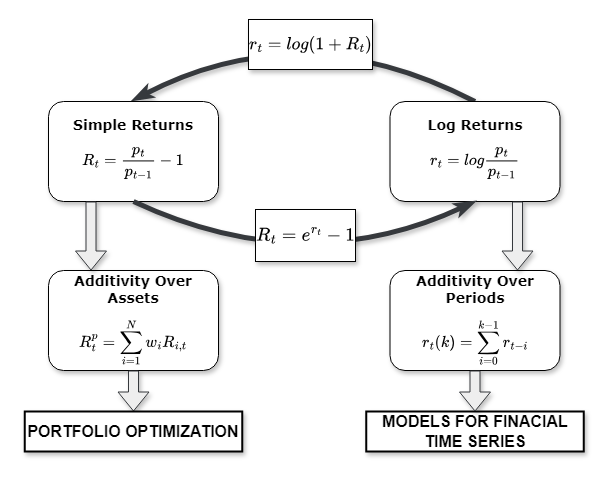
\includegraphics[width=0.8\textwidth]{figures/simple_and_log_ret_relation.png}
    \caption{Relación entre retornos simples y logarítmicos, adaptación de \cite{signal_processing}}
    \label{fig:log-returns}
\end{figure}

La figura \ref{fig:log-returns} muestra la relación existente entre los retornos logarítmicos y los retornos simples.
Ambos serán utilizados a lo largo de este trabajo tanto para el entrenamiento del agente de aprendizaje por refuerzo en
como para el cálculo de los rendimientos generados por las estratégias construídas.

\section{Hechos Estilizados}

Los hechos estilizados son patrones o regularidades observadas empíricamente en los datos financieros que se 
presentan de manera consistente en diferentes mercados, periodos de tiempo y condiciones económicas. Estos hechos 
no dependen de modelos teóricos específicos, sino que se derivan directamente de la observación de los datos. La 
identificación de estos patrones es crucial para el desarrollo y validación de modelos financieros y econométricos. 
En este trabajo, nos basamos en los hechos estilizados descritos por Rama Cont (2001) en su artículo \textit{Empirical 
properties of asset returns: stylized facts and statistical issues} \cite{Cont2001}.

A continuación, se describen los principales hechos estilizados relevantes para este estudio:

\begin{enumerate}
    \item \textbf{Ausencia de Autocorrelaciones}: Los retornos de los activos financieros, especialmente en 
    frecuencias diarias y superiores, tienden a mostrar una autocorrelación lineal insignificante. Esto significa 
    que los retornos pasados no son buenos predictores de los retornos futuros, lo cual es consistente con la hipótesis 
    del mercado eficiente en su forma débil. Sin embargo, en escalas temporales intradía, pueden observarse autocorrelaciones significativas.
    \item \textbf{Colas Pesadas}: La distribución de los retornos de los activos financieros presenta colas más gruesas que una distribución 
    normal. Esto implica que los eventos extremos (grandes movimientos de precios) ocurren con mayor frecuencia de lo que se esperaría bajo 
    una distribución normal. Las colas pesadas se modelan mejor con distribuciones como la distribución de Pareto o la distribución t de Student.
    \item \textbf{Asimetría de Ganancias/Pérdidas}: Los retornos de los activos financieros muestran una asimetría en sus movimientos extremos. 
    Las caídas bruscas en los precios (pérdidas) son más comunes y pronunciadas que los incrementos bruscos (ganancias). Esto se debe a factores 
    como el pánico de los inversores y las ventas masivas en respuesta a malas noticias.
    \item \textbf{Gaussianidad Agregada}: A medida que se incrementa la escala temporal sobre la cual se calculan los retornos (por ejemplo, 
    pasando de retornos diarios a retornos mensuales), la distribución de los retornos tiende a aproximarse a una distribución normal. Esto es 
    consistente con el teorema central del límite, que establece que la suma de variables aleatorias independientes y con varianza finita tiende 
    hacia una distribución normal.
    \item \textbf{Intermitencia}: Los retornos financieros muestran una alta variabilidad en todas las escalas temporales. Esto significa que 
    los periodos de alta y baja volatilidad no están distribuidos uniformemente en el tiempo, sino que se alternan de manera impredecible.
    \item \textbf{Agrupamiento de Volatilidad}: La volatilidad de los retornos tiende a aparecer en clústeres. Periodos de alta volatilidad 
    tienden a ser seguidos por más periodos de alta volatilidad, y lo mismo ocurre con los periodos de baja volatilidad. Este fenómeno se 
    puede modelar mediante modelos de heterocedasticidad condicional, como los modelos GARCH (Generalized Autoregressive Conditional 
    Heteroskedasticity).
\end{enumerate}

Estos hechos estilizados proporcionan una base empírica sobre la cual se pueden construir y validar modelos financieros. La identificación 
y comprensión de estos patrones ayudan a mejorar la precisión de los modelos de riesgo, a desarrollar estrategias de trading más robustas 
y a diseñar mejores políticas de regulación financiera.


\subsection{Datos de Alta Frecuencia}

Los datos de alta frecuencia (HF) representan el registro de precios y volúmenes de transacciones de activos financieros en intervalos 
de tiempo muy cortos, como segundos o milisegundos. Estos datos incluyen información detallada sobre cada transacción, como el precio, 
la cantidad negociada y el tiempo exacto de la transacción. A continuación, se detallan algunas características clave de los datos de 
alta frecuencia:

\begin{itemize}
    \item \textbf{Granularidad Temporal}: Los datos se registran en intervalos muy cortos, lo que permite un análisis detallado de la 
    dinámica del mercado en el corto plazo.
    \item \textbf{Volumen de Datos}: La gran cantidad de transacciones que ocurren en cortos periodos de tiempo genera volúmenes 
    masivos de datos que deben ser almacenados y procesados.
    \item \textbf{Precisión}: Incluyen información precisa sobre el precio y el volumen de cada transacción, así como el tiempo exacto 
    en que ocurrieron.
    \item \textbf{Eventos de Mercado}: Los datos de alta frecuencia capturan eventos de mercado que no son visibles en datos de menor 
    frecuencia, como órdenes de compra y venta, cambios en la profundidad del mercado y reacciones instantáneas a noticias.
\end{itemize}

A pesar de sus ventajas, los datos de alta frecuencia presentan varios desafíos:

\begin{itemize}
    \item \textbf{Costo y Accesibilidad}: Los datos de alta frecuencia son difíciles y costosos de obtener, ya que generalmente requieren 
    suscripciones a servicios de datos financieros especializados y costosos.
    \item \textbf{Procesamiento y Almacenamiento}: El volumen masivo de datos requiere infraestructuras avanzadas para su almacenamiento 
    y procesamiento eficiente.
    \item \textbf{Ruido y Volatilidad}: La alta granularidad temporal de estos datos incluye mucho ruido, lo que puede complicar el 
    análisis y modelado.
\end{itemize}

Debido a estos desafíos, en este trabajo se utilizarán datos de minuto. Los datos de minuto representan un compromiso entre la 
granularidad y la manejabilidad, proporcionando suficiente detalle para un análisis robusto sin los costos y complejidades asociados 
con los datos de alta frecuencia. Estos datos son más accesibles y permiten capturar las tendencias y patrones intradía sin la 
sobrecarga de procesamiento asociada con datos de mayor frecuencia.

% \begin{figure}[H]
%     \centering
%     \includegraphics[width=0.8\textwidth]{minute_data_example.png}
%     \caption{Ejemplo de Datos de Minuto}
%     \label{fig:minute-data-example}
% \end{figure}


\subsection{Datos Utilizados}


En este trabajo se utilizarán dos conjuntos de datos financieros: los datos de Bitcoin y los 
datos del SPY (SPDR S\&P 500 ETF Trust).

El S\&P 500 es un índice que agrupa a las 500 de mayor capitalización 
de Estados Unidos. Este índice es utilizado como referencia del rendimiento 
del mercado bursátil estadounidense debido a su diversificación y su capacidad 
para reflejar el estado general de la economía. Sin embargo, no es posible invertir 
directamente en un índice, lo que lleva a los inversores a optar por el SPY, 
un \textit{Exchange Traded Fund} (ETF) que replica el comportamiento del 
S\&P 500.

Un \textit{Exchange Traded Fund} (ETF) es un fondo que replica el rendimiento de un 
conjunto de activos y se negocia en bolsa como si fuera una acción. Un ejemplo claro 
es el SPY, que es un ETF diseñado para seguir el comportamiento del índice S\&P 500. 
Esto significa que cuando un inversor compra una participación en el SPY, está 
adquiriendo una porción de todas las empresas que componen el S\&P 500, lo que lo 
convierte en una alternativa práctica y accesible para replicar el rendimiento 
del índice.

En cuanto al Bitcoin, es una criptomoneda descentralizada que se basa en la tecnología 
blockchain. A diferencia de las monedas tradicionales, no está respaldada por ningún 
gobierno o institución financiera. Su creación y gestión se realizan mediante un 
sistema de código abierto, donde las transacciones se verifican a través de una red 
descentralizada de nodos que utilizan un protocolo de consenso conocido como 
\textit{Proof of Work} (Prueba de Trabajo).

Bitcoin se ha convertido en un activo popular tanto para inversión como para su uso 
como medio de intercambio y es considerado por muchos como una reserva de valor 
y una alternativa a las monedas tradicionales. Al igual que los ETF, puede negociarse 
en mercados, aunque su volatilidad y falta de regulación presentan riesgos 
adicionales para los inversores.



Ambas series temporales cubren el período desde el 
1 de enero de 2018 hasta el 30 de junio de 2024. La división de los datos se realizará de la 
siguiente manera: el conjunto de datos in-sample abarcará desde el inicio de la serie hasta 
el 31 de diciembre de 2022, mientras que el conjunto de datos out-of-sample cubrirá desde el 
1 de enero de 2023 hasta el final del periodo.

El conjunto in-sample se utiliza para entrenar los modelos de aprendizaje automático, 
ajustando los parámetros y calibrando el rendimiento del agente de aprendizaje por refuerzo. 
Por otro lado, el conjunto out-of-sample sirve para evaluar la generalización del modelo a 
nuevos datos que no fueron utilizados durante el entrenamiento, proporcionando así una 
estimación más precisa del rendimiento real del modelo en escenarios futuros. Esta separación 
es fundamental en inteligencia artificial y machine learning para evitar el sobreajuste y 
asegurar que el modelo sea robusto y capaz de adaptarse a variaciones en los datos.

\begin{figure}[H]
    \centering
    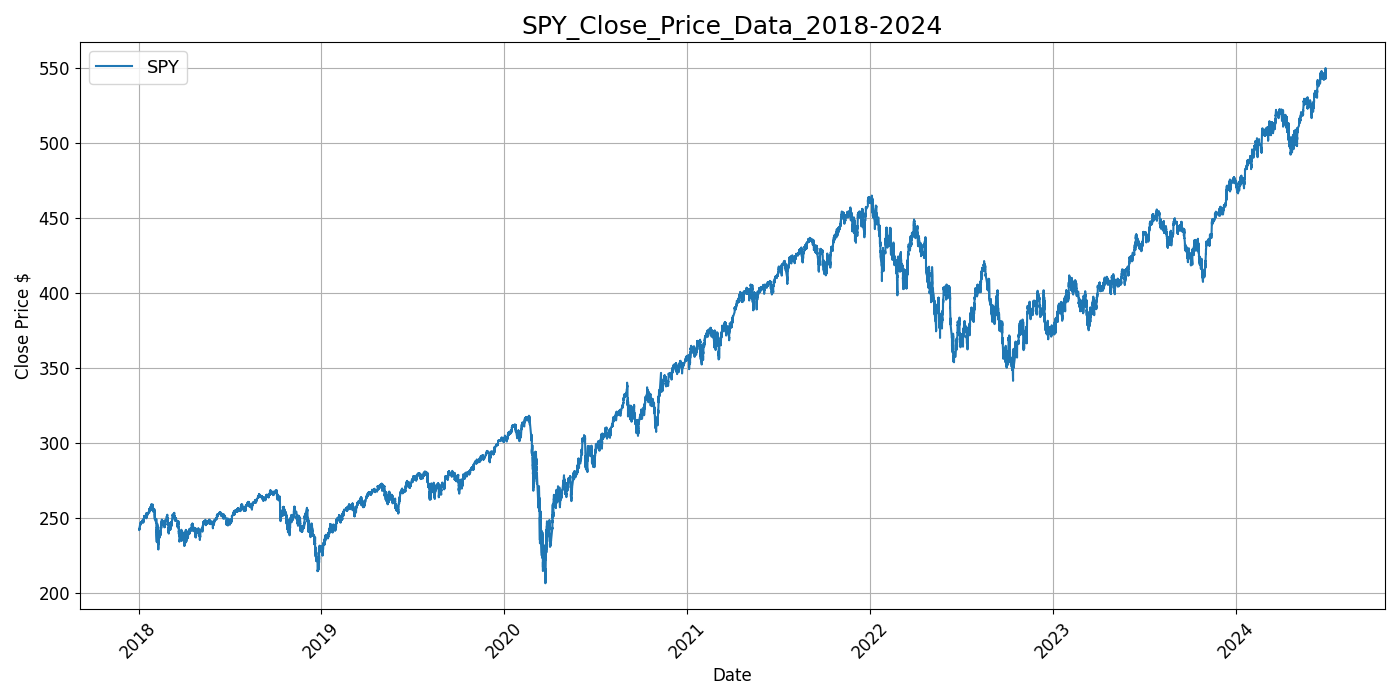
\includegraphics[width=0.8\textwidth]{figures/SPY_Close_Price_Data_2018-2024.png}
    \caption{Serie Temporal de Precios del SPY}
    \label{fig:spy-prices}
\end{figure}

Las Figuras \ref{fig:spy-prices} y \ref{fig:bitcoin-prices} muestran las series temporales de ambos activos: 
de Bitcoin:

\begin{figure}[H]
    \centering
    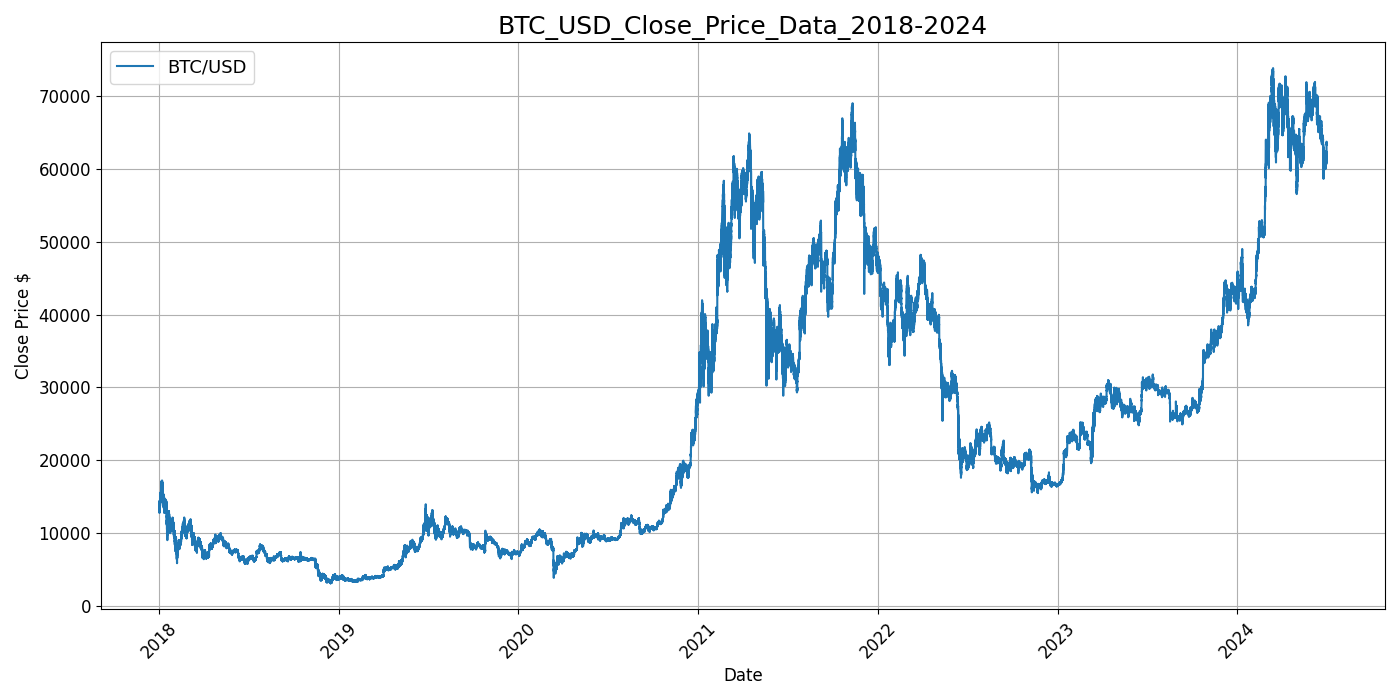
\includegraphics[width=0.8\textwidth]{./figures/BTC_USD_Close_Price_Data_2018-2024.png}
    \caption{Serie Temporal de Precios de Bitcoin}
    \label{fig:bitcoin-prices}
\end{figure}


\section{Métricas Financieras}

Para evaluar el rendimiento de una estrategia de trading, es crucial utilizar métricas financieras adecuadas que permitan comparar y analizar los resultados obtenidos. A continuación, se describen algunas de las métricas financieras más utilizadas junto con sus expresiones matemáticas.

\subsubsection{Cumulative Returns}

Los \textit{Cumulative Returns} (\textit{Retornos Acumulados}) representan el total de los retornos obtenidos por una inversión desde el inicio hasta un punto en el tiempo. Se calculan como el producto de los rendimientos individuales de cada período.

\begin{equation}
\text{Cumulative Returns} = \prod_{i=1}^{n} (1 + r_i) - 1,
\end{equation}

donde $r_i$ es el retorno en el período $i$.

\subsubsection{Annualized Return}

El \textit{Annualized Return} (\textit{Retorno Anualizado}) mide el rendimiento medio anual de una inversión, ajustando el rendimiento acumulado para que se exprese en una base anual.

\begin{equation}
\text{Annualized Return} = \left(1 + \text{Cumulative Returns}\right)^{\frac{1}{T}} - 1,
\end{equation}

donde $T$ es el número de años.

\subsubsection{Sharpe Ratio}

El \textit{Sharpe Ratio} \cite{sharpe1994}, desarrollado por William F. Sharpe en 1966 y revisado 
posteriormente en 1994, es una medida que evalúa el rendimiento ajustado al riesgo de una inversión. 
Compara el exceso de retorno de una cartera sobre la tasa libre de riesgo con la volatilidad de esos 
retornos. Este ratio es ampliamente utilizado en la gestión de portafolios y finanzas cuantitativas, 
ya que permite a los inversores evaluar si los rendimientos obtenidos compensan adecuadamente el 
riesgo asumido.

Sharpe introdujo esta medida como una herramienta para comparar inversiones con diferentes 
niveles de riesgo, permitiendo una mejor toma de decisiones en la optimización de carteras.

\begin{equation}
\text{Sharpe Ratio} = \frac{E[R_p - R_f]}{\sigma_p},
\end{equation}

donde $R_p$ es el retorno de la cartera, $R_f$ es la tasa libre de riesgo, y $\sigma_p$ es 
la desviación estándar de los retornos de la cartera. Un Sharpe Ratio más alto indica que la 
inversión ha generado un retorno mayor por cada unidad de riesgo asumido.

\subsubsection{Sortino Ratio}


El \textit{Sortino Ratio} \cite{sortino1994}, desarrollado por Frank A. Sortino en 1994, es una adaptación 
del Sharpe Ratio que tiene en cuenta únicamente la volatilidad de los retornos negativos, o 
\textit{downside risk}, ofreciendo así una visión más precisa del rendimiento ajustado al riesgo. 
A diferencia del Sharpe Ratio, que penaliza tanto las subidas como las bajadas de la misma manera, 
el Sortino Ratio solo castiga los retornos por debajo de un umbral predefinido, lo que es especialmente 
útil para los inversores que desean minimizar las pérdidas.

Sortino introdujo este ratio en su trabajo "Performance Measurement in a Downside Risk Framework", donde 
argumenta que la verdadera preocupación de los inversores no es la volatilidad general, sino las pérdidas. 
Este ratio es especialmente útil para evaluar estrategias de inversión que buscan limitar la volatilidad negativa, 
recompensando las carteras con una mayor asimetría positiva (retornos altos y bajas pérdidas).

\begin{equation}
\text{Sortino Ratio} = \frac{E[R_p - R_f]}{\sigma_{d}},
\end{equation}

donde $\sigma_{d}$ es la desviación estándar de los retornos negativos. Un Sortino Ratio más alto 
indica que la inversión está generando un mayor retorno ajustado al riesgo al penalizar únicamente 
los movimientos negativos, lo que lo convierte en una herramienta esencial para los gestores de 
carteras que buscan minimizar el riesgo a la baja.

\subsubsection{Maximum Drawdown}

El \textit{Maximum Drawdown} (\textit{Máxima Pérdida}) mide la mayor caída en el valor de una cartera desde un máximo anterior hasta un mínimo posterior, lo que indica el peor comportamiento de la estrategia en términos de pérdida de valor.

\begin{equation}
\text{Maximum Drawdown} = \min_{t \in [0,T]} \left(\frac{V_t - V_{\text{max}, t}}{V_{\text{max}, t}}\right),
\end{equation}

donde $V_t$ es el valor de la cartera en el tiempo $t$, y $V_{\text{max}, t}$ es el valor máximo de la cartera hasta el tiempo $t$.

\subsubsection{Calmar Ratio}

El \textit{Calmar Ratio} mide el rendimiento ajustado al riesgo de una inversión, similar al Sharpe Ratio, pero utilizando el \textit{Maximum Drawdown} como medida del riesgo.

\begin{equation}
\text{Calmar Ratio} = \frac{\text{Annualized Return}}{\text{Maximum Drawdown}}.
\end{equation}

% \subsubsection{Value at Risk (VaR)}

% El \textit{Value at Risk} (\textit{VaR}) mide la pérdida máxima esperada de una inversión en un período determinado, con un nivel de confianza específico. Es una medida de riesgo que indica el valor en riesgo.

% \begin{equation}
% \text{VaR}_{\alpha} = -\text{Quantile}_\alpha (R_p),
% \end{equation}

% donde $\alpha$ es el nivel de confianza y $R_p$ es la distribución de retornos de la cartera.

\subsubsection{Alpha}

El \textit{Alpha} mide el rendimiento adicional que una inversión genera en comparación con su benchmark, ajustado por el riesgo. Es un indicador de la habilidad del gestor de la cartera para generar rendimientos superiores.

\begin{equation}
\alpha = R_p - \left(R_f + \beta (R_m - R_f)\right),
\end{equation}

donde $R_m$ es el retorno del mercado, y $\beta$ es la sensibilidad de la cartera al mercado.

\subsubsection{Beta}

El \textit{Beta} mide la sensibilidad de los retornos de una cartera en relación con los movimientos del mercado. Un $\beta$ mayor que 1 indica que la cartera es más volátil que el mercado.

\begin{equation}
\beta = \frac{\text{Cov}(R_p, R_m)}{\sigma^2_m},
\end{equation}

donde $\text{Cov}(R_p, R_m)$ es la covarianza entre los retornos de la cartera y los del mercado, y $\sigma^2_m$ es la varianza de los retornos del mercado.

\section{Métricas de Machine Learning}

Las métricas de evaluación son fundamentales para medir el rendimiento de los modelos de \textit{Machine Learning}, especialmente en el contexto de clasificación. A continuación, se describen algunas de las métricas más utilizadas en la evaluación de modelos de clasificación.

\subsubsection{Precision}

La \textit{Precision} (Precisión) mide la proporción de verdaderos positivos (TP) entre todas las predicciones positivas realizadas por el modelo. Es una medida de la exactitud del modelo cuando predice la clase positiva.

\begin{equation}
\text{Precision} = \frac{TP}{TP + FP},
\end{equation}

donde $TP$ son los verdaderos positivos y $FP$ son los falsos positivos.

\subsubsection{Recall}

El \textit{Recall} (Cobertura o Sensibilidad) mide la proporción de verdaderos positivos entre todos los ejemplos que realmente son positivos. Es una medida de la capacidad del modelo para identificar correctamente las instancias positivas.

\begin{equation}
\text{Recall} = \frac{TP}{TP + FN},
\end{equation}

donde $FN$ son los falsos negativos.

\subsubsection{F1-Score}

El \textit{F1-Score} es la media armónica de la \textit{Precision} y el \textit{Recall}, proporcionando un balance entre ambas métricas. Es especialmente útil cuando se desea tener un equilibrio entre la precisión y la cobertura.

\begin{equation}
\text{F1-Score} = \frac{2 \cdot \text{Precision} \cdot \text{Recall}}{\text{Precision} + \text{Recall}}.
\end{equation}


\chapter{Barras de desequilibrio}

\section{Barras Basadas en Información}

En la industria financiera, es común el uso de barras de tiempo para transformar 
series de observaciones que llegan a intervalos irregulares en series homogéneas 
derivadas de un muestreo regular. Las barras de tiempo, obtenidas al muestrear 
información en intervalos de tiempo fijos (por ejemplo, cada minuto), suelen incluir 
datos como la marca temporal, el precio de apertura, el precio de cierre, el precio 
más alto, el más bajo, y el volumen negociado. Estos datos se conocen como datos \textit{ohclv}.

Aunque las barras de tiempo son populares tanto entre los profesionales como entre los académicos, 
el libro de Marcos López de Prado introduce las limitaciones que presentan este tipo de datos:

\begin{itemize}
    \item Los mercados no procesan información a intervalos de tiempo constantes. Por ejemplo, la 
    actividad es significativamente mayor en las horas inmediatamente posteriores a la apertura, 
    en comparación con periodos de menor actividad, como el mediodía.
    \item Las barras de tiempo tienden a sobre-representar la actividad durante periodos tranquilos 
    y sub-representar durante momentos de alta actividad, lo que distorsiona la representatividad de los datos.
    \item Las series temporales basadas en tiempo suelen exhibir propiedades estadísticas deficientes, 
    como correlación serial, heteroscedasticidad y no-normalidad de los retornos, lo que complica el 
    modelado y análisis de los datos.
\end{itemize}

Formar barras basadas en la información de mercado, en lugar de intervalos de tiempo fijos, 
es una alternativa que mejora la representatividad de los datos y las propiedades estadísticas 
de las series temporales generadas. 

Este tipo de barras basadas en información ajustan dinámicamente el tamaño de las barras
en respuesta a la llegada de nueva información, lo que permite una representación
más precisa de las condiciones de mercado. Este enfoque es útil para identificar y reaccionar 
ante la presencia de traders
informados, quienes pueden provocar desequilibrios en los precios.

\subsection{Barras de Desequilibrio}

Las barras de desequilibrio son un tipo de barra basada en información que ajusta el muestreo 
según la actividad del mercado en lugar de hacerlo a intervalos de tiempo fijos. Este enfoque 
permite capturar de manera más efectiva los momentos en que se produce nueva información relevante, 
mejorando así la capacidad de respuesta ante los cambios del mercado.

\subsubsection{La Regla del Tick}

En el ámbito de la microestructura del mercado, es esencial comprender cómo se generan y clasifican las operaciones. En un 
libro de órdenes de subasta doble, se registran cotizaciones para vender (ofertas) y comprar (demandas) un valor a diferentes 
niveles de precios. Las operaciones ocurren cuando un comprador coincide con una oferta o un vendedor con una demanda. La regla 
del tick es una herramienta que permite identificar el lado agresor de cada operación. Esta regla clasifica una transacción 
como iniciada por el comprador si el precio sube (\(\Delta p_t > 0\)) o por el vendedor si el precio baja (\(\Delta p_t < 0\)). 
Si el precio se mantiene igual (\(\Delta p_t = 0\)), la clasificación se mantiene según el último tick registrado:

\begin{equation}
b_t =
\begin{cases}
1 & \text{si} \ \Delta p_t > 0 \\
-1 & \text{si} \ \Delta p_t < 0 \\
b_{t-1} & \text{si} \ \Delta p_t = 0
\end{cases},
\end{equation}

donde \(p_t\) es el precio de la operación indexado por \(t = 1,\ldots,T\) y \(b_0\) se establece arbitrariamente en 1. 
La regla del tick, a pesar de su simplicidad, ha demostrado ser efectiva en la clasificación de transacciones, con una 
alta precisión documentada en varios estudios \cite{aitken1996accuracy}.

\subsubsection{Tipos de Barras de Desequilibrio}

\paragraph{Barras de Desequilibrio de Tick (TIB)}

Las barras de desequilibrio de tick se basan en la idea de que el desequilibrio en los ticks puede revelar información 
importante. Se consideran secuencias de ticks donde cada tick tiene un precio \(p_t\) y un volumen \(v_t\). La regla del tick 
se utiliza para generar una secuencia \(\{b_t\}\) que clasifica cada tick como compra o venta. El desequilibrio de tick en un 
intervalo se define como la suma de los ticks clasificados:

\begin{equation}
\theta_T = \sum_{t=1}^{T} b_t,
\end{equation}

Para determinar cuándo muestrear una nueva barra, se calcula el desequilibrio esperado \(\theta_T\) al inicio de la barra. 
Este se estima como:

\begin{equation}
E_0[\theta_T] = E_0[T](2P[b_t = 1] - 1),
\end{equation}

donde \(E_0[T]\) es el tamaño esperado de la barra, y \(P[b_t = 1]\) y \(P[b_t = -1]\) son las probabilidades de que un tick 
se clasifique como compra o venta, respectivamente. Una TIB se genera cuando el desequilibrio acumulado excede un umbral basado 
en estas expectativas:

\begin{equation}
T^* = \arg \min_T \left\{  | \theta_T | \geq E_0[\theta_T] |2P[b_t = 1] - 1 | \right\},
\end{equation}

Este tipo de barras se utiliza principalmente en datos de transacciones, ya que ofrecen una visión detallada de cada tick 
en el mercado.

\paragraph{Barras de Desequilibrio de Volumen y Dólares (VIB y DIB)}

Las barras de desequilibrio de volumen y de dólares extienden el concepto de las TIB al considerar el volumen 
y el valor en dólares de las transacciones, respectivamente. El objetivo es identificar desequilibrios en el volumen de 
transacciones o el valor monetario que puedan indicar la presencia de información nueva y relevante.

El desequilibrio en un intervalo se define como:

\begin{equation}
\theta_T = \sum_{t=1}^{T} b_t v_t,
\end{equation}

donde \(v_t\) representa el volumen negociado o la cantidad en dólares intercambiado. El valor esperado de este desequilibrio 
se calcula como:

\begin{equation}
E_0[\theta_T] = E_0[T](v_+ - v_-) = E_0[T](2v_+ - E_0[v_t]),
\end{equation}

Aquí, \(v_+\) y \(v_-\) representan la contribución esperada del volumen de las compras y ventas, respectivamente. En la 
práctica, \(E_0[T]\) y \(2v_+ - E_0[v_t]\) se estiman usando promedios móviles ponderados exponencialmente. Una VIB o DIB 
se define como un subconjunto \(T^*\) contiguo de ticks tal que:

\begin{equation}
T^* = \arg \min_{T} \{|\theta_T| \geq E_0[T]|2v_+ - E_0[v_t]| \},
\end{equation}

Cuando el desequilibrio \(\theta_T\) excede las expectativas, las barras se generan con mayor frecuencia, reflejando la 
presencia de traders informados y ajustando dinámicamente el tamaño de las barras según la información disponible.

\subsection{Adaptación de la Metodología con Datos de Minuto}

La metodología presentada en el libro de Marcos López de Prado está diseñada originalmente para trabajar con datos de tick, 
los cuales proporcionan un registro extremadamente detallado de cada transacción individual en el mercado. Los datos de tick 
incluyen información específica sobre el precio, el volumen y el tiempo exacto en el que se realiza cada operación, lo que 
permite una representación precisa y granular de la actividad del mercado. Este nivel de detalle permite capturar la dinámica 
completa del mercado, especialmente cuando se busca identificar patrones como desequilibrios en la oferta y la demanda que 
pueden indicar la presencia de traders informados.

Los datos de tick son valiosos porque reflejan cada cambio en el mercado en tiempo real, permitiendo un análisis fino de la 
microestructura del mercado. Sin embargo, obtener estos datos puede ser complicado y costoso, debido a la gran cantidad de 
información que se genera y la necesidad de acceder a servicios de datos financieros especializados.

Dada la dificultad para obtener datos de tick, en este estudio se opta por utilizar datos de minuto, debido a su accesibilidad 
y facilidad de manejo. Los datos de minuto agregan todas las transacciones que ocurren dentro de un minuto, ofreciendo una 
visión resumida de la actividad del mercado durante ese intervalo de tiempo. Aunque esta aproximación sacrifica cierta 
granularidad, sigue siendo adecuada para el análisis de tendencias y patrones en el mercado.

Se han obtenido series temporales de datos de minuto para Bitcoin y el ETF SPY a través de las APIs de Alpha Vantage y 
Financial Modelling Prep, de forma gratuita. Estos datos fueron procesados para incluir únicamente las transacciones 
realizadas dentro del horario de mercado: 24 horas al día en el caso de Bitcoin, y el horario estándar del mercado para 
el ETF SPY. Además, se han interpolado las muestras faltantes propagando hacia adelante el valor del minuto anterior, 
asegurando así la continuidad de la serie temporal.

Para implementar la metodología de barras de desequilibrio con estos datos, se utilizará el precio de cierre de cada minuto 
como proxy del precio de transacción. Este enfoque simplifica la aplicación de la metodología, permitiendo su adaptación a 
los datos disponibles, mientras se mantiene la integridad del análisis basado en la llegada de nueva información relevante 
al mercado.
\subsubsection{Implementación}
La implementación de las barras de desequilibrio requiere una cuidadosa consideración de los parámetros iniciales, 
ya que estos son fundamentales para el cálculo del primer valor esperado de ticks en una barra (\(E_0[T]\)). Al inicio 
del proceso, no se dispone de barras previas que puedan proporcionar una estimación de \(E_0[T]\), por lo que es necesario 
hacer una suposición inicial. A medida que se generan más barras, \(E_0[T]\) se ajusta dinámicamente utilizando un promedio móvil exponencialmente 
ponderado (EWMA) basado en los valores de \(T\) de las barras anteriores.

Los gráficos presentados en las Figuras \ref{fig:barrido-spy} y \ref{fig:barrido-btc} muestran el número de barras 
generadas para el ETF SPY y el Bitcoin (BTC) al aplicar la metodología de barras de desequilibrio, utilizando como 
parámetros iniciales \texttt{ewma\_window}, \texttt{T\_init} y \texttt{imbalance\_init}. Los datos del SPY cuentan 
con 662,353 muestras iniciales, mientras que los del BTC cuentan con 3,417,119. El parámetro \texttt{imbalance\_init} 
se inicializa con la media histórica del volumen, mientras que \texttt{ewma\_window} y \texttt{T\_init} se han ajustado 
a través de un barrido de valores. 

Los gráficos reflejan cómo la variación de estos parámetros afecta la frecuencia de barras 
generadas. Específicamente, con parámetros iniciales bajos, la cantidad de desequilibrio necesario para generar una 
nueva barra aumenta de manera explosiva, lo que lleva a una rápida reducción en la frecuencia de barras generadas. 
Por otro lado, con parámetros iniciales altos, el desequilibrio necesario para el sampleo es demasiado bajo, 
resultando en un número de barras generadas que es prácticamente idéntico al número de barras iniciales. 


\begin{figure}[H]
    \centering
    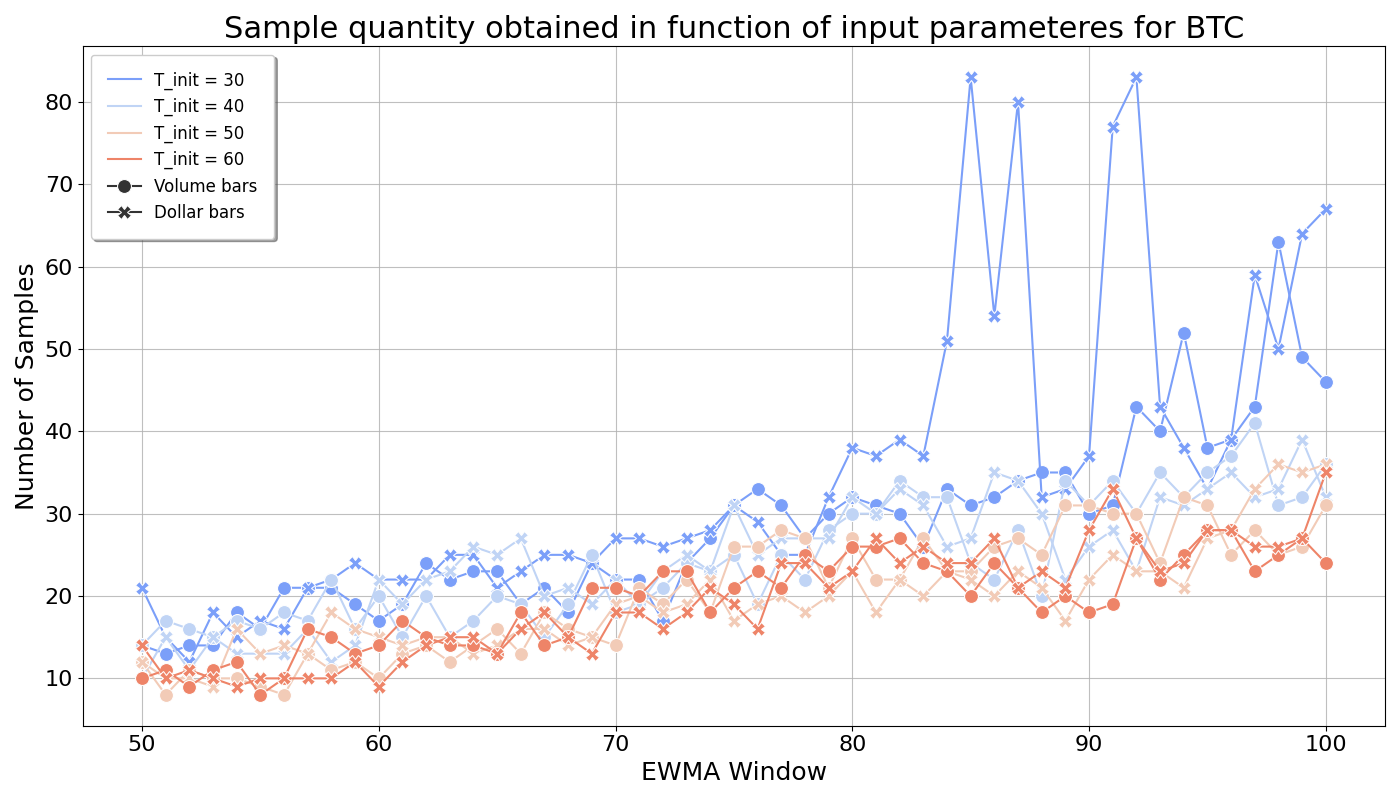
\includegraphics[width=0.9\textwidth]{./figures/barrido_parametros_imbalance_btc.png}
    \caption{Número de barras obtenido en datos de BTC}
    \label{fig:barrido-btc}
\end{figure}

\begin{figure}[H]
    \centering
    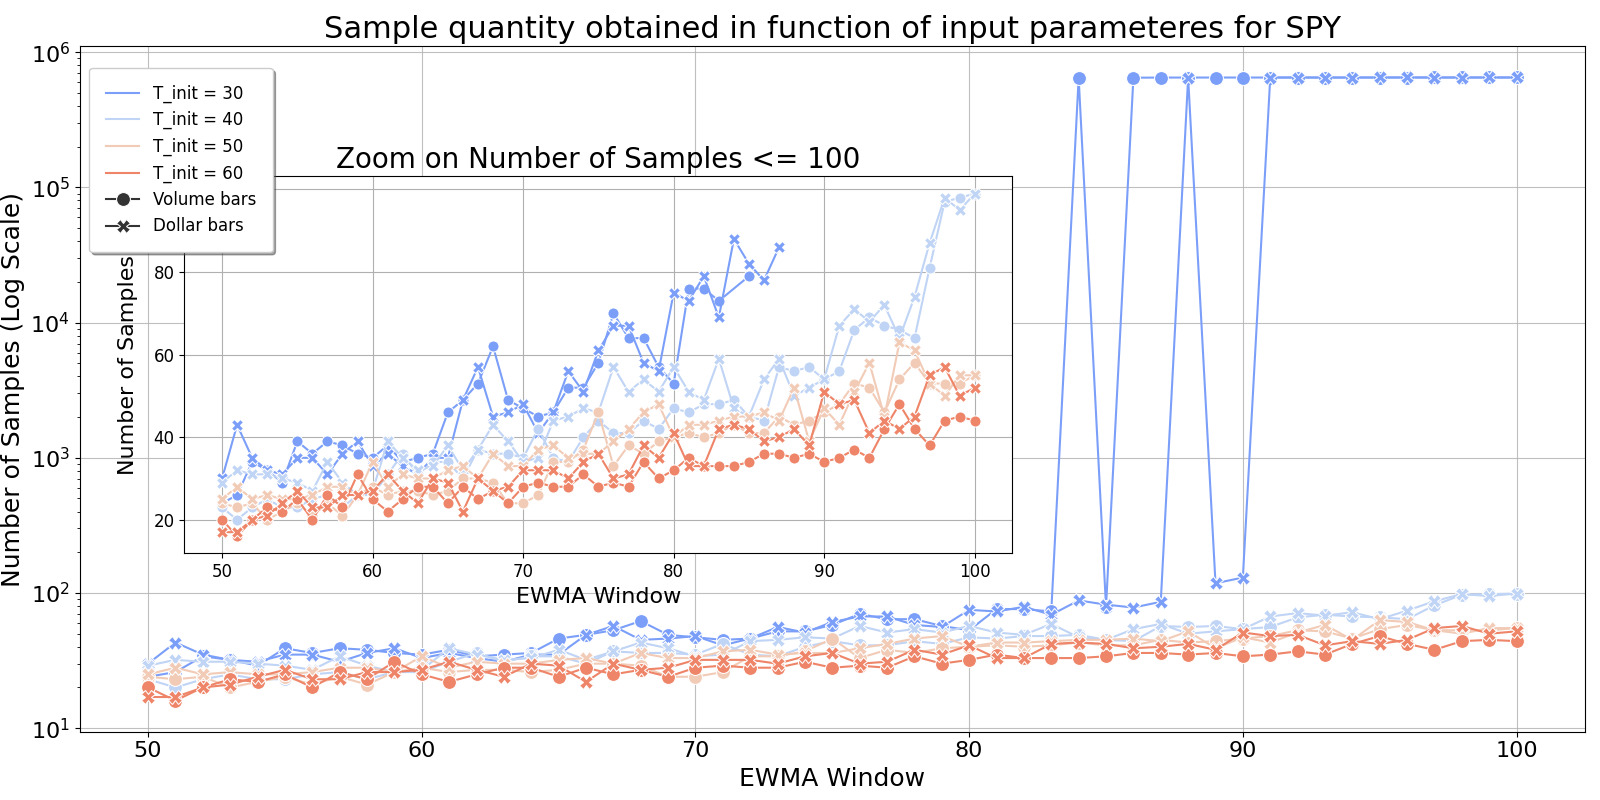
\includegraphics[width=0.9\textwidth]{./figures/barrido_parametros_imbalance_spy.png}
    \caption{Número de barras obtenido en datos del SPY}
    \label{fig:barrido-spy}
\end{figure}

Este comportamiento muestra un problema crítico en la implementación: la dinámica de generación de barras tiende a explotar, 
tal y como se muestra en la figura \ref{fig:explo-spy}. A medida que se van generando nuevas barras, el umbral de desequilibrio,
es decir, el producto de la multiplicacion del tamaño esperado de la barra por el desequilibrio esperado, provoca que el umbral de
desequilibrio sea cada vez mayor.

\begin{figure}[H]
    \centering
    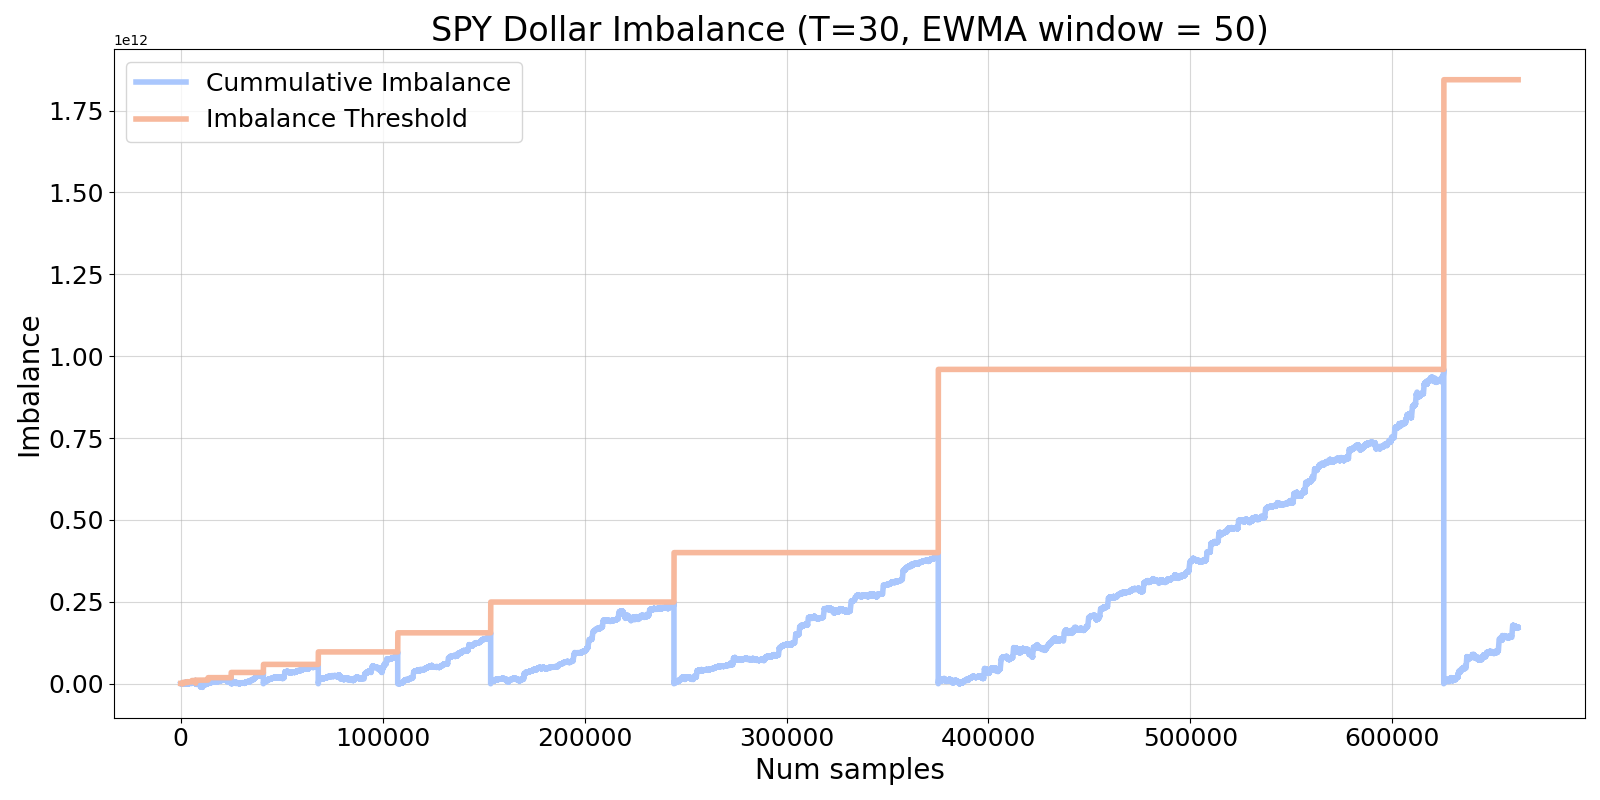
\includegraphics[width=0.9\textwidth]{./figures/spy_volume_explo.png}
    \caption{Explosión del umbral de desequilibrio en SPY}
    \label{fig:explo-spy}
\end{figure}

Para hacer frente a este problema, algunos investigadores han propuesto modificaciones 
a la implementación sugerida, tales como establecer un límite máximo al número esperado 
de ticks por barra o seleccionar directamente un umbral fijo de desequilibrio \cite{quant_finance_stack_exchange}. 

\subsection{Resultados} \label{sec:resultado-imbalance}
Para este trabajo, se ha optado por aplicar la metodología con umbrales de desequilibrio fijos, definidos experimentalmente.
Para cada activo y tipo de desequilibrio se ha seleccionado un umbral distinto, tal y como se muestra en la tabla \ref{tab:umbrales}.

\begin{table}[H]
    \centering
    \caption{Umbrales utilizados y numero de muestras obtenido}
    \begin{tabularx}{\textwidth}{|>{\centering\arraybackslash}X|>{\centering\arraybackslash}X|>{\centering\arraybackslash}X|>{\centering\arraybackslash}X|>{\centering\arraybackslash}X|>{\centering\arraybackslash}X|}
        \hline
        \textbf{Activo} & \textbf{Des- equilibrio} & \textbf{Umbral} & \textbf{Muestras iniciales} & \textbf{Muestras finales} & \textbf{Reducción (\%)} \\ \hline
        SPY & Volumen & $6 \times 10^{5}$ & 662,353 & 55,430 & 91.63\% \\ \hline
        SPY & Dólar & $1.5 \times 10^{8}$ & 662,353 & 85,228 & 87.13\% \\ \hline
        BTC & Volumen & $5 \times 10^{6}$ & 3,417,119 & 110,772 & 96.76\% \\ \hline
        BTC & Dólar & $1.5 \times 10^{10}$ & 3,417,119 & 1,003,756 & 70.63\% \\ \hline
    \end{tabularx}
    \label{tab:umbrales}
\end{table}

Los umbrales de desequilibrio se han definido con el fin de obtener una disminución significativa del numero de muestras de cada activo. Las 
disminuciones en la cantidad de datos van desde el 70\% para el desequilibrio de dolares de bitcoin, hasta el 96\% para el desequilibrio en volumen del
mismo activo.

En la Figura \ref{fig:btc-vol-imb-comp} se muestra una comparativa de los datos de precio originales de bitcoin y 
los de desequilibrio de volumen durante durante un segmento perteneciente al período de alta volatilidad ocasionada 
por la pandemia de COVID-19. Se puede observar cómo, para el mismo período de tiempo, las barras generadas mediante la metodología de desequilibrio 
son menos numerosas que las barras de minuto originales. 

Este fenómeno se debe a la agregación dinámica de los datos basada en la llegada de nueva información relevante, lo que permite una representación más frecuente
durante periodos de alta actividad de mercado.

\begin{figure}[H]
    \centering
    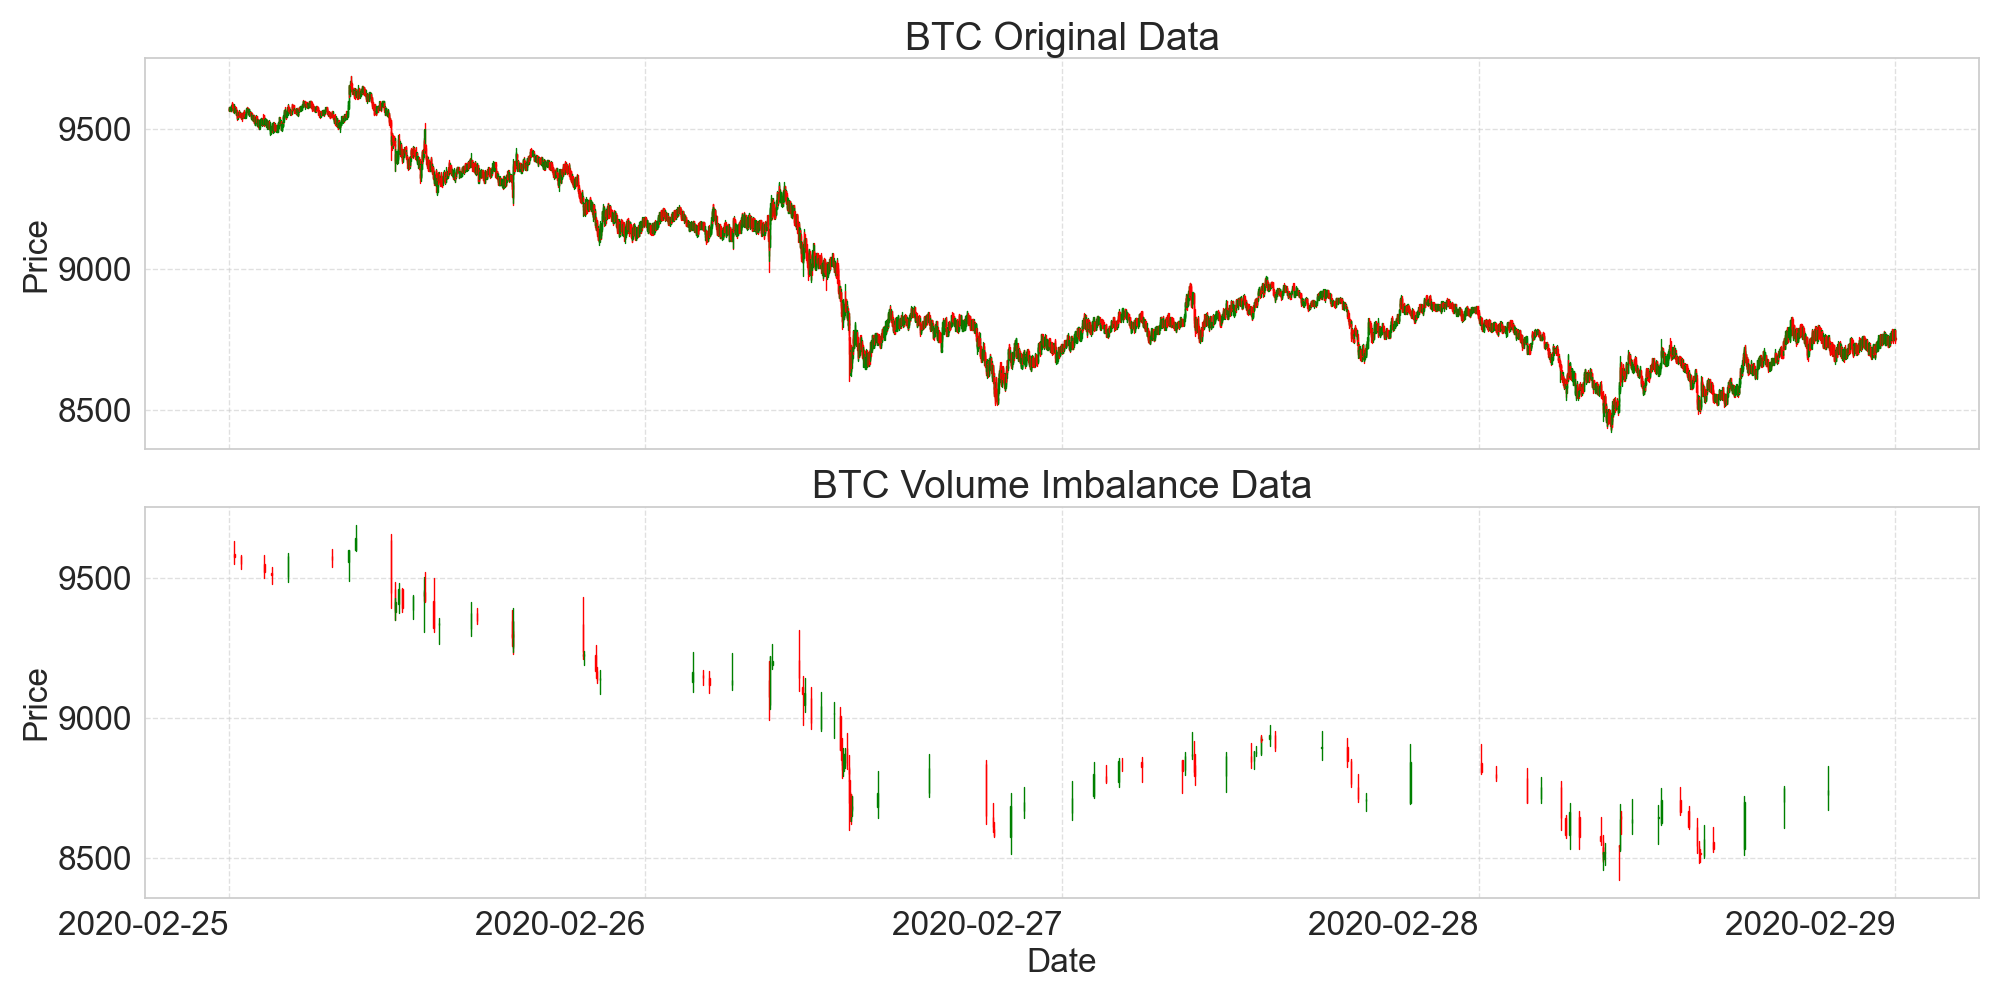
\includegraphics[width=0.9\textwidth]{./figures/btc_original_volume_imabalance_comp.png}
    \caption{Datos BTC originales y de Desequilibrio de Volumen}
    \label{fig:btc-vol-imb-comp}
\end{figure}

El artículo \cite{easley2012volume} expone que el uso de un marco temporal basado en volumen, en lugar de un 
marco cronológico tradicional, ofrece ventajas estadísticas significativas. Entre ellas, se destaca que 
este enfoque permite una reducción de los efectos estacionales intra-sesión y contribuye a una recuperación 
parcial de la normalidad en la distribución de los retornos financieros. Para evaluar esta afirmación, se 
ha aplicado la metodología de desequilibrio propuesta por los autores a los activos SPY y BTC, generando 
series temporales basadas en volumen y dinero.

Con el fin de verificar la normalidad de los retornos obtenidos mediante esta metodología, se han realizado 
pruebas estadísticas de normalidad, incluyendo los tests de Kolmogorov-Smirnov, Anderson-Darling y Jarque-Bera, 
cuyos resultados se resumen en la Tabla \ref{tab:normality_results}. Los resultados muestran que las series 
temporales originales de ambos activos presentan una desviación significativa de la normalidad, con valores 
extremadamente elevados de curtosis y asimetría, especialmente en el caso del SPY. 

Tras la aplicación de barras dinámicas basadas en volumen y dolares, se observa una reducción considerable 
en la curtosis y asimetría de los retornos. En particular, las barras basadas en volumen han demostrado 
ser más efectivas para aproximar la distribución de retornos a una forma más cercana a la normalidad. 
Estos resultados confirman en gran medida las hipótesis expuestas en \cite{easley2012volume}, 
evidenciando que el uso de un marco temporal basado en volumen contribuye a mejorar las propiedades 
estadísticas de las series temporales, aunque persisten algunas desviaciones de la normalidad, 
especialmente en los datos de BTC.


\begin{table}[H]
    \centering
    \caption{Resultados de pruebas estadísticas de normalidad para SPY y BTC}
    \begin{tabularx}{\textwidth}{|m{1cm}|m{1.35cm}|>{\centering\arraybackslash}X|>{\centering\arraybackslash}X|>{\centering\arraybackslash}X|>{\centering\arraybackslash}X|>{\centering\arraybackslash}X|>{\centering\arraybackslash}X|}
        \hline
        \textbf{Asset} & 
        \textbf{Series} & 
        \textbf{K-S Test \newline p-value} & 
        \textbf{Anderson-Darling \newline Statistic} & 
        \textbf{Jarque-Bera \newline p-value} & 
        \textbf{Skewness} & \textbf{Kurtosis} \\ \hline
        SPY & Original & 0.0 & 46037.02 & 0.0 & -11.83 & 2981.95 \\ \hline
        SPY & Volume & 0.0 & 1553.58 & 0.0 & -3.46 & 249.67 \\ \hline
        SPY & Dollar & 0.0 & 2947.14 & 0.0 & -4.24 & 383.73 \\ \hline
        BTC & Original & 0.0 & 646407.27 & 0.0 & 0.012 & 44.68 \\ \hline
        BTC & Volume & 0.0 & 3131.35 & 0.0 & -0.026 & 26.13 \\ \hline
        BTC & Dollar & 0.0 & 97255.28 & 0.0 & 0.070& 139.58 \\ \hline
    \end{tabularx}
    \label{tab:normality_results}
\end{table}

Además de las pruebas estadísticas, se han generado cuatro representaciones visuales que comparan 
las distribuciones de retornos de los activos SPY y BTC antes y después de aplicar la metodología 
basada en volumen y dinero. La Figura \ref{fig:histogram_comparison} muestra una comparativa de 
los histogramas de los retornos para el SPY y el BTC, donde se observa cómo la transformación 
mediante barras dinámicas logra atenuar la asimetría y la curtosis extrema presentes en las series 
temporales originales. 

Por otro lado, en la Figura \ref{fig:qqplot_comparison}, se presentan los QQ-plots correspondientes, 
que permiten evaluar visualmente el grado de ajuste de los retornos a una distribución normal. 
Los QQ-plots evidencian una mejora en la alineación con la diagonal en las series ajustadas, 
especialmente para el SPY, lo que sugiere una aproximación más cercana a la normalidad tras la 
aplicación de la metodología propuesta. 

\begin{figure}[H]
    \centering
    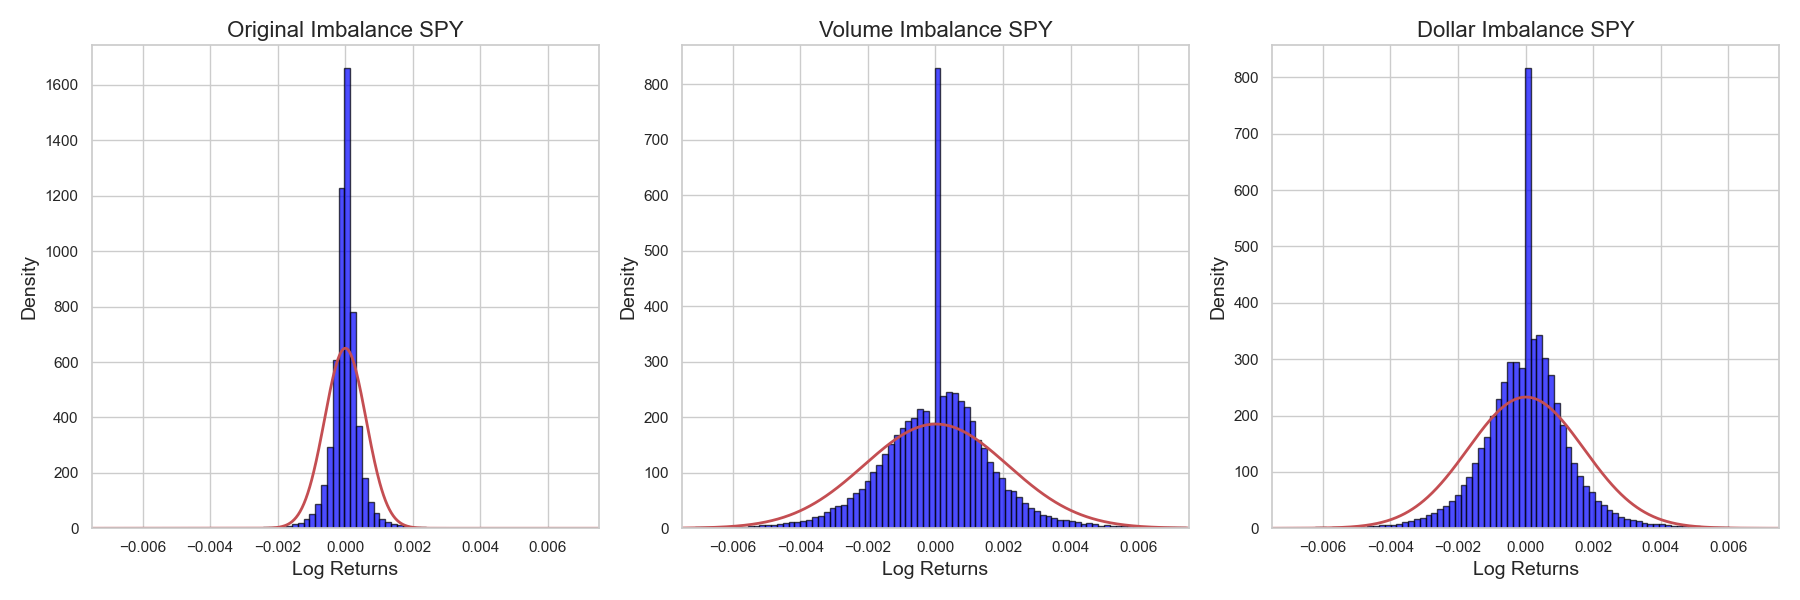
\includegraphics[width=0.8\textwidth]{figures/SPY_histogram_comparation.png}
    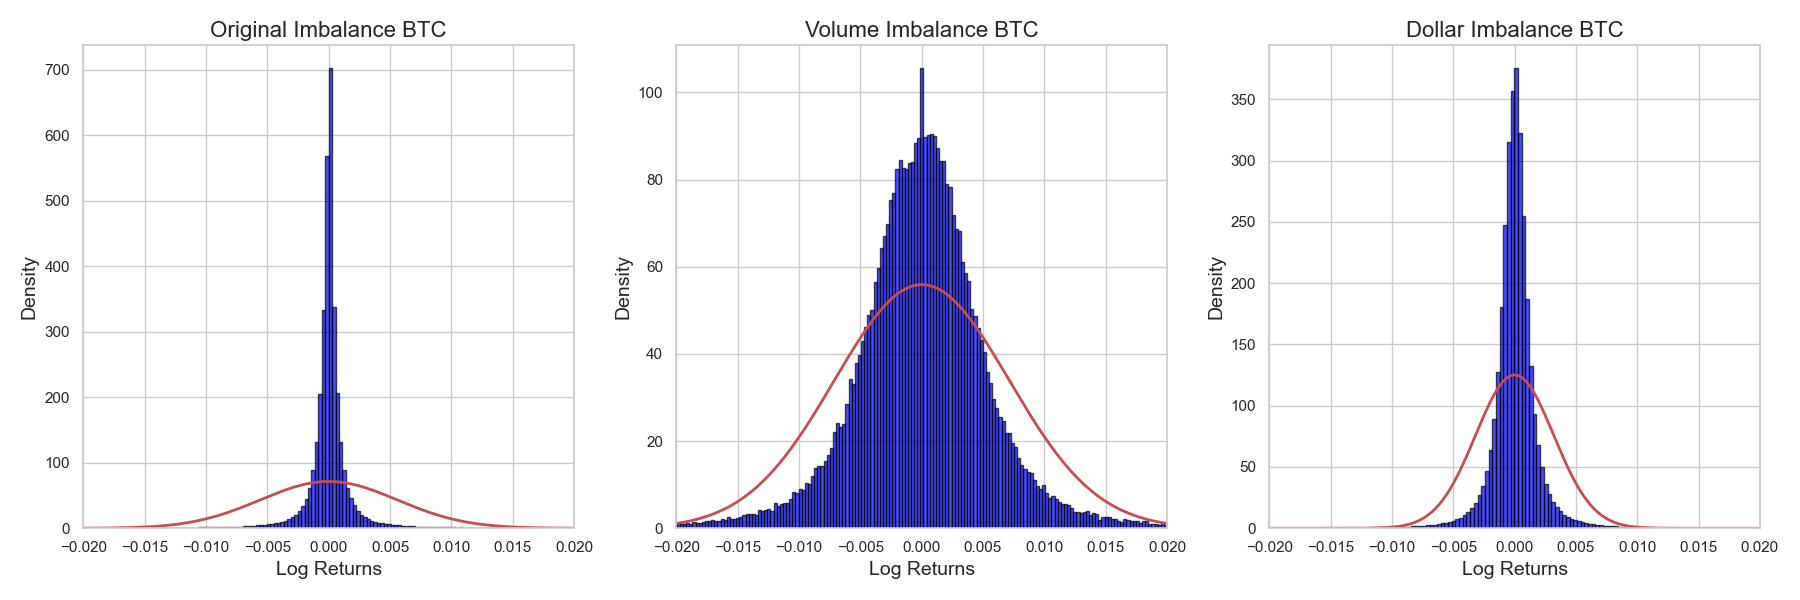
\includegraphics[width=0.8\textwidth]{figures/BTC_histogram_comparation.png}
    \caption{Comparativa de histogramas de los retornos del SPY (arriba) y BTC (abajo)}
    \label{fig:histogram_comparison}
\end{figure}

\begin{figure}[H]
    \centering
    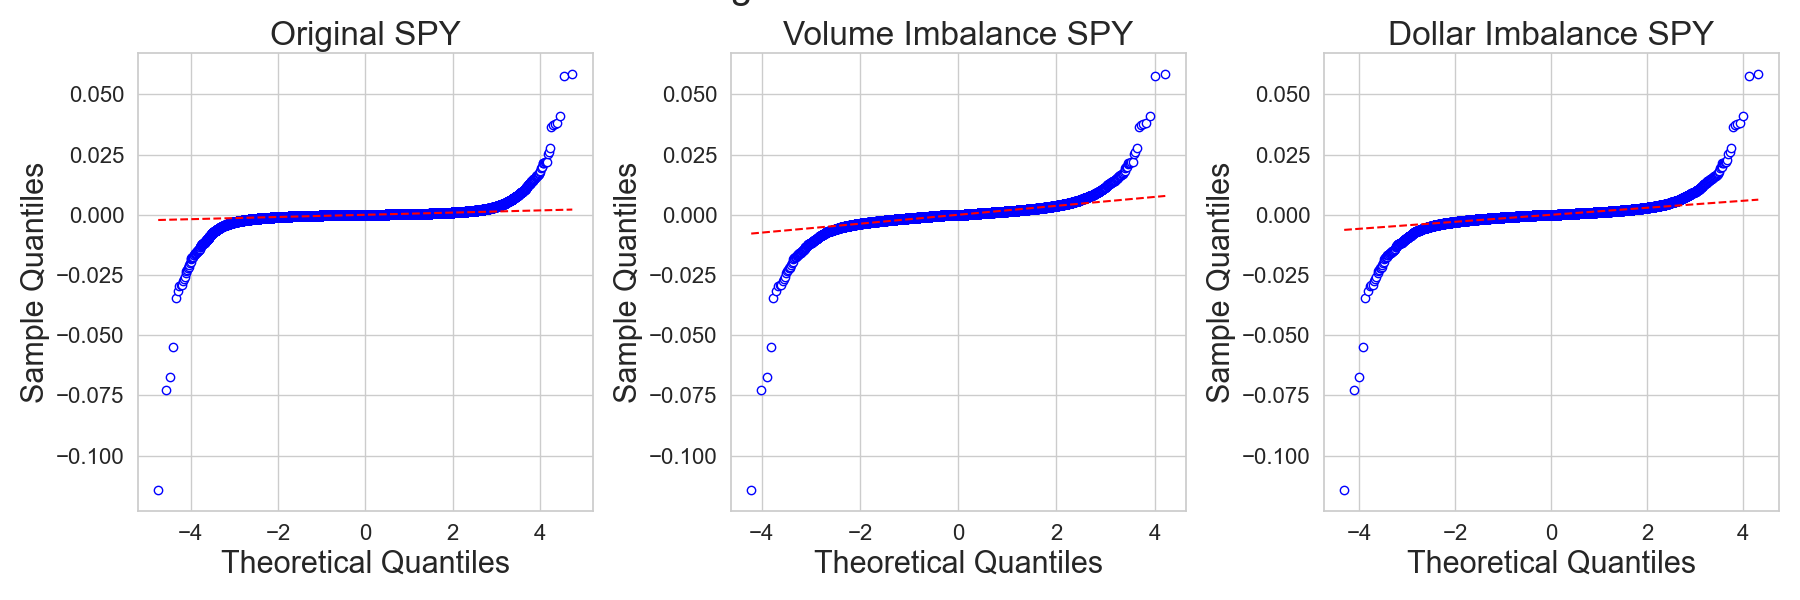
\includegraphics[width=0.8\textwidth]{figures/SPY_qq_comparison.png}
    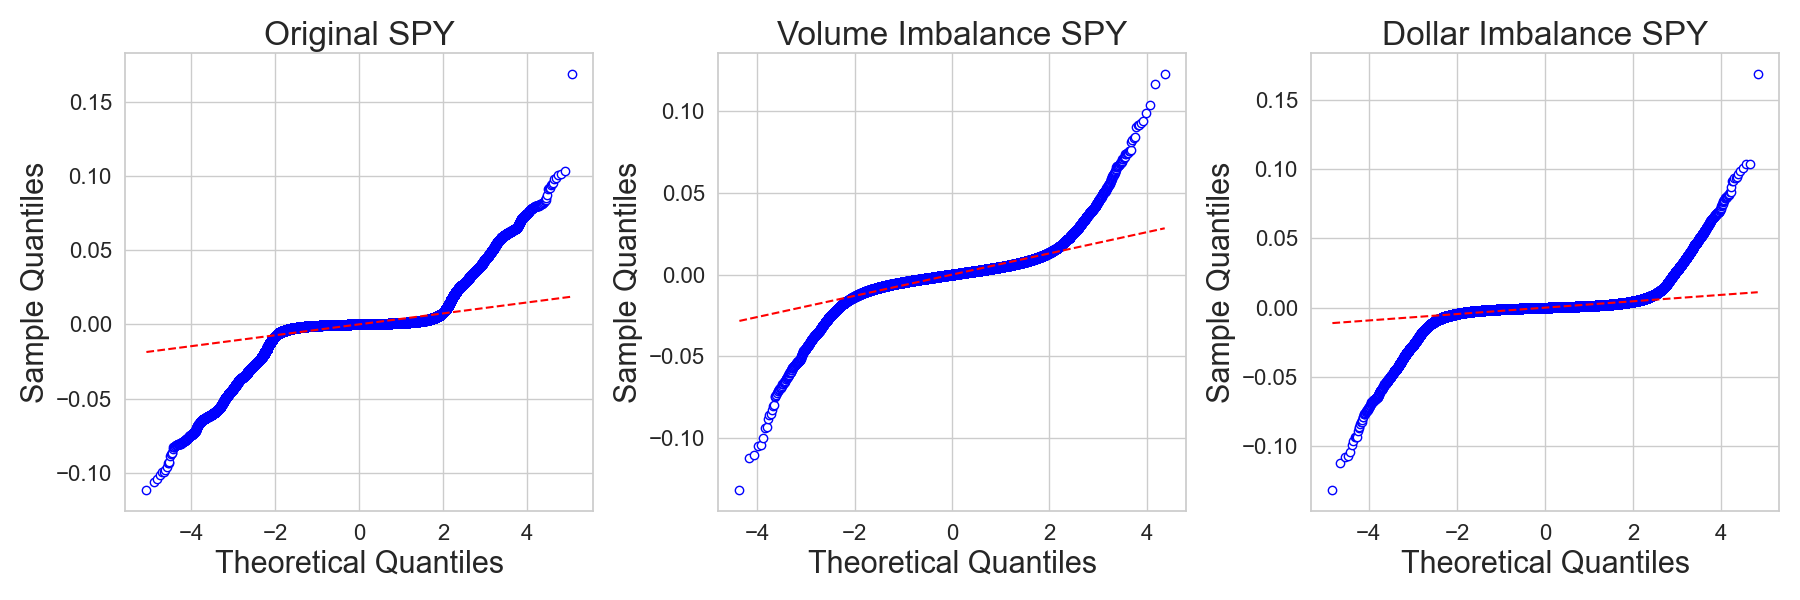
\includegraphics[width=0.8\textwidth]{figures/BTC_qq_comparison.png}
    \caption{Comparativa de QQ-plots de los retornos del SPY (arriba) y BTC (abajo)}
    \label{fig:qqplot_comparison}
\end{figure}

\chapter{Deep Reinforcement Learning}

\section{Introducción al Aprendizaje por Refuerzo (Reinforcement Learning)}

\subsection{Definición y Contexto General}

El \textit{Aprendizaje por Refuerzo} (Reinforcement Learning, RL) es una rama de la inteligencia 
artificial que se centra en cómo un agente aprende a tomar decisiones secuenciales optimizadas 
mediante la interacción con un entorno dinámico. A diferencia de otros tipos de aprendizaje, como 
el \textit{aprendizaje supervisado}, donde el modelo aprende patrones extraídos a partir de ejemplos 
previamente etiquetados, o el \textit{aprendizaje no supervisado}, donde el modelo busca patrones 
en datos sin etiquetas, el RL implica un aprendizaje activo donde el agente recibe retroalimentación 
en forma de recompensas o penalizaciones por las acciones que toma. Este proceso permite al 
agente aprender sin ejemplos de comportamiento óptimo, optimizando en su lugar una señal de recompensa.

\begin{figure}[H]
    \centering
    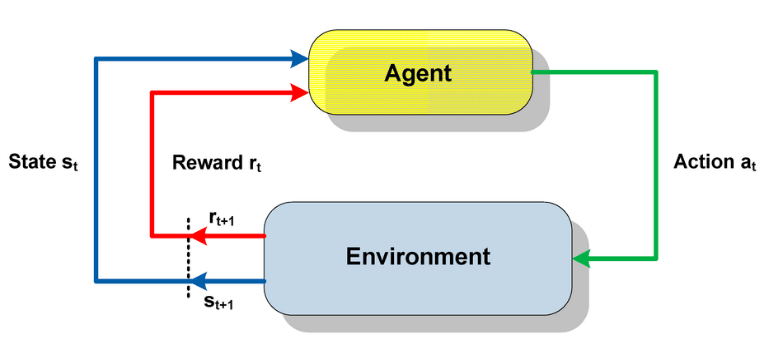
\includegraphics[width=0.5\textwidth]{./figures/A-brief-schema-of-Reinforcement-Learning-26.png}
    \caption{Esquema Reinforcement Learning}
    \label{fig:RF-schema}
\end{figure}

En cada paso de tiempo \(t\), el agente recibe una una observación \(O_t\) y una recompensa \(R_t\).
La observación recibida le permite ejecutar una acción \(A_t\), la cual provocará que el entorno cambie
y emita una nueva observación \(O_{t+1}\) y una nueva recompensa \(R_{t+1}\).

\subsubsection{Hipótesis de la Recompensa}

Una recompensa \(R_t\) es una señal de retroalimentación escalar que indica cómo de buena ha sido la accion 
tomada por el agente en el paso \(t-1\). 

A partir de esta señal de recopensa se formula
la \textit{hipótesis de la recompensa}, que afirma que en un esquema de aprendizaje por refuerzo, cualquier 
objetivo puede ser formalizado como el resultado de maximizar una recompensa acumulativa. Es decir, el objetivo del agente puede ser expresado como la maximización de una función de recompensa a lo 
largo del tiempo.

Esta función de recompensa se conoce como \textit{retorno} (\(G_t\)), y se define matemáticamente como el sumatorio
de las recompensas futuras, descontadas por un factor de descuento  \(\gamma\):

\begin{equation}
G_t = R_{t+1} + \gamma R_{t+2} + \gamma^2 R_{t+3} + \dots = \sum_{k=0}^{\infty} \gamma^k R_{t+k+1},
\end{equation}
El retorno \(G_t\) es lo que el agente intenta maximizar, y es la base sobre la cual se definen otros elementos como la función de valor.


Esto proporciona un marco ampliamente aplicable en situaciones donde 
las decisiones se toman en una serie de pasos, lo que incluye problemas de control robótico, juegos, 
y \textit{trading} financiero.

En el contexto particular del trading financiero, debido a la naturaleza secuencial y dinámica de 
los mercados, los agentes deben tomar decisiones basadas en información incompleta y en constante 
cambio, buscando maximizar una recompensa a largo plazo, como la rentabilidad de una cartera.


\subsection{Componentes Básicos del Aprendizaje por Refuerzo}

El aprendizaje por refuerzo se formaliza mediante un \textit{Proceso de Decisión de Markov} (MDP), 
que se define por un cuarteto \(\langle S, A, P, R \rangle\) el cual describe el problema de decisión.

Un MDP se representa por un conjunto de estados \(S\), 
un conjunto de acciones \(A\), una función de transición de estados \(P(s'|s, a)\), y una función de 
recompensa \(R(s, a)\). El objetivo del agente es aprender una política \(\pi(a|s)\) que maximice la 
recompensa acumulada a lo largo del tiempo.

Un proceso de decisión se dice que es Markov si la probabilidad de transición depende únicamente
del estado y acción actuales, no de la historia completa:

\begin{equation}
p(r, s' | S_t, A_t) = p(r, s' | H_t, A_t),
\end{equation}

donde $H_t$ es la \textit{Historia} en el instante $t$.

Esto significa que el estado contiene toda la información relevante de la historia, siendo la historia 
la secuencia completa de observaciones, acciones y recompensas. No quiere decir que la historia contenga
toda la información, sino más bien que el añadir cualquier información adicional no afectará la decisión.

\begin{itemize}
    \item \textbf{Estados (\(S\))}: Representan todas las posibles situaciones en las que se puede 
    encontrar el agente dentro del entorno.
    \item \textbf{Acciones (\(A\))}: Conjunto de todas las decisiones que el agente puede tomar 
    desde cualquier estado dado.
    \item \textbf{Función de Transición de Estados (\(P\))}: Describe la probabilidad de transitar 
    del estado \(s\) al estado \(s'\) como resultado de realizar una acción \(a\), es decir, \(P(s'|s, a)\).
    \item \textbf{Función de Recompensa (\(R\))}: Proporciona una recompensa que el agente 
    recibe al transitar del estado \(s\) al estado \(s'\) al realizar la acción \(a\), es decir, \(R(s, a, s')\).
\end{itemize}

El objetivo del agente en RL es aprender una \textit{política} \(\pi(a|s)\) que maximice la recompensa 
acumulada a lo largo del tiempo. La política puede ser determinista, donde una acción específica es 
seleccionada para cada estado, o estocástica, donde se asigna una distribución de probabilidad a las
acciones en cada estado.

Un concepto fundamental en RL es la \textit{función de valor}, que mide cuán favorable es un estado 
o una acción en términos de la recompensa esperada:

\begin{itemize}
    \item \textbf{Función de Valor de Estado (\(V^{\pi}(s)\))}: Estima la recompensa total esperada 
    comenzando desde el estado \(s\) y siguiendo la política \(\pi\). Formalmente, se define como:
    \begin{equation}
    V^{\pi}(s) = \mathbb{E}\left[\sum_{t=0}^{\infty} \gamma^t R(s_t, a_t) \mid s_0 = s, \pi\right],
    \end{equation}
    donde \(\gamma \in (0, 1)\) es el factor de descuento que determina la importancia de las 
    recompensas futuras. Esta función refleja el valor a largo plazo de estar en un estado particular 
    bajo una política dada.

    La función de valor del estado, \(V^{\pi}(s)\), trata de cuantificar \textit{cómo de bueno} es 
    estar en un estado \(s\) cuando se sigue una política \(\pi\).

    \item \textbf{Función de Valor de Acción (\(Q^{\pi}(s, a)\))}: Extiende la función de valor del 
    estado para considerar no solo el estado \(s\), sino también la acción \(a\) tomada en ese estado. 
    Esta función estima la recompensa total esperada al tomar la acción \(a\) en el estado \(s\) y 
    seguir la política \(\pi\) posteriormente:
    \begin{equation}
    Q^{\pi}(s, a) = \mathbb{E}\left[\sum_{t=0}^{\infty} \gamma^t R(s_t, a_t) \mid s_0 = s, a_0 = a, \pi\right]
    \end{equation}
    La función de valor de la acción, \(Q^{\pi}(s, a)\), trata de medir \textit{cómo de buena} es una 
    acción \(a\) específica en un estado \(s\) determinado cuando se sigue la política \(\pi\) después.
 
\end{itemize}

En resumen, la función del valor del estado, \(V^{\pi}(s)\), mide cuán bueno es estar en un estado dado 
bajo una política \(\pi\), mientras que \(Q^{\pi}(s, a)\) mide cuán buena es una acción específica en 
ese estado.

\subsubsection{Política}

La \textbf{política} (\textit{policy}) es la función que guía la selección de acciones en función del estado actual del entorno. Existen dos variantes principales:

\begin{itemize}
    \item \textbf{Política determinista:} Representada como $\pi(s)$, esta política asigna una acción específica $a$ a cada estado $s$. Formalmente, $\pi(s) = a$, donde $a$ es la acción elegida para el estado $s$.

    \item \textbf{Política estocástica:} Denotada como $\pi(a|s)$, esta política define una distribución de probabilidad sobre las acciones posibles. Es decir, $\pi(a|s) = \mathbb{P}(A = a \mid S = s)$, donde $a$ es seleccionada según la probabilidad correspondiente en el estado $s$.
\end{itemize}

La política determinista es útil en entornos estables, mientras que la estocástica es preferible en situaciones con alta incertidumbre o donde la exploración es necesaria.


\subsubsection{Exploración vs. Explotación}

En el Aprendizaje por Refuerzo, un desafío clave es el equilibrio entre \textit{exploración} y 
\textit{explotación}. Este balance es fundamental para el aprendizaje efectivo del agente:

\begin{itemize}
    \item \textbf{Exploración}: El agente intenta nuevas acciones para descubrir si existen mejores 
    recompensas disponibles. La exploración es crucial cuando el agente no tiene suficiente conocimiento 
    del entorno y necesita recolectar más información.
    \item \textbf{Explotación}: El agente selecciona la mejor acción conocida basada en su 
    política actual para maximizar la recompensa inmediata. La explotación se basa en la información 
    acumulada y tiene como objetivo maximizar la recompensa a corto plazo.
\end{itemize}

El \textit{trade-off} entre exploración y explotación es crucial porque un agente que explora 
demasiado podría no aprovechar las recompensas conocidas, mientras que un agente que explota 
demasiado podría perder oportunidades para descubrir estrategias más efectivas. 

Existen diversas estrategias para manejar este trade-off, como la \textit{política epsilon-greedy}, 
donde con una probabilidad \(\epsilon\), el agente explora una acción al azar, y con 
una probabilidad \(1-\epsilon\), explota la mejor acción conocida. El valor de \(\epsilon\) 
generalmente disminuye a medida que el agente gana más confianza en su política, lo que permite 
una mayor explotación con el tiempo.


\subsection{El Problema de la Toma de Decisiones Óptimas en el Tiempo - La ecuación de Bellman}


En el contexto del aprendizaje por refuerzo, uno de los problemas fundamentales es 
\textbf{cómo un agente puede tomar decisiones óptimas en situaciones donde las consecuencias de 
sus acciones no son inmediatas, sino que se extienden en el tiempo}. Las decisiones actuales no 
solo influyen en la recompensa inmediata, sino también en las recompensas futuras. 

Algunas decisiones pueden ofrecer beneficios inmediatos pero desviar al agente de un objetivo 
más valioso en el futuro, mientras que otras pueden tener un alto coste presente, pero ser 
cruciales para un éxito posterior.

Este desafío, conocido como el problema de la maximización del retorno total esperado, 
requiere una estrategia que considere tanto las recompensas inmediatas como las futuras, 
ponderadas para reflejar su importancia relativa. La ecuación de Bellman se introduce como 
una herramienta esencial para descomponer este problema global en subproblemas más manejables, 
\textbf{permitiendo al agente evaluar el impacto a largo plazo de sus decisiones actuales de 
manera eficiente y sistemática}.

La ecuación de Bellman descompone el problema global de maximización del retorno total 
esperado en subproblemas más manejables. 

El valor de un estado \(V^\pi(s)\) bajo una política \(\pi\) se define como el valor esperado 
del retorno total que se puede obtener comenzando desde ese estado \(s\) y siguiendo la política 
\(\pi\). Matemáticamente, se expresa como:

\begin{equation}
V^\pi(s) = \mathbb{E}_\pi \left[ \sum_{k=0}^{\infty} \gamma^k R_{t+k+1} \mid s_t = s \right],
\end{equation}

Esta ecuación describe el valor esperado del retorno acumulado desde el estado \(s\). 
Para hacerla más práctica, es posible descomponer esta expresión en dos partes: la 
recompensa inmediata y el valor de los estados futuros. Separando el primer término de 
la suma, se obtiene:

\begin{equation}
V^\pi(s) = \mathbb{E}_\pi \left[ R_{t+1} + \gamma \sum_{k=1}^{\infty} \gamma^{k-1} R_{t+k+1} \mid s_t = s \right],
\end{equation}

Aquí, \(R_{t+1}\) es la recompensa inmediata obtenida al tomar una acción en el estado \(s\), 
y el resto de la suma representa el valor descontado de las recompensas futuras, que 
corresponde al valor de \(V^\pi(s_{t+1})\). De esta forma, es posible reescribir la ecuación como:

\begin{equation}
V^\pi(s) = \mathbb{E}_\pi \left[ R_{t+1} + \gamma V^\pi(s_{t+1}) \mid s_t = s \right],
\end{equation}

Para expandir esta expectativa, se consideran todas las posibles acciones \(a\) que el agente 
puede tomar en el estado \(s\), y todas las posibles transiciones a estados futuros \(s'\) 
después de tomar la acción \(a\). Esto lleva a la forma completa de la ecuación de Bellman:

\begin{equation}
V^\pi(s) = \sum_{a} \pi(a|s) \sum_{s'} P(s'|s,a) \left[ R(s,a,s') + \gamma V^\pi(s') \right],
\end{equation}

Aquí:
\begin{itemize}
    \item \(\pi(a|s)\) es la probabilidad de tomar la acción \(a\) dado el estado \(s\).
    \item \(P(s'|s,a)\) es la probabilidad de transición al estado \(s'\) dado el estado \(s\) y la acción \(a\).
    \item \(R(s,a,s')\) es la recompensa inmediata por la transición de \(s\) a \(s'\) mediante la acción \(a\).
    \item \(\gamma\) es el factor de descuento, que pondera la importancia relativa de las recompensas futuras.
\end{itemize}

Esta ecuación establece que el valor de un estado es la suma de la recompensa inmediata 
y el valor futuro esperado, ponderado por las probabilidades de las acciones y las 
transiciones de estado. Así, la ecuación de Bellman permite calcular los valores de 
los estados de manera recursiva, evaluando tanto el impacto inmediato como el impacto a 
largo plazo de las decisiones actuales.

\subsubsection{Cálculo Numérico: Iteración de Valores}

Para calcular los valores \(V^\pi(s)\) numéricamente, se suele utilizar un método iterativo. 
Inicialmente, se asigna un valor arbitrario a cada estado, por ejemplo, \(V_0(s) = 0\) para 
todos los \(s\). Luego, estos valores se actualizan iterativamente utilizando la ecuación de 
Bellman:

\begin{equation}
V_{k+1}(s) = \max_{a} \sum_{s'} P(s'|s,a) \left[ R(s,a,s') + \gamma V_k(s') \right],
\end{equation}

El proceso comienza con los estados finales, cuyos valores se pueden calcular directamente. 
Para un estado final \(s_f\), donde no hay más decisiones ni transiciones posibles, el 
valor \(V^\pi(s_f)\) se define como:

\begin{equation}
V^\pi(s_f) = 0 \quad \text{(sin recompensas futuras)},
\end{equation}

o, si hay una recompensa final al alcanzar \(s_f\):

\begin{equation}
V^\pi(s_f) = R_f,
\end{equation}

Este proceso se repite hasta que los valores convergen, es decir, cuando \(V_{k+1}(s) 
\approx V_k(s)\) para todos los estados \(s\).


\subsection{Métodos Clásicos de Aprendizaje por Refuerzo}

Existen varios algoritmos clásicos de RL que permiten a los agentes aprender políticas óptimas. Los 
algoritmos se clasifican principalmente en dos categorías: \textit{on-policy} y \textit{off-policy}. 
Estos términos se refieren a la relación entre la política que se está evaluando y mejorando y la 
política que se está utilizando para generar las acciones y, por lo tanto, las experiencias (es decir, 
las transiciones estado-acción-recompensa) que se utilizan para actualizar el modelo.

Un algorítmo de tipo \textit{on-policy} es aquel en el que la política que se optimiza es la misma que 
se utiliza para interactuar con el entorno y generar experiencias. Es decir, se evalúa y mejora la misma
política que se sigue durante el proceso de aprendizaje. Mientras que un algorítmo del tipo \textit{off-policy}
es aquel en el que la política que se intenta optimizar es diferente de la política utilizada para generar
las experiencias. Esto permite optimizar una política mientras se sigue otra.

Un ejemplo de algoritmos representativos de cada una de estas categorías son los siguientes:

\begin{itemize}
    \item \textbf{Q-learning}: Un algoritmo \textit{off-policy} que aprende la función de valor de 
    acción \(Q(s, a)\) actualizando iterativamente las estimaciones en función de las recompensas recibidas:
    \begin{equation}
    Q(s_t, a_t) \leftarrow Q(s_t, a_t) + \alpha \left[r_{t+1} + \gamma \max_{a'} Q(s_{t+1}, a') - Q(s_t, a_t)\right],
    \end{equation}
    donde \(\alpha\) es la tasa de aprendizaje. Como algoritmo \textit{off-policy}, Q-learning aprende la 
    política óptima independientemente de la política que el agente sigue durante la exploración. 
    Esto significa que la política utilizada para seleccionar acciones (\textit{behavior policy}) 
    puede ser diferente de la política que se está optimizando (\textit{target policy}).

    \item \textbf{SARSA}: Un algoritmo \textit{on-policy} que, a diferencia de Q-learning, sigue la 
    política actual para actualizar la función \(Q(s, a)\). La actualización en SARSA se realiza 
    utilizando la acción que el agente realmente toma, lo que significa que la política utilizada 
    para seleccionar acciones es la misma que se está optimizando:
    \begin{equation}
    Q(s_t, a_t) \leftarrow Q(s_t, a_t) + \alpha \left[r_{t+1} + \gamma Q(s_{t+1}, a_{t+1}) - Q(s_t, a_t)\right],
    \end{equation}
    Como resultado, SARSA tiende a ser más conservador en su aprendizaje, ya que la política sigue 
    siendo consistente entre el aprendizaje y la ejecución.

\end{itemize}


Los algoritmos \textit{on-policy}, como SARSA, tienen la ventaja de ser coherentes con la política 
actual, lo que puede resultar en un aprendizaje más seguro y estable en entornos dinámicos. Sin embargo, 
pueden ser menos eficientes, ya que dependen exclusivamente de las experiencias generadas por la misma 
política que se está optimizando, lo que puede limitar la exploración. Por otro lado, los algoritmos 
off-policy, como Q-Learning, son más flexibles y permiten un aprendizaje más eficiente al poder optimizar 
una política óptima mientras se sigue una política diferente, más exploratoria. Sin embargo, esta 
flexibilidad puede conllevar complejidad adicional y posibles problemas de estabilidad durante el 
proceso de aprendizaje.

Estos métodos son fundamentales para entender cómo los agentes pueden aprender a tomar decisiones 
óptimas en entornos inciertos y son la base sobre la cual se construyen los métodos más avanzados 
como el \textit{Deep Reinforcement Learning} (DRL).


\section{Evolución del Deep Reinforcement Learning (DRL)}

\subsection{Combinación con Redes Neuronales}

El \textit{Deep Reinforcement Learning} (DRL) surge como una evolución natural del 
\textit{Aprendizaje por Refuerzo} (RL) tradicional, combinando sus principios con la potencia 
de las redes neuronales profundas (\textit{Deep Learning}). Mientras que los métodos clásicos 
de RL, como el \textit{Q-learning}, son eficaces en problemas con espacios de estados discretos 
y de baja dimensionalidad, presentan limitaciones significativas cuando se aplican a entornos 
complejos y continuos.

El uso de redes neuronales como aproximadores de funciones en RL permitió superar estas 
limitaciones. Las redes neuronales profundas son capaces de procesar entradas de alta 
dimensionalidad y de extraer características complejas directamente de los datos sin la necesidad 
de diseñar manualmente las características relevantes. 

\subsection{Principales Enfoques y Algoritmos de DRL}

El desarrollo de DRL ha dado lugar a diversos enfoques que combinan RL y Deep Learning, dando 
lugar a algoritmos innovadores que han transformado la forma en que se aborda el aprendizaje 
por refuerzo en entornos complejos. A continuación, se presentan los enfoques principales en 
DRL, junto con ejemplos representativos de cada uno.

\subsubsection{Métodos Basados en Funciones de Valor}

Los métodos basados en funciones de valor son aquellos en los que el objetivo es aprender 
una función que prediga el valor de tomar una acción en un estado dado. El ejemplo más 
destacado de este enfoque es el \textit{Deep Q-Network} (DQN). DQN, introducido por 
\textit{DeepMind} \cite{deepmind_drl}, utiliza redes neuronales profundas para aproximar la función \(Q(s, a)\), 
lo que permitió manejar entornos con espacios de estados grandes y continuos.

En DQN, una red neuronal recibe como entrada el estado del entorno y produce una estimación 
de los valores \(Q(s, a)\) para cada acción posible. La red se entrena utilizando el 
algoritmo de \textit{Q-learning} tradicional, pero con varias modificaciones clave para 
estabilizar el aprendizaje, como el uso de un \textit{buffer} de \textit{replay} para 
almacenar transiciones de experiencias pasadas y el uso de una red objetivo 
(\textit{target network}) que se actualiza periódicamente para reducir la inestabilidad 
en la actualización de los valores \(Q\).

\subsubsection{Métodos de Gradiente de Política}

Los métodos de gradiente de política representan un enfoque alternativo en DRL, en el cual, 
en lugar de aprender una función de valor, el agente aprende directamente una política 
parametrizada \(\pi_{\theta}(a|s)\) que maximiza la recompensa esperada. La principal 
ventaja de estos métodos es su capacidad para manejar espacios de acción continuos y 
para aprender políticas estocásticas.

Un algoritmo básico dentro de esta categoría es \textit{REINFORCE}, que utiliza el gradiente 
de la recompensa esperada para actualizar los parámetros de la política. Aunque REINFORCE es 
sencillo y conceptualmente atractivo, su principal limitación es la alta varianza en las 
estimaciones del gradiente, lo que puede llevar a un aprendizaje lento y poco estable.

\subsubsection{Métodos Actor-Critic}

Los métodos \textit{Actor-Critic} combinan lo mejor de ambos mundos al utilizar tanto una 
función de valor como una política parametrizada. En este enfoque, el \textit{actor} es 
responsable de seleccionar las acciones basadas en la política \(\pi_{\theta}(a|s)\), mientras 
que el \textit{crítico} estima el valor de la política actual utilizando una función de valor 
\(V^{\pi}(s)\) o \(Q^{\pi}(s, a)\).

Un ejemplo notable es el \textit{Asynchronous Advantage Actor-Critic} (A3C), que introduce 
el concepto de ventaja (\textit{advantage}), definida como la diferencia entre el valor de 
la acción y el valor esperado del estado (\(A(s, a) = Q(s, a) - V(s)\)). A3C mejora la 
estabilidad del aprendizaje al usar múltiples actores que interactúan con copias del entorno 
en paralelo, lo que también mejora la eficiencia computacional.

\section{Proximal Policy Optimization (PPO) y su Implementación}

\subsection{Introducción a Proximal Policy Optimization (PPO)}

Proximal Policy Optimization (PPO) es un algoritmo de \textit{Deep Reinforcement Learning} 
(DRL) desarrollado por \textit{OpenAI}, que ha demostrado ser exitoso en una amplia variedad 
de tareas, desde el control robótico hasta videojuegos complejos como \textit{Dota 2}. 
PPO es un método de gradiente de política (\textit{Policy Gradient}), lo que significa 
que aprende directamente de la experiencia en tiempo real generada por el agente en su 
interacción con el entorno, a diferencia de los métodos basados en \textit{Q-learning}, 
que pueden aprender de datos almacenados.

PPO fue diseñado para encontrar un equilibrio entre la eficiencia de la muestra, la facilidad 
de implementación y la estabilidad en el entrenamiento. Esto lo convierte en una herramienta 
potente y versátil para abordar problemas de aprendizaje por refuerzo en entornos continuos y 
de alta dimensionalidad.

En este trabajo, PPO se utilizará para la generación de estrategias de trading, aprovechando 
su capacidad para manejar entornos complejos y dinámicos como los mercados financieros. Este 
algoritmo ha sido seleccionado debido a su robustez y simplicidad en la implementación, 
características que lo hacen ideal para desarrollar una estrategia de trading que pueda 
adaptarse a las condiciones cambiantes del mercado.

PPO fue presentado por primera vez en el paper de \textit{Schulman et al.} titulado 
"\textit{Proximal Policy Optimization Algorithms}" \cite{Schulman2017}, que ha sido ampliamente 
citado en la literatura de aprendizaje por refuerzo debido a su enfoque innovador y eficaz.

Este algorítmo ha sido utilizado con éxito en la creación de estrategias de trading 
algorítmico debido a su capacidad de manejar la inestabilidad inherente a los entornos 
financieros en constante cambio. Estudios como el de Zhang et al. (2020) \cite{pricope2021review} han demostrado 
la robustez de este algoritmo en la optimización de portafolios y la adaptación a fluctuaciones repentinas en el mercado de acciones

\subsection{Descripción Técnica de PPO}

PPO introduce varias mejoras clave en la optimización de políticas para garantizar un 
aprendizaje más estable. A diferencia de otros métodos que pueden permitir grandes cambios 
en la política, PPO limita estos cambios para evitar desestabilizar el proceso de entrenamiento.

\subsubsection{Problemas en el Aprendizaje por Refuerzo}

A diferencia del aprendizaje supervisado, donde se trabaja con un conjunto de datos estático, 
en el aprendizaje por refuerzo el conjunto de datos cambia constantemente porque el agente 
genera sus propios datos a medida que interactúa con el entorno. Esto provoca que las 
distribuciones de las observaciones y las recompensas varíen durante el entrenamiento, 
lo que puede causar inestabilidad.

Además, el aprendizaje por refuerzo es altamente sensible a la configuración de hiperparámetros 
y la inicialización. Por ejemplo, una tasa de aprendizaje demasiado alta puede llevar a que 
las actualizaciones de la política desvíen al agente hacia regiones del espacio de parámetros 
donde su desempeño se deteriora drásticamente, sin posibilidad de recuperación.

\subsubsection{Función de Objetivo en PPO}

PPO aborda estos problemas proponiendo una función de objetivo que maximiza la recompensa 
esperada mientras limita las actualizaciones de la política para evitar cambios excesivos. 
La función de objetivo en PPO se expresa como:

\begin{equation}
L^{PPO}(\theta) = \mathbb{E}_t \left[ \min\left(r_t(\theta) \hat{A}_t, \text{clip}(r_t(\theta), 1 - \epsilon, 1 + \epsilon) \hat{A}_t \right) \right],
\end{equation}

Aquí, \( r_t(\theta) \) es la razón de probabilidad entre la nueva política \(\pi_\theta(a|s)\) 
y la política antigua \(\pi_{\theta_{\text{old}}}(a|s)\):

\begin{equation}
r_t(\theta) = \frac{\pi_\theta(a_t|s_t)}{\pi_{\theta_{\text{old}}}(a_t|s_t)}
\end{equation}

El término \(\hat{A}_t\) es la estimación de la ventaja, que mide cuánto mejor o peor fue la 
acción tomada en comparación con lo esperado. El operador \textit{clip} limita el valor de 
\(r_t(\theta)\) dentro del rango \([1 - \epsilon, 1 + \epsilon]\), con \(\epsilon\) típicamente 
igual a 0.2, para prevenir que las actualizaciones de la política sean demasiado agresivas,
manteniendo así la estabilidad del entrenamiento.

\subsubsection{Ventaja y Estimación del Valor}

Para calcular la ventaja \(\hat{A}_t\), PPO utiliza dos componentes:

\begin{itemize}
    \item \textbf{Retorno descontado}: Es la suma de las recompensas acumuladas, descontadas 
    por un factor \(\gamma\) que valora más las recompensas inmediatas.
    \item \textbf{Función de valor}: Estima el valor esperado de estar en un estado dado, 
    calculando la recompensa total esperada desde ese estado en adelante.
\end{itemize}

La ventaja se calcula restando la función de valor del retorno descontado, proporcionando 
una medida de si la acción tomada fue mejor o peor que el promedio esperado.

\subsubsection{Procedimiento de Entrenamiento}

PPO recolecta nuevas trayectorias de interacciones con el entorno en cada iteración, 
utilizando estas trayectorias para actualizar la política. A diferencia de otros métodos, 
no utiliza un \textit{replay buffer}, lo que significa que las experiencias se utilizan 
una sola vez para hacer la actualización, y luego se descartan.

Este proceso iterativo continúa hasta que las mejoras en la política se estabilizan, 
lo que indica que el algoritmo ha convergido. PPO equilibra la simplicidad y la robustez, 
permitiendo un entrenamiento estable incluso en entornos complejos y dinámicos.

\section{Implementación del Entorno de Entrenamiento con Gymnasium}

\subsection{Introducción a Gymnasium}

Gymnasium \cite{gymnasium2023} es una biblioteca de Python ampliamente utilizada en el campo del 
\textit{Reinforcement Learning} (RL) para crear, gestionar y probar entornos 
de simulación. Esta biblioteca es una evolución de OpenAI Gym, diseñada para 
facilitar la construcción de entornos personalizados y la evaluación de algoritmos 
de RL en una variedad de dominios, desde juegos sencillos hasta tareas más complejas 
como la robótica y el trading financiero.

La popularidad de Gymnasium se debe a su simplicidad y flexibilidad. Proporciona una 
interfaz estándar que permite a los desarrolladores de algoritmos de RL interactuar 
fácilmente con los entornos. Esta estandarización es clave para comparar el rendimiento 
de diferentes algoritmos en condiciones controladas.

\subsection{Creación del Entorno de Trading}

Aunque existen entornos predefinidos en \textit{Gymnasium} para el entrenamiento de 
algoritmos de trading, como \textit{Gym Trading Env} o \textit{FinRL} \cite{finrl_meta_2022}, la mayoría 
de estos están diseñados para operar con múltiples activos financieros simultáneamente 
o introducen variables adicionales como la compra a crédito de activos. 

Para este trabajo, se ha optado por un enfoque más sencillo y controlado, desarrollando 
un entorno personalizado donde el agente opera únicamente con un solo activo en cada 
sesión de trading. El entorno se define en un espacio de acciones discreto 
$\mathcal{A} = \{-1, 0, 1\}$, donde:

\begin{itemize}
    \item $-1$: Vender, lo que implica cerrar completamente la posición actual.
    \item $0$: Mantener (Hold), es decir, no realizar ninguna acción.
    \item $1$: Comprar, utilizando toda la liquidez disponible en ese momento.
\end{itemize}

Este diseño simplificado asegura que cada vez que el agente decide comprar, 
lo hace utilizando la totalidad de los fondos disponibles, y cuando decide vender, 
liquida completamente la posición. De esta manera, el agente no gestiona el 
\textit{position sizing}, ni considera la operación con posiciones negativas. 
Asimismo, no se tienen en cuenta otras variables como los costes de transacción, 
el \textit{slippage}, o la liquidez disponible.

Desarrollar un entorno desde cero no solo facilita una mejor comprensión del problema, 
sino que también permite personalizar los aspectos del entorno para que se ajusten mejor 
a los requisitos del algoritmo y los objetivos específicos de este trabajo.

Para implementar el entorno de trading en \textit{Gymnasium}, se han desarrollado 
los siguientes scripts:

\subsubsection{Scripts del Entorno de Trading}

\begin{itemize}
    \item \textbf{\texttt{history.py}}: Este script se encarga de guardar la historia del agente durante el episodio de entrenamiento. Registra información clave como el índice de la posición actual, el paso temporal, la fecha, la posición actual y real del portafolio, los datos asociados al estado actual, la valoración del portafolio, la distribución del portafolio y la recompensa obtenida en cada paso. Esta información se utiliza para analizar y evaluar el comportamiento del agente a lo largo del tiempo, pero no maneja los datos de la serie temporal en sí.

    \item \textbf{\texttt{reward\_functions.py}}: Aquí se definen varias funciones de recompensa que pueden utilizarse para evaluar el rendimiento del agente. Para los resultados de este trabajo, se ha utilizado una función de recompensa básica que calcula el retorno logarítmico del portafolio en cada paso temporal (\textit{step}). Esta elección se debe a que los retornos logarítmicos pueden sumarse a lo largo del tiempo, a diferencia de los retornos simples, lo que facilita el análisis acumulativo del rendimiento del agente.

    \item \textbf{\texttt{simple\_portfolio.py}}: Se define el portfolio que maneja la simulación del portafolio del agente. Se encarga de actualizar el estado del portafolio según las acciones de compra o venta tomadas por el agente, teniendo en cuenta los costos de transacción. En cada operación de compra o venta, el agente compra o vende todo lo disponible, lo que simplifica la gestión del portafolio. Además, el script calcula el valor total del portafolio en cada paso del tiempo, proporcionando una representación precisa del rendimiento del agente en el entorno de trading.

    \item \textbf{\texttt{trading\_env.py}}: Este es el núcleo del entorno de trading, integrando todos los componentes anteriores. Define el entorno siguiendo la estructura estándar de Gymnasium, implementando los métodos necesarios como \texttt{reset()}, \texttt{step()}, y \texttt{render()}:

    \begin{itemize}
        \item \textbf{\texttt{reset()}}: Este método reinicia el entorno al estado inicial, devolviendo la primera observación. Se llama al inicio de cada episodio de entrenamiento para preparar al agente para un nuevo intento de maximizar su recompensa.
        
        \item \textbf{\texttt{step(action)}}: Este método aplica la acción seleccionada por el agente y actualiza el estado del entorno. Devuelve cinco elementos clave:
        \begin{enumerate}
            \item \textbf{\texttt{observation}}: La nueva observación que refleja el estado actualizado del entorno.
            \item \textbf{\texttt{reward}}: El retorno de la función de recompensa.
            \item \textbf{\texttt{done}}: Un valor booleano que indica si el episodio ha terminado.
            \item \textbf{\texttt{truncated}}: Un valor booleano que indica si hubo problemas en el episodio.
            \item \textbf{\texttt{info}}: Información extra, como la valoración del portafolio, que puede ser útil para análisis adicionales.
        \end{enumerate}

        \item \textbf{\texttt{render()}}: Aunque es un método necesario en la estructura de un entorno Gymnasium, en esta implementación no se utiliza. Este método opcional se emplea generalmente para visualizar el entorno, permitiendo la representación gráfica del desempeño del agente, pero en este caso, no se ha requerido su uso.
    \end{itemize}
\end{itemize}

\subsubsection{Definición del espacio de observaciones}
\label{sec:espacio_observaciones}

El espacio de observaciones del entorno de trading se ha construido utilizando una 
combinación de series temporales originales, indicadores técnicos calculados sobre 
estas series, y variables dinámicas adicionales que reflejan el estado y las acciones 
previas del agente. 

A continuación, se detalla el proceso seguido para definir este espacio:

En primer lugar, se han utilizado las series originales de precios del SPY y del BTC, 
así como las series de desequilibrio de volumen y de dólares obtenidas en \ref{sec:resultado-imbalance}.

A partir de estas series, se han calculado diversos indicadores técnicos que proporcionan información clave sobre la tendencia, la volatilidad y el impulso del mercado. Los indicadores utilizados son:

\begin{itemize}
    \item \textbf{Medias Móviles (MA 20 y MA 50)}: Se calculan medias móviles simples de 20 y 50 periodos, que suavizan las fluctuaciones de los precios y ayudan a identificar la dirección de la tendencia. La MA 20 se considera una media de corto plazo, mientras que la MA 50 es una media de medio plazo.
    
    \item \textbf{Media Móvil Exponencial (EMA)}: A diferencia de las medias móviles simples, la EMA otorga mayor peso a los precios recientes, lo que permite reaccionar más rápidamente a los cambios en la dirección del mercado.

    \item \textbf{Bandas de Bollinger}: Este indicador consiste en una media móvil rodeada por dos bandas a una distancia de dos desviaciones estándar. Las Bandas de Bollinger ayudan a identificar periodos de alta y baja volatilidad, así como posibles puntos de reversión de la tendencia.

    \item \textbf{MACD (Moving Average Convergence Divergence)}: El MACD es un oscilador que muestra la relación entre dos medias móviles (usualmente 12 y 26 periodos). Es útil para identificar el impulso del mercado y posibles señales de compra o venta cuando la línea MACD cruza la línea de señal.

    \item \textbf{RSI (Relative Strength Index)}: El RSI es un indicador de momentum que mide la velocidad y el cambio de los movimientos de precios. Se mueve en un rango de 0 a 100, y valores extremos (por encima de 70 o por debajo de 30) indican que un activo puede estar sobrecomprado o sobrevendido.

    \item \textbf{ATR (Average True Range)}: El ATR mide la volatilidad del mercado calculando el rango medio verdadero durante un periodo de tiempo. Es útil para evaluar el riesgo y establecer niveles de stop-loss.

    \item \textbf{CCI (Commodity Channel Index)}: El CCI mide la variación del precio de un activo en relación con su media estadística. Valores altos o bajos extremos indican condiciones de sobrecompra o sobreventa.
\end{itemize}

Estos indicadores, junto con los datos originales de precios (OHLC) se han normalizado para 
garantizar que todas las características tengan una escala comparable, lo que facilita el 
entrenamiento del agente y mejora la estabilidad del aprendizaje.

Además, se han añadido indicadores dinámicos que proporcionan información adicional sobre 
el estado actual y las acciones previas del agente. Estos indicadores son:

\begin{itemize}
    \item \textbf{Última Acción Tomada (Last Action Taken)}: Refleja la última acción ejecutada 
    por el agente en el paso temporal anterior.

    \item \textbf{Acción Real Tomada (Real Action Taken)}: Muestra la acción real que se llevó a cabo, 
    teniendo en cuenta las posibles restricciones o ajustes automáticos realizados por el entorno.

    \item \textbf{Exposición (Portfolio Exposition)}: Indica el porcentaje de exposición que posee el portfolio
    sobre el activo que se opera. Es la relación entre el valor del activo y el valor total del portfolio.
\end{itemize}

Finalmente, para capturar la dinámica temporal de estos datos, se define una ventana de observación 
de 10 periodos. Esto significa que en cada paso temporal, el agente recibe como observación una 
matriz que incluye los valores normalizados de los indicadores técnicos, los datos de precios (OHLC) 
y los indicadores dinámicos correspondientes a los últimos 10 periodos. 

Esta configuración proporciona al agente una visión comprensiva del estado actual del mercado y 
su propio comportamiento reciente, lo que le permite tomar decisiones más informadas.

\subsection{Función de Recompensa}

En los sistemas de aprendizaje por refuerzo, la función de recompensa es un componente fundamental 
que guía el aprendizaje del agente. Esta función es responsable de proporcionar señales al agente 
sobre la calidad de las acciones que toma en un entorno dado, permitiéndole ajustar su comportamiento 
para maximizar la acumulación de recompensas a lo largo del tiempo. 

Una función de recompensa bien diseñada es crucial para el éxito de un agente de aprendizaje por 
refuerzo, ya que define el objetivo que el agente debe perseguir y, por lo tanto, tiene un impacto 
directo en el comportamiento que el agente desarrollará. Si la función de recompensa no refleja 
adecuadamente los objetivos deseados, el agente podría aprender estrategias subóptimas que no 
maximicen los beneficios o que incrementen el riesgo de manera innecesaria.

En este caso, se ha implementado la función de recompensa propuesta por Dantas y Silva \cite{Dantas2018}, 
que es especialmente adecuada para el trading de acciones en mercados financieros. Esta función 
se basa en un retorno diferencial diario, definido como:

\begin{equation}
R_t = \alpha \left(\frac{P^p_t - P^p_{t-1}}{P^p_{t-1}}\right) - \left(\frac{P^s_t - P^s_{t-1}}{P^s_{t-1}}\right),
\end{equation}

donde:
\begin{itemize}
    \item \( P^p_t \) es el valor de la cartera en el tiempo \( t \),
    \item \( P^s_t \) es el precio de la acción en el tiempo \( t \),
    \item \( \alpha \) es una constante que ajusta la penalización o recompensa adicional. 
    En este caso, se ha utilizado un valor de \( \alpha = 1.5 \), el mismo utilizado en el paper original.
\end{itemize}

La elección de esta función de recompensa se debe a que, previamente, se probaron otras funciones 
basadas en el retorno inmediato o en el ratio Sharpe. Sin embargo, se observó que el agente terminaba 
por no operar con estas funciones, ya que buscaba evitar recompensas negativas. 

Este comportamiento destaca la importancia de una función de recompensa adecuada, ya que una mala 
elección puede llevar al agente a desarrollar estrategias que no cumplen con los objetivos del sistema.

La función de recompensa de Dantas y Silva incentiva al agente a tomar decisiones activas, incluso 
en condiciones de mercado adversas. Por ejemplo, si el valor de la cartera (\( P^p_t \)) no 
cambia pero el precio de la acción (\( P^s_t \)) disminuye, el agente recibe una recompensa positiva 
por evitar una pérdida potencial. Inversamente, si el precio de la acción sube pero el agente no 
ha comprado, se le penaliza, lo que fomenta una mayor proactividad en sus decisiones de trading.

Este diseño permite al agente aprender a equilibrar entre maximizar retornos y minimizar riesgos.

\section{Entrenamiento y resultados}

El entrenamiento del agente PPO se ha realizado con los parámetros presentados en la Tabla \ref{tab:ppo_training_params} 
sobre las series temporales de los activos SPY y BTC obtenidos en la sección \ref{sec:resultado-imbalance}. 

\begin{table}[h]
    \centering
    \begin{tabular}{|l|l|}
    \hline
    \textbf{DRL Agent}  & PPO    \\ \hline
    \textbf{Learning Rate} & 1e-3  \\ \hline
    \textbf{Gamma} & 0.99  \\ \hline
    \textbf{Number of Epochs} & 100 \\ \hline
    \textbf{Device} & cuda \\ \hline
    \end{tabular}
    \caption{Parámetros de entrenamiento del agente DRL.}
    \label{tab:ppo_training_params}
\end{table}

El objetivo es comparar el rendimiento de las estrategias obtenidas con el agente PPO al operar sobre
los datos originales (barras de tiempo) y los datos de barras de desequilibrio de volúmen y dólares.

En cada caso, el agente se ha entrenado durante 1,500,000 pasos, siendo la longitud máxima del entorno
el 20\% de la serie temporal total, lo que permite que el agente pueda operar distintos periodos de la
serie. Además, el portafolio inicial se establece en \$100,000, lo que 
proporciona al agente suficiente capital para explorar y aprender sobre las decisiones de compra 
y venta en el entorno simulado. 

Los resultados obtenidos sobre el conjunto de validación out-of-sample se presentan en las 
Tablas \ref{tab:ppo_spy_results} y \ref{tab:ppo_btc_results}, así como en las Figuras 
\ref{fig:ppo_spy_cum_returns_comparison} y \ref{fig:ppo_btc_cum_returns_comparison}.

En términos de rendimiento acumulado y retorno anualizado, las estrategias basadas en PPO no logran 
superar a los benchmarks, tanto en el caso del SPY como en el del BTC. En particular, el \textit{buy and hold} del 
BTC muestra una ventaja significativa en cuanto a rendimiento bruto, lo que refleja la alta volatilidad y 
el potencial de retorno del mercado de criptomonedas.

Si bien las estrategias basadas en PPO presentan un drawdown más bajo y mejores ratios de Sharpe y Sortino en comparación 
con los benchmarks, estas características no suponen ninguna ventaja real debido a la evidente peor rentabilidad que ofrecen. 
Esto sugiere que, a pesar de manejar mejor el riesgo relativo, las estrategias basadas en PPO no son competitivas en términos 
de rendimiento total.

Al comparar las diferentes configuraciones de barras, la estrategia basada en barras de desequilibrio (Dollar Bars) 
destaca por mostrar un Sharpe Ratio y un Sortino Ratio superiores a los obtenidos con las barras originales y las barras de volumen. 
Sin embargo, esta mejora en la gestión del riesgo no compensa la inferioridad en términos de rentabilidad absoluta en comparación con los benchmarks.

En resumen, las estrategias de PPO, aunque presentan un menor drawdown y mejores ratios de Sharpe en ciertas 
configuraciones, no ofrecen una ventaja competitiva frente a los benchmarks en términos de rentabilidad global. 
Estos hallazgos sugieren que, para maximizar el rendimiento, podría ser necesario explorar otras estrategias o 
combinaciones que permitan mejorar los resultados obtenidos.


  % Forzamos un salto de página
\begin{uselscape}

    \begin{figure}[H]
        \centering
        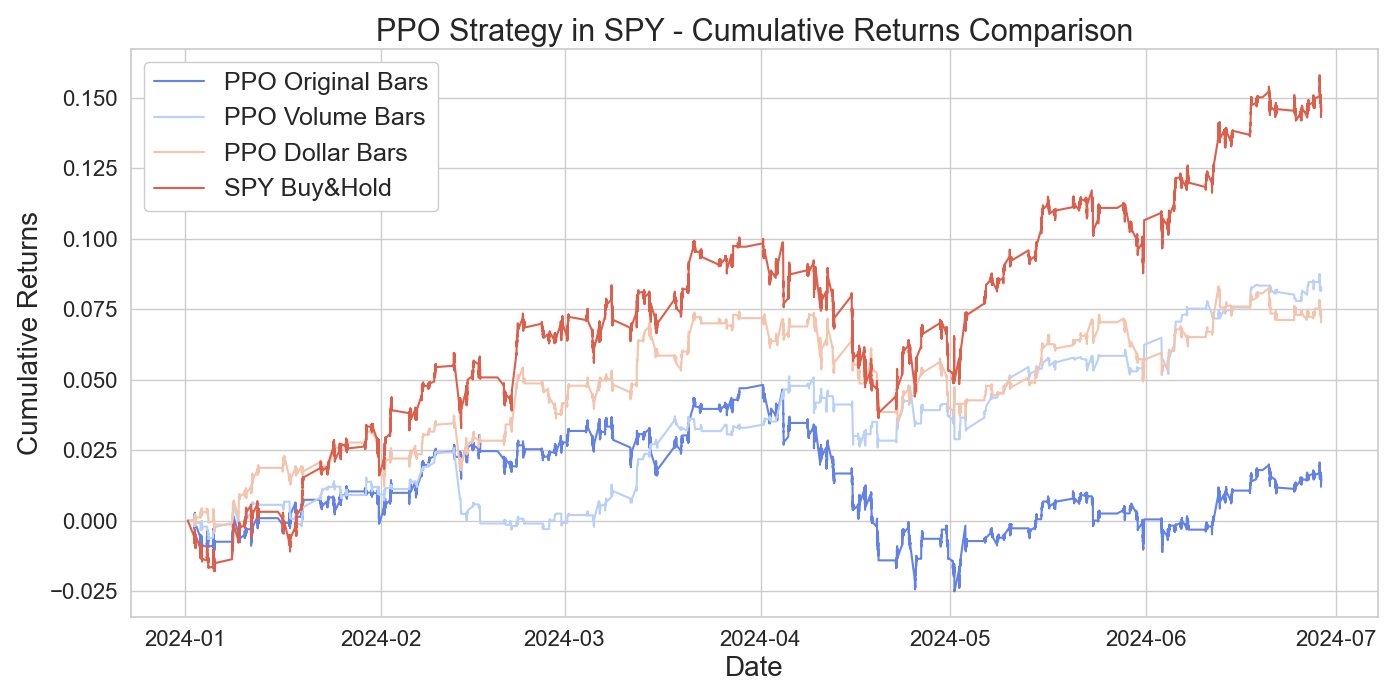
\includegraphics[width=0.6\textwidth]{./figures/ppo_spy_strategy_comparison.png}
        \caption{Comparativa de retornos acumulados de la estrategia PPO sobre SPY}
        \label{fig:ppo_spy_cum_returns_comparison}
    \end{figure}
  
    \begin{table}[h]
        \centering
        \begin{tabular}{|>{\centering\arraybackslash}m{3cm}|c|c|c|c|c|c|c|c|c|}
        \hline
        & \makecell{\textbf{Cumulative} \\ \textbf{Returns}} & \makecell{\textbf{Annualized} \\ \textbf{Return}} & \makecell{\textbf{Sharpe} \\ \textbf{Ratio}} & \makecell{\textbf{Sortino} \\ \textbf{Ratio}} & \makecell{\textbf{Maximum} \\ \textbf{Drawdown}} & \makecell{\textbf{Calmar} \\ \textbf{Ratio}} & \makecell{\textbf{Value at} \\ \textbf{Risk (VaR)}} & \textbf{Alpha} & \textbf{Beta} \\ \hline
        \makecell{\textbf{Benchmark} \\ \textbf{(S\&P 500)}} & \textbf{0.146} & \textbf{0.211} & 0.130 & 0.186 & -0.058 & 3.626 & -0.001 & 0.000 & 1.000 \\ \hline
        \makecell{\textbf{PPO Original} \\ \textbf{Bars}} & 0.015 & 0.021 & 0.019 & 0.028 & 0.070 & 0.295 & -0.000 & -0.000 & 0.632 \\ \hline
        \makecell{\textbf{PPO Volume} \\ \textbf{Bars}} & 0.082 & 0.118 & \textbf{0.473} & 0.655 & -0.028 & 4.168 & -0.001 & -0.002 & 0.356 \\ \hline
        \makecell{\textbf{PPO Dollar} \\ \textbf{Bars}} & 0.072 & 0.103 & 0.219 & 0.310 & -0.037 & 2.812 & -0.001 & -0.000 & 0.454 \\ \hline
        \end{tabular}
        \caption{Resultados de los experimentos de PPO en diferentes tipos de barras comparados con el Benchmark (SPY).}
        \label{tab:ppo_spy_results}
    \end{table}

    
    \begin{figure}[H]
        \centering
        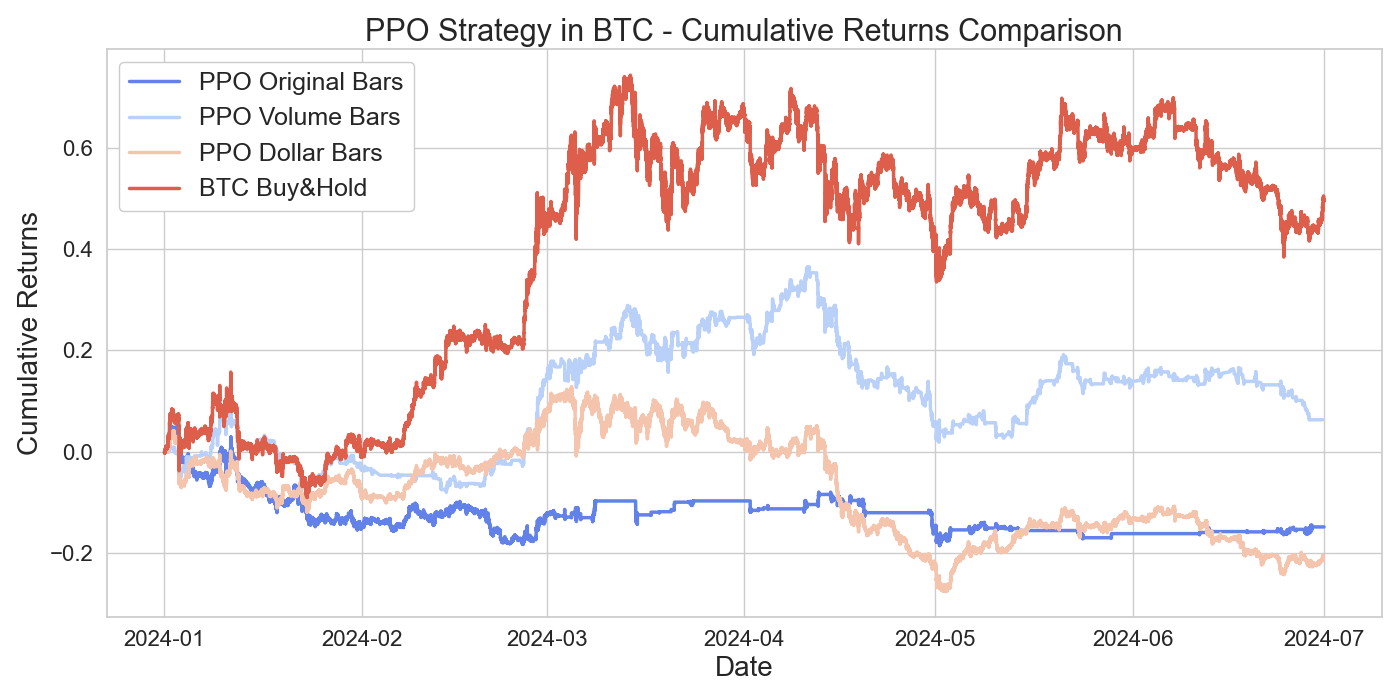
\includegraphics[width=0.6\textwidth]{./figures/ppo_btc_strategy_comparison.png}
        \caption{Comparativa de retornos acumulados de la estrategia PPO sobre BTC}
        \label{fig:ppo_btc_cum_returns_comparison}
    \end{figure}
  

    \begin{table}[h]
        \centering
        \begin{tabular}{|>{\centering\arraybackslash}m{3cm}|c|c|c|c|c|c|c|c|c|}
        \hline
        & \makecell{\textbf{Cumulative} \\ \textbf{Returns}} & \makecell{\textbf{Annualized} \\ \textbf{Return}} & \makecell{\textbf{Sharpe} \\ \textbf{Ratio}} & \makecell{\textbf{Sortino} \\ \textbf{Ratio}} & \makecell{\textbf{Maximum} \\ \textbf{Drawdown}} & \makecell{\textbf{Calmar} \\ \textbf{Ratio}} & \makecell{\textbf{Value at} \\ \textbf{Risk (VaR)}} & \textbf{Alpha} & \textbf{Beta} \\ \hline
        \makecell{\textbf{Benchmark} \\ \textbf{(BTC)}} & \textbf{0.497} & \textbf{0.753} & 0.034 & 0.048 & -0.234 & 3.216 & -0.001 & 0.000 & 1.000 \\ \hline
        \makecell{\textbf{PPO Original} \\ \textbf{Bars}} & -0.148 & -0.200 & -0.020 & -0.028 & -0.226 & -0.888 & -0.001 & -0.000 & 0.209 \\ \hline
        \makecell{\textbf{PPO Volume} \\ \textbf{Bars}} & 0.063 & 0.089 & \textbf{0.054} & 0.075 & -0.254 & 0.351 & -0.004 & -0.002 & 0.415 \\ \hline
        \makecell{\textbf{PPO Dollar} \\ \textbf{Bars}} & -0.213 & -0.284 & -0.025 & -0.034 & -0.358 & -0.792 & -0.001273 & -0.001 & 0.484 \\ \hline
        \end{tabular}
        \caption{Resultados de los experimentos de PPO en diferentes tipos de barras comparados con el Benchmark (SPY).}
        \label{tab:ppo_btc_results}
    \end{table}

  
\end{uselscape}









\chapter{Meta-labeling}

\section{Concepto y Definición de Meta-Labeling}


El \textit{Meta-Labeling} es una técnica avanzada que ha demostrado ser particularmente útil
en la creación de estrategias de trading robustas, especialmente en el contexto del aprendizaje
automático y la gestión de riesgos. 

Este método consiste en la superposición de una capa
adicional de análisis sobre una decisión de trading ya existente, evaluando la probabilidad 
de éxito de las señales generadas por un modelo base. En lugar de limitarse
a una sola predicción binaria (por ejemplo, comprar o no comprar un activo), el Meta-
Labeling aplica una segunda etapa de modelado para determinar si la señal inicial tiene
una alta probabilidad de ser correcta. Este enfoque permite refinar la decisión final,
mitigando riesgos y mejorando el rendimiento general del modelo de trading.

El proceso típico de Meta-Labeling involucra dos modelos:
\begin{enumerate}
    \item \textbf{Modelo Primario ($\mathcal{M}_1$)}: Este modelo genera la señal de 
    trading.
    \item \textbf{Meta-Modelo ($\mathcal{M}_2$)}: El meta-modelo se entrena para 
    predecir la fiabilidad de las señales generadas por el modelo primario. A cada 
    señal generada por $\mathcal{M}_1$ se le asigna un \textit{meta-label}, que 
    indica si dicha señal resultó en una operación exitosa o fallida.
\end{enumerate}

Formalmente, para una observación $i$, el modelo primario $\mathcal{M}_1$ genera 
una predicción $\hat{y}_i \in \{-1, 0, 1\}$. El meta-label $z_i \in \{0, 1\}$ se 
define de la siguiente manera:

\begin{equation}
z_i = \begin{cases} 
1 & \text{si la operación resultante de la señal } \hat{y}_i \text{ fue exitosa}, \\
0 & \text{si la operación resultante de la señal } \hat{y}_i \text{ falló}.
\end{cases},
\end{equation}

Aquí, $z_i = 1$ indica que la señal emitida por $\mathcal{M}_1$ fue confiable y 
resultó en una operación exitosa (por ejemplo, una ganancia), mientras que $z_i = 0$ 
indica que la señal no fue confiable y resultó en una operación fallida (por ejemplo, 
una pérdida).

El meta-modelo $\mathcal{M}_2$ se entrena utilizando las mismas características 
$\mathbf{x}_i$ que alimentan al modelo primario, así como la señal generada por 
$\mathcal{M}_1$, y otros indicadores adicionales que no fueron utilizados en el
modelo primario. Estos indicadores adicionales pueden incluir variables exógenas 
o nuevas características que ayuden a mejorar la capacidad del meta-modelo para 
evaluar la fiabilidad de las señales originales.

Esta estructura de dos niveles ofrece una ventaja significativa, ya que permite 
refinar las decisiones de trading al evaluar de manera más precisa la 
probabilidad de éxito de las señales iniciales. El Meta-Labeling, por tanto, 
no solo añade una capa de seguridad al proceso de toma de decisiones, sino 
que también mejora la precisión y el rendimiento general de la estrategia de trading.

\begin{figure}[H]
    \centering
    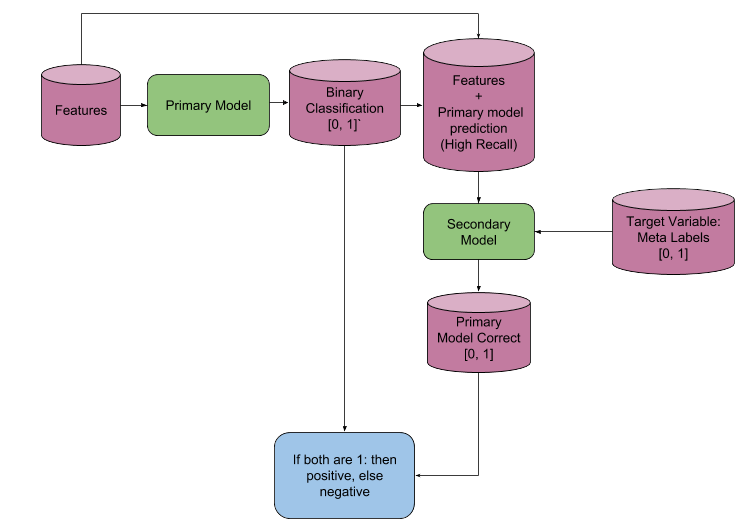
\includegraphics[width=0.9\textwidth]{./figures/meta_labeling.png}
    \caption{Diagrama Meta-Labeling (Adaptación de \textit{Hudson and Thames})}
    \label{fig:meta_labeling_diagram}
\end{figure}

Uno de los principales beneficios del Meta-Labeling es su capacidad para mejorar 
el rendimiento de un predictor que, por sí solo, puede no ser suficientemente 
robusto \cite{does_meta_labeling_add}. Supongamos que $\mathcal{M}_1$ es un modelo 
primario con una precisión moderada y un \textit{recall} bajo, lo que significa que 
emite muchas señales incorrectas (falsos positivos). Al aplicar Meta-Labeling, se 
puede ajustar el \textit{recall} y la precisión, ya que $\mathcal{M}_2$ filtra las 
señales generadas por $\mathcal{M}_1$, reduciendo el número de falsos positivos.

El rendimiento de un modelo de clasificación se evalúa comúnmente mediante métricas 
como la precisión y el \textit{recall}. Para un modelo primario $\mathcal{M}_1$, 
estas métricas se definen como:
\[
\text{Precisión} = \frac{\text{TP}}{\text{TP} + \text{FP}}, \quad \text{Recall} = \frac{\text{TP}}{\text{TP} + \text{FN}},
\]
donde TP, FP y FN son verdaderos positivos, falsos positivos y falsos negativos, 
respectivamente. Si $\mathcal{M}_1$ genera muchas señales falsas (altos FP), 
la precisión disminuye, lo que puede llevar a decisiones de trading no óptimas.

El Meta-Labeling se propone como una solución a este problema. Al entrenar 
$\mathcal{M}_2$ para predecir la probabilidad de éxito de las señales de 
$\mathcal{M}_1$, es posible aumentar la precisión del sistema general. Esto 
se debe a que $\mathcal{M}_2$ actúa como un filtro adicional que reduce los 
FP, manteniendo o incluso mejorando el \textit{recall}:
\[
\text{Precisión}_{\text{Meta}} = \frac{\text{TP}_{\text{Meta}}}{\text{TP}_{\text{Meta}} + \text{FP}_{\text{Meta}}}, \quad \text{Recall}_{\text{Meta}} = \frac{\text{TP}_{\text{Meta}}}{\text{TP}_{\text{Meta}} + \text{FN}_{\text{Meta}}},
\]
donde $\text{TP}_{\text{Meta}}$, $\text{FP}_{\text{Meta}}$, y $\text{FN}_{\text{Meta}}$ 
son los valores ajustados después de aplicar el Meta-Labeling.


\subsection{Optimización del Ratio de Sharpe mediante Meta-Labeling}

Uno de los aspectos más destacados del Meta-Labeling es su capacidad para optimizar el 
ratio de Sharpe de una estrategia de trading, mejorando el rendimiento ajustado al riesgo. 


En su forma más general, el ratio de Sharpe se define como la razón entre el exceso 
de retorno de una inversión sobre la tasa libre de riesgo y la desviación estándar 
de esos retornos. Sin embargo, en el contexto de resultados binarios, como en las 
estrategias de trading donde las decisiones se reducen a "ganar" o "perder", el ratio 
de Sharpe puede adaptarse utilizando la siguiente fórmula, tal como se describe en 
\textit{Advances in Financial Machine Learning} 
de Marcos López de Prado:

\begin{equation}
\theta(p, n, \pi^-, \pi^+) = \frac{(\pi^+ - \pi^-) p + \pi^-}{(\pi^+ - \pi^-) \sqrt{p \cdot (1 - p)}} \cdot \sqrt{n},
\end{equation}

Donde:
\begin{itemize}
    \item $\pi^+$ es el retorno asociado a un resultado positivo.
    \item $\pi^-$ es el retorno asociado a un resultado negativo.
    \item $p$ es la probabilidad de obtener un resultado positivo, es decir, la 
    probabilidad de que una operación sea exitosa.
    \item $n$ es el número de resultados o decisiones (como el número de 
    operaciones realizadas en un año).
\end{itemize}

Esta fórmula captura el rendimiento ajustado al riesgo en situaciones donde las 
decisiones de trading producen resultados binarios. La diferencia $\pi^+ - \pi^-$ 
representa el diferencial entre el retorno positivo y el negativo, que se ajusta 
por la volatilidad de los resultados, medida como $\sqrt{p \cdot (1 - p)}$. Esto 
refleja la incertidumbre inherente al sistema, basada en la probabilidad de un 
resultado positivo y la frecuencia de las operaciones.
Un valor alto de $\theta$ indica que la estrategia tiene un buen rendimiento 
relativo al riesgo asumido.



\subsection{Impacto del Meta-Labeling en el Ratio de Sharpe}

El Meta-Labeling puede jugar un papel crucial en la optimización de $\theta$. Cuando 
las ganancias ($\pi^+$) son significativamente menores que las pérdidas ($\pi^- \ll -\pi^+$), 
el ratio de Sharpe tiende a ser bajo, lo que refleja una estrategia con un rendimiento 
ajustado al riesgo desfavorable. En este caso, una forma efectiva de 
mejorar $\theta$ es aumentando la probabilidad de éxito $p$, aunque a costa de 
reducir el número de operaciones $n$. Aquí es donde entra en juego el Meta-Labeling.

\begin{itemize}
    \item \textbf{Modelo Primario ($\mathcal{M}_1$)}: El modelo primario es responsable de identificar 
    las señales iniciales de trading, determinando los posibles retornos $\pi^-$ y $\pi^+$. Sin embargo, 
    este modelo podría generar un número significativo de falsos positivos, lo que reduciría $p$ y, en 
    consecuencia, el ratio de Sharpe.
    
    \item \textbf{Meta-Modelo ($\mathcal{M}_2$)}: El modelo secundario se encarga de ajustar el umbral 
    de aceptación para filtrar las señales generadas por el modelo primario. Este modelo tiene la 
    capacidad de incrementar $p$ seleccionando solo las señales con mayor probabilidad de éxito, 
    lo que reduce el número total de operaciones $n$, pero mejora la calidad de las mismas.
\end{itemize}

Por lo tanto, el Meta-Labeling puede mejorar \(\theta\) de las siguientes maneras:

\begin{itemize}
    \item \textbf{Mejora de la Probabilidad de Éxito ($p$)}: Al aplicar Meta-Labeling, 
    se ajusta el umbral de aceptación de las señales generadas por el modelo primario. 
    Al filtrar las señales para seleccionar solo aquellas con una mayor probabilidad 
    de éxito, el Meta-Labeling aumenta $p$, mejorando así el retorno ponderado promedio en el 
    numerador de la fórmula.
    
    \item \textbf{Reducción del Riesgo (\(\sqrt{p \cdot (1 - p)}\))}: Al incrementar \(p\), 
    se reduce la variabilidad de los resultados, lo que disminuye el riesgo relativo (representado 
    por el denominador de la fórmula). Esto significa que las operaciones seleccionadas son menos 
    propensas a ser erráticas, lo que estabiliza el rendimiento de la estrategia.
    
    \item \textbf{Ajuste del Número de Operaciones ($n$)}: Aunque el número de operaciones puede 
    disminuir (menor $n$), las que se realizan tienen una mayor calidad y probabilidad de éxito. 
    Como \(n\) aparece fuera de la raíz cuadrada en la fórmula, un menor número de operaciones de 
    alta calidad puede tener un impacto significativo en la mejora del ratio de Sharpe.
\end{itemize}


Por ejemplo, si una estrategia inicialmente genera muchas señales de trading, 
pero con un alto riesgo de pérdidas, el Meta-Labeling puede reducir estas señales 
seleccionando solo aquellas con alta probabilidad de éxito, lo que resulta en menos 
operaciones, pero más seguras. Esto no solo mejora la precisión y el \textit{recall} 
de la estrategia, sino que también optimiza el ratio de Sharpe al evitar grandes 
pérdidas y mejorar el rendimiento ajustado al riesgo.

En resumen, el Meta-Labeling permite que una estrategia de trading mejore tanto en 
términos de rendimiento como de estabilidad, maximizando las ganancias relativas al 
riesgo asumido. Esta técnica es especialmente valiosa en contextos donde es crucial 
evitar grandes pérdidas y maximizar la probabilidad de éxito de las 
operaciones \cite{lopezdeprado2018afml}.


\subsubsection{Beneficios del F1-Score y del Control de Tamaño de las Apuestas}

El Meta-Labeling es particularmente útil para lograr mayores \textit{F1-scores}. 
Primero, se construye un modelo que logre un alto \textit{recall}, incluso si la 
precisión no es particularmente alta. Luego, se corrige la baja precisión aplicando 
Meta-Labeling a los positivos identificados por el modelo primario. Esto permite 
obtener un \textit{F1-score} más equilibrado y un modelo más robusto en la 
identificación de oportunidades de trading.

Además, el Meta-Labeling permite desarrollar un sistema de ML que, en lugar de 
ser una caja negra, actúa como una caja blanca, en la que se puede entender y 
ajustar la lógica detrás de las decisiones tomadas. Esto es crucial para limitar 
los efectos del sobreajuste, ya que el ML no decide el lado de la apuesta, sino 
solo el tamaño de la misma. En este sentido, el Meta-Labeling permite gestionar 
adecuadamente el tamaño de las apuestas, evitando situaciones en las que se 
logre alta precisión en pequeñas apuestas, pero baja precisión en apuestas 
grandes, lo que podría llevar a la ruina \cite{lopezdeprado2018afml}.


\section{Etiquetado de Datos Financieros}

Para aplicar Meta-Labeling de manera efectiva, es imprescindible etiquetar correctamente 
los datos financieros. El etiquetado de datos consiste en asignar una etiqueta a cada 
señal de trading que indique si la operación resultante fue exitosa o fallida. 

Este proceso es crucial, ya que el etiquetado correcto de las señales es lo que 
permitirá al meta-modelo aprender y predecir la fiabilidad de futuras señales 
emitidas por el modelo primario.

\subsection{Método del Horizonte Temporal Fijo}

El \textit{método del horizonte temporal fijo} es una técnica ampliamente utilizada en la literatura financiera para etiquetar datos. Este método asigna etiquetas a las observaciones basándose en el retorno del activo durante un período de tiempo predefinido después de que se genera una señal de trading.

\subsubsection{Descripción del Método}

Consideremos:

\begin{itemize}
    \item Una matriz de características $\mathbf{X}$ con $I$ filas, donde cada fila representa una observación $\mathbf{X}_i$ correspondiente a un instante temporal $t$.
    \item Un umbral fijo $\tau$ que define la magnitud mínima del retorno necesaria para considerar una operación como exitosa o fallida.
    \item Un horizonte temporal fijo $h$, que representa el número de barras de tiempo que se observan después de la generación de la señal.
\end{itemize}

El procedimiento de etiquetado se define de la siguiente manera:

\begin{enumerate}
    \item \textbf{Generación de la Señal}: En el tiempo $t_{i,0}$, inmediatamente después de observar $\mathbf{X}_i$, se genera una señal de trading.
    \item \textbf{Cálculo del Retorno}: Se calcula el retorno del precio del activo desde $t_{i,0}$ hasta $t_{i,0} + h$ mediante la siguiente expresión:
    \begin{equation}
        r_{t_{i,0}, t_{i,0}+h} = \frac{P_{t_{i,0}+h}}{P_{t_{i,0}}} - 1,
    \end{equation}
    donde $P_t$ representa el precio del activo en el tiempo $t$.
    \item \textbf{Asignación de Etiquetas}: La etiqueta $y_i$ se asigna según el valor de $r_{t_{i,0}, t_{i,0}+h}$ comparado con el umbral $\tau$:
    \begin{equation}
        y_i = 
        \begin{cases} 
            1 & \text{si } r_{t_{i,0}, t_{i,0}+h} > \tau, \\
            -1 & \text{si } r_{t_{i,0}, t_{i,0}+h} < -\tau, \\
            0 & \text{si } |r_{t_{i,0}, t_{i,0}+h}| \leq \tau.
        \end{cases}
    \end{equation}
\end{enumerate}


A pesar de su simplicidad y amplia adopción, este método presenta varias limitaciones importantes:

\begin{enumerate}
    \item \textbf{Ignorancia de la Volatilidad Variable}: El uso de un umbral fijo $\tau$ 
    no considera que la volatilidad del mercado puede variar significativamente en diferentes 
    momentos. Por ejemplo, durante períodos de alta volatilidad, un umbral $\tau$ puede 
    ser demasiado bajo, etiquetando muchas observaciones como positivas o negativas de 
    manera inapropiada. Contrariamente, durante períodos de baja volatilidad, el mismo 
    umbral puede ser demasiado alto, resultando en la mayoría de las observaciones 
    etiquetadas como neutrales.
    
    \item \textbf{Desconsideración de la Ruta de Precios}: El método solo considera el 
    precio inicial y final dentro del horizonte temporal, ignorando el camino seguido 
    por el precio entre estos puntos.Esto es problemático porque en la práctica, las 
    estrategias de trading están sujetas a niveles de \textit{stop-loss} y 
    \textit{take-profit} que pueden activarse antes de que finalice el horizonte temporal.
    Ignorar estos eventos intermedios puede llevar a etiquetados engañosos que no reflejan 
    las condiciones reales de mercado y gestión de riesgo.

    \item \textbf{Dependencia de Barras de Tiempo}: El método se basa en barras de tiempo 
    fijas, que pueden no capturar adecuadamente la actividad del mercado, especialmente 
    en activos con volúmenes de negociación variables. Esto puede resultar en una 
    representación inconsistente de la información del mercado y afectar negativamente 
    la calidad del etiquetado.

\end{enumerate}

Estas limitaciones pueden conducir a un etiquetado inexacto y, por lo tanto, afectar 
la capacidad del modelo para aprender y predecir efectivamente.

\subsection{Método de las Tres Barreras}

El \textit{Método de las Tres Barreras} (\textit{Three-Barrier Method}) es una 
técnica alternativa de etiquetado que proporciona una mayor precisión que el 
método del horizonte temporal fijo, especialmente en entornos de trading donde 
la ruta seguida por el precio, así como los niveles de \textit{stop-loss} y 
\textit{take-profit}, son fundamentales.

Este método consiste en definir tres barreras que determinan cómo se etiqueta 
una observación en función de cuál de ellas es alcanzada primero. Las barreras 
son las siguientes:

\begin{itemize}
    \item \textbf{Barrera Superior (\textit{Take Profit})}: Representa un nivel 
    de precio predefinido que, si se alcanza, indica que la operación ha sido 
    exitosa. En este caso, se asigna una etiqueta de $y_i = 1$.
    \item \textbf{Barrera Inferior (\textit{Stop-Loss})}: Es un nivel de 
    precio que, si se toca primero, indica que la operación ha fallado, por lo 
    que se asigna una etiqueta de $y_i = -1$.
    \item \textbf{Barrera Temporal (\textit{Expiration Limit})}: Define el número 
    máximo de barras de tiempo después de las cuales se fuerza el cierre de la
    operación, independientemente de si se ha alcanzado alguna de las otras dos 
    barreras. Si se toca esta barrera antes que las otras, se puede asignar 
    una etiqueta de $y_i = 0$, o bien, según la preferencia, se puede etiquetar 
    en función del signo del retorno acumulado hasta ese momento.
\end{itemize}

\textbf{Figura~\ref{fig:three_barrier_method}} ilustra cómo funcionan estas tres 
barreras. En la imagen, se observa un ejemplo de trayectoria del precio donde las 
barreras determinan el etiquetado de la señal:

\begin{figure}[H]
    \centering
    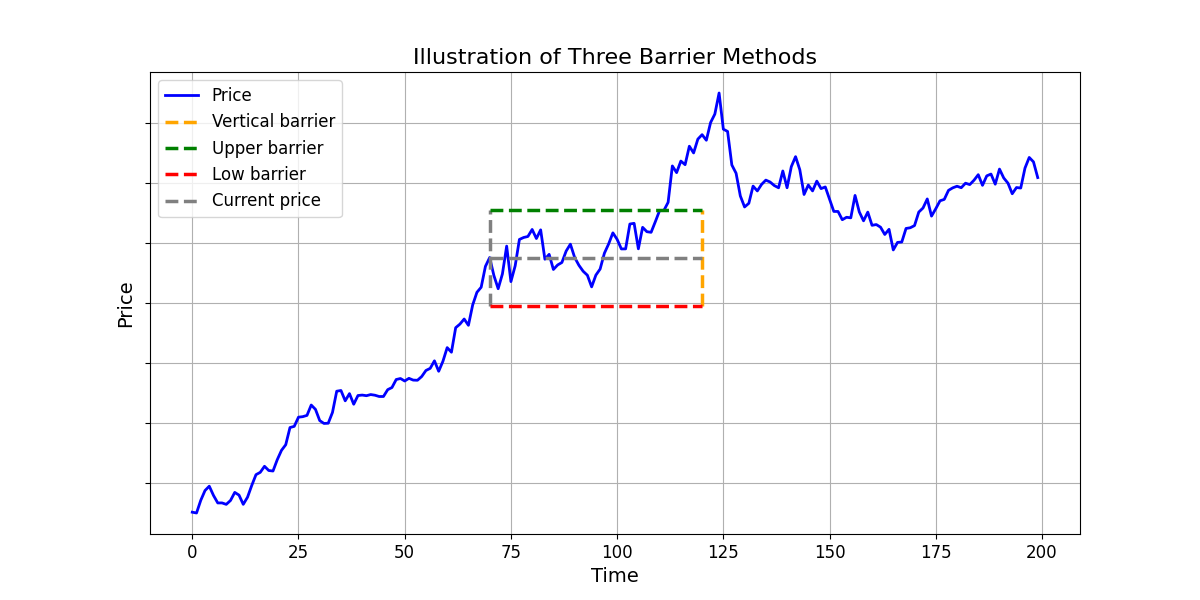
\includegraphics[width=1\textwidth]{./figures/three_barried_method.png}
    \caption{Ilustración del método de las trés barreras}
    \label{fig:three_barrier_method}
\end{figure}

A diferencia del método del horizonte temporal fijo, el \textit{Three-Barrier Method} 
es dependiente de la ruta (\textit{path-dependent}), lo que significa que toma en cuenta 
toda la trayectoria del precio desde el momento en que se genera la señal ($t_{i,0}$) 
hasta que se toca una de las barreras. 

Este método permite etiquetar de manera más realista las operaciones, ya que considera 
tanto los límites de toma de ganancias y pérdidas como un límite temporal, proporcionando 
una visión más completa del comportamiento del precio.

Este enfoque también ofrece varias ventajas clave. En primer lugar, al considerar 
dinámicamente los niveles de toma de ganancias y stop-loss, que pueden ajustarse en 
función de la volatilidad, el método reduce la probabilidad de etiquetar incorrectamente 
las observaciones. Esto es especialmente importante en mercados volátiles, donde los 
precios pueden fluctuar considerablemente en cortos períodos de tiempo. Además, 
la inclusión de una barrera temporal introduce una capa adicional de control, 
permitiendo cerrar una operación si no se alcanzan ni el nivel de toma de ganancias 
ni el de pérdidas dentro del tiempo estipulado, lo que ayuda a evitar situaciones en 
las que se mantenga una posición de manera indefinida sin obtener un beneficio claro.

En resumen, el \textit{Método de las Tres Barreras} no solo mejora la precisión del 
etiquetado al tener en cuenta toda la ruta del precio, sino que también proporciona 
un mecanismo más flexible y adaptativo para la gestión de operaciones en estrategias 
de trading. Al combinar estos elementos, este método contribuye significativamente a 
la creación de estrategias de trading más robustas y efectivas, optimizando el 
rendimiento ajustado al riesgo en un entorno financiero incierto.

\section{Implementación de Meta-Labeling en Trading Algorítmico}

Para la obtención de las etiquetas base (\textit{labels}), que 
son fundamentales para evaluar las señales generadas por el modelo primario, se han 
desarrollado una serie de funciones que procesan los datos históricos de precios.

A continuación, se describen brevemente las funciones desarrolladas:

\begin{itemize}
    
    \item \texttt{calculate\_rolling\_volatility}: Calcula la volatilidad móvil de 
    los precios de cierre, utilizando una media móvil ponderada exponencialmente (EWMA). 
    Esta volatilidad es esencial para definir los umbrales de \textit{stop loss} y 
    \textit{take profit}.
    
    \item \texttt{get\_horizons}: Determina los horizontes temporales futuros en 
    los que se evalúan las señales de trading. Define el tiempo máximo (en minutos) 
    para que un evento de \textit{stop loss} o \textit{take profit} ocurra.
    
    \item \texttt{get\_touches}: Calcula los puntos en el tiempo donde los precios 
    tocan los niveles de \textit{stop loss} y \textit{take profit}, según los 
    umbrales definidos por la volatilidad móvil.
    
    \item \texttt{get\_labels}: Asigna las etiquetas finales a las señales de 
    trading basándose en los resultados de las funciones anteriores. Define si 
    una señal es exitosa (\textit{take profit}), fallida (\textit{stop loss}), 
    o neutra.

    \item \texttt{process\_ohlc\_data}: Procesa los datos OHLC (Open, High, Low, 
    Close) para generar etiquetas de eventos mediante la orquestación del resto 
    de funciones.
    
\end{itemize}


Las etiquetas base (\textit{labels}) se generan evaluando el comportamiento de las 
señales de trading en relación con la volatilidad diaria y un horizonte temporal 
predefinido. La volatilidad diaria, calculada mediante la función 
\texttt{calculate\_rolling\_volatility}, se utiliza para establecer los umbrales 
que determinan si una señal es exitosa o fallida. Cuando una señal supera el 
umbral superior definido por la volatilidad móvil diaria, se le asigna la 
etiqueta \textbf{1} (\textit{take profit}). Si, por el contrario, la señal cae 
por debajo del umbral inferior, se etiqueta como \textbf{-1} (\textit{stop loss}).

Para aquellas señales que no alcanzan ni el límite superior ni el inferior dentro 
de un horizonte temporal específico, se utiliza la función \texttt{get\_horizons}, 
que asigna la etiqueta \textbf{0}. Este horizonte temporal se ha fijado en un 
periodo de 5 días, equivalente a 7200 minutos (\texttt{60*24*5}).

Finalmente, la función \texttt{get\_labels} consolida estas decisiones, asignando 
la etiqueta correspondiente a cada muestra de datos. Así, las etiquetas base 
reflejan con precisión el comportamiento de las señales en función de los umbrales 
de volatilidad y los horizontes temporales establecidos.

Una vez obtenidas las etiquetas base (\textit{labels}) para las señales de trading, se procede a la creación de los \textit{meta-labels}. Los \textit{meta-labels} se generan al comparar las señales predichas por el modelo primario de trading con las etiquetas base:

\begin{itemize}
    \item Si la señal predicha por el modelo coincide con la etiqueta base (\textit{label} = 1 o \textit{label} = -1), el \textit{meta-label} se asigna como \textbf{1}, indicando un éxito.
    \item Si la señal predicha por el modelo no coincide con la etiqueta base o si la etiqueta base es 0, el \textit{meta-label} se asigna como \textbf{0}, indicando un fracaso.
\end{itemize}

De esta manera, los \textit{meta-labels} se utilizan como la variable respuesta (\textit{y}) en el proceso de entrenamiento del modelo de \textit{XGBoost}.

\subsection{Conjunto de Datos de Entrenamiento (\textit{X})}

El conjunto de datos de entrada (\textit{X}) para el modelo \textit{XGBoost} se conforma a 
partir de varias fuentes:

\begin{itemize}
    \item \textbf{Datos originales de mercado}: Datos originales de mercado utilizados para 
    el entrenamiento del modelo \textit{PPO} presentados en la Sección \ref{sec:espacio_observaciones}.
    \item \textbf{Señales del modelo primario}: Señales generadas por el modelo 
    principal de trading que indican puntos de entrada o salida en el mercado, $\mathcal{A} = \{-1, 0, 1\}$.
    \item \textbf{Indicador basado en cadenas de Markov}: Las cadenas de Markov ocultas 
    (\textit{Hidden Markov Models}, HMM) son modelos estadísticos que permiten describir 
    un sistema que cambia de estado de manera probabilística. En el contexto de series 
    temporales financieras, un \textit{HMM} puede identificar diferentes regímenes del 
    mercado, que corresponden a distintos patrones de comportamiento en los precios, 
    como fases de alta volatilidad o de mercado estable. Cada régimen se define como 
    un estado oculto en la cadena de Markov, y las transiciones entre estados se 
    modelan en función de probabilidades. Este indicador se introduce como un 
    componente adicional en el conjunto de datos de entrada (\textit{X}).
    
\end{itemize}

Una vez entrenado el modelo de \textit{XGBoost} utilizando los \textit{meta-labels} como 
variable respuesta, se utiliza el modelo para realizar predicciones sobre el conjunto de 
datos \textit{out-of-sample}. 


\section{Evaluación del Modelo y Resultados}

Una vez entrenado el modelo \textit{XGBoost} con los \textit{meta-labels}, se utiliza para realizar 
predicciones sobre el conjunto de datos \textit{out-of-sample}. Estas predicciones se emplean para 
filtrar las señales generadas por el modelo primario. El proceso de filtrado es sencillo: si la 
predicción del \textit{meta-label} es 1, la señal del modelo primario prevalece; en caso contrario, 
la señal es descartada.

Este enfoque permite mejorar la robustez de las decisiones de trading, asegurando que solo se 
consideren aquellas señales que han sido validadas por el proceso de \textit{meta-labeling}. Para 
evaluar el impacto de este filtro, se comparan las señales del modelo primario con los \textit{labels} 
obtenidos mediante la técnica \textit{Three Barrier Method} en el conjunto de 
datos \textit{out-of-sample}, tanto antes como después de aplicar el \textit{meta-labeling}.

Es importante señalar que, debido a las limitaciones computacionales y el tiempo necesario para 
procesar el gran volumen de datos, no fue posible generar las señales del modelo primario sobre el 
conjunto de datos \textit{in-sample} para los datos originales de BTC. Por esta razón, los 
resultados correspondientes a este caso no se presentan en este análisis.

Las métricas de evaluación se presentan en forma de un reporte de clasificación multiclase, donde 
las clases son -1, 0, y 1. Este reporte permite analizar el desempeño del modelo en términos de 
\textit{precision}, \textit{recall} y \textit{f1-score}, para cada una de las clases, 
así como la \textit{accuracy} general del modelo. A continuación, se muestran las comparativas 
para los diferentes conjuntos de datos, antes y después de aplicar el \textit{meta-labeling}.


\begin{table}[h!]
    \centering
    \begin{tabular}{lccccc}
    \hline
    \textbf{Clase} & \textbf{Métrica} & \textbf{Antes (BTC Dollar)} & \textbf{Después (BTC Dollar)} \\
    \hline
    \multirow{3}{*}{\textbf{-1.0}} & \textbf{Precision} & 0.48 & 0.48 \\
                                   & \textbf{Recall}    & 0.30 & 0.24 \\
                                   & \textbf{F1-Score}  & 0.37 & 0.32 \\
                                   & \textbf{Support}   & 76435 & 76435 \\
    \hline
    \multirow{3}{*}{\textbf{0.0}} & \textbf{Precision}  & 0.00 & 0.00 \\
                                  & \textbf{Recall}     & 0.48 & 0.73 \\
                                  & \textbf{F1-Score}   & 0.00 & 0.00 \\
                                  & \textbf{Support}    & 52 & 52 \\
    \hline
    \multirow{3}{*}{\textbf{1.0}} & \textbf{Precision}  & 0.52 & 0.54 \\
                                  & \textbf{Recall}     & 0.34 & 0.09 \\
                                  & \textbf{F1-Score}   & 0.41 & 0.15 \\
                                  & \textbf{Support}    & 81919 & 81919 \\
    \hline
    \textbf{General} & \textbf{Accuracy} & 0.32 & 0.16 \\
    \hline
    \end{tabular}
    \caption{Comparación del reporte de clasificación antes y después de aplicar \textit{meta-labeling} para BTC Dollar.}
    \label{tab:classification_report_btc_dollar}
\end{table}

\begin{table}[h!]
    \centering
    \begin{tabular}{lccccc}
    \hline
    \textbf{Clase} & \textbf{Métrica} & \textbf{Antes (BTC Volume)} & \textbf{Después (BTC Volume)} \\
    \hline
    \multirow{3}{*}{\textbf{-1.0}} & \textbf{Precision} & 0.48 & 0.48 \\
                                    & \textbf{Recall}    & 0.24 & 0.15 \\
                                    & \textbf{F1-Score}  & 0.32 & 0.23 \\
                                    & \textbf{Support}   & 5503 & 5503 \\
    \hline
    \multirow{3}{*}{\textbf{0.0}} & \textbf{Precision}  & 0.00 & 0.00 \\
                                    & \textbf{Recall}     & 0.00 & 0.00 \\
                                    & \textbf{F1-Score}   & 0.00 & 0.00 \\
                                    & \textbf{Support}    & 0 & 0 \\
    \hline
    \multirow{3}{*}{\textbf{1.0}} & \textbf{Precision}  & 0.53 & 0.52 \\
                                    & \textbf{Recall}     & 0.13 & 0.06 \\
                                    & \textbf{F1-Score}   & 0.21 & 0.11 \\
                                    & \textbf{Support}    & 6066 & 6066 \\
    \hline
    \textbf{General} & \textbf{Accuracy} & 0.18 & 0.10 \\
    \hline
    \end{tabular}
    \caption{Comparación del reporte de clasificación antes y después de aplicar \textit{meta-labeling} para BTC Volume.}
    \label{tab:classification_report_btc_volume}
\end{table}
    

\begin{table}[h!]
    \centering
    \begin{tabular}{lccccc}
    \hline
    \textbf{Clase} & \textbf{Métrica} & \textbf{Antes (SPY Original)} & \textbf{Después (SPY Original)} \\
    \hline
    \multirow{3}{*}{\textbf{-1.0}} & \textbf{Precision} & 0.46 & 0.45 \\
                                   & \textbf{Recall}    & 0.25 & 0.12 \\
                                   & \textbf{F1-Score}  & 0.32 & 0.19 \\
                                   & \textbf{Support}   & 22352 & 22352 \\
    \hline
    \multirow{3}{*}{\textbf{0.0}} & \textbf{Precision}  & 0.01 & 0.01 \\
                                  & \textbf{Recall}     & 0.33 & 0.71 \\
                                  & \textbf{F1-Score}   & 0.01 & 0.01 \\
                                  & \textbf{Support}    & 326 & 326 \\
    \hline
    \multirow{3}{*}{\textbf{1.0}} & \textbf{Precision}  & 0.53 & 0.54 \\
                                  & \textbf{Recall}     & 0.40 & 0.15 \\
                                  & \textbf{F1-Score}   & 0.46 & 0.23 \\
                                  & \textbf{Support}    & 25478 & 25478 \\
    \hline
    \textbf{General} & \textbf{Accuracy} & 0.33 & 0.14 \\
    \hline
    \end{tabular}
    \caption{Comparación del reporte de clasificación antes y después de aplicar \textit{meta-labeling} para SPY Original.}
    \label{tab:classification_report_spy_original}
\end{table}
    

\begin{table}[h!]
    \centering
    \begin{tabular}{lccccc}
    \hline
    \textbf{Clase} & \textbf{Métrica} & \textbf{Antes (SPY Volume)} & \textbf{Después (SPY Volume)} \\
    \hline
    \multirow{3}{*}{\textbf{-1.0}} & \textbf{Precision} & 0.46 & 0.49 \\
                                   & \textbf{Recall}    & 0.42 & 0.18 \\
                                   & \textbf{F1-Score}  & 0.44 & 0.26 \\
                                   & \textbf{Support}   & 1540 & 1540 \\
    \hline
    \multirow{3}{*}{\textbf{0.0}} & \textbf{Precision}  & 0.01 & 0.01 \\
                                  & \textbf{Recall}     & 0.24 & 0.76 \\
                                  & \textbf{F1-Score}   & 0.01 & 0.02 \\
                                  & \textbf{Support}    & 29 & 29 \\
    \hline
    \multirow{3}{*}{\textbf{1.0}} & \textbf{Precision}  & 0.53 & 0.52 \\
                                  & \textbf{Recall}     & 0.19 & 0.09 \\
                                  & \textbf{F1-Score}   & 0.28 & 0.16 \\
                                  & \textbf{Support}    & 1847 & 1847 \\
    \hline
    \textbf{General} & \textbf{Accuracy} & 0.29 & 0.14 \\
    \hline
    \end{tabular}
    \caption{Comparación del reporte de clasificación antes y después de aplicar \textit{meta-labeling} para SPY Volume.}
    \label{tab:classification_report_spy_volume}
\end{table}
    

\begin{table}[h!]
    \centering
    \begin{tabular}{lccccc}
    \hline
    \textbf{Clase} & \textbf{Métrica} & \textbf{Antes (SPY Dollar)} & \textbf{Después (SPY Dollar)} \\
    \hline
    \multirow{3}{*}{\textbf{-1.0}} & \textbf{Precision} & 0.45 & 0.46 \\
                                   & \textbf{Recall}    & 0.31 & 0.13 \\
                                   & \textbf{F1-Score}  & 0.37 & 0.20 \\
                                   & \textbf{Support}   & 3759 & 3759 \\
    \hline
    \multirow{3}{*}{\textbf{0.0}} & \textbf{Precision}  & 0.01 & 0.01 \\
                                  & \textbf{Recall}     & 0.36 & 0.79 \\
                                  & \textbf{F1-Score}   & 0.02 & 0.02 \\
                                  & \textbf{Support}    & 67 & 67 \\
    \hline
    \multirow{3}{*}{\textbf{1.0}} & \textbf{Precision}  & 0.53 & 0.51 \\
                                  & \textbf{Recall}     & 0.39 & 0.10 \\
                                  & \textbf{F1-Score}   & 0.45 & 0.17 \\
                                  & \textbf{Support}    & 4429 & 4429 \\
    \hline
    \textbf{General} & \textbf{Accuracy} & 0.35 & 0.12 \\
    \hline
    \end{tabular}
    \caption{Comparación del reporte de clasificación antes y después de aplicar \textit{meta-labeling} para SPY Dollar.}
    \label{tab:classification_report_spy_dollar}
\end{table}
    

\section{Análisis de Resultados y Conclusiones}

Al examinar los resultados obtenidos tras la aplicación del \textit{meta-labeling}, se observa una tendencia general de 
deterioro en las métricas de rendimiento del modelo, lo cual contrasta con las expectativas iniciales de mejora. La 
comparación entre los resultados obtenidos antes y después de aplicar el \textit{meta-labeling} en los diferentes 
conjuntos de datos revela que, en la mayoría de los casos, la \textit{accuracy}, el \textit{recall} y el \textit{f1-score} 
se vieron negativamente afectados.

En el caso de BTC Dollar, se observó que, aunque la precisión para las clases -1 y 1 se mantuvo relativamente 
constante o incluso mejoró ligeramente, el \textit{recall} disminuyó significativamente. Este descenso en el \textit{recall} 
sugiere que el modelo fue menos efectivo en identificar correctamente tanto las señales positivas como negativas después de 
aplicar el \textit{meta-labeling}. Esto se traduce en una menor capacidad del modelo para aprovechar las oportunidades de 
trading o para evitar operaciones potencialmente fallidas, lo que impacta negativamente en el \textit{f1-score} general.

Una tendencia similar se observó en BTC Volume, donde la \textit{accuracy} general se redujo de 0.18 a 0.10 tras el 
\textit{meta-labeling}. En este caso, el \textit{recall} para la clase 1.0 (señales positivas) también disminuyó 
considerablemente, lo que indica que el modelo perdió eficacia al identificar correctamente las señales de éxito. 
Este resultado pone en evidencia que, aunque el \textit{meta-labeling} pretende filtrar y mejorar la calidad de las 
señales del modelo primario, en la práctica, podría estar eliminando señales que, a pesar de su menor confianza 
inicial, habrían resultado en operaciones exitosas.

Para SPY, tanto en los conjuntos de datos originales como en los basados en volumen y dólares, el \textit{meta-labeling} 
no solo no mejoró las métricas, sino que en muchos casos las empeoró. En SPY Original, la \textit{accuracy} cayó de 0.33 
a 0.14, mientras que en SPY Volume y SPY Dollar, la \textit{accuracy} también disminuyó significativamente. En particular, 
el \textit{recall} para las clases -1 y 1 se redujo notablemente en estos conjuntos de datos, lo que sugiere que el 
modelo se volvió más conservador, optando con mayor frecuencia por no realizar operaciones (clase 0), en lugar de tomar 
decisiones de trading. Esto es especialmente evidente en SPY Dollar, donde el \textit{recall} para la clase 0 aumentó de 
manera considerable, mientras que el \textit{recall} para las clases de trading activas se desplomó.

Un patrón que se repite en todas las comparaciones es la mejora generalizada en el \textit{recall} de la 
predicción de la clase 0.0 (no trade) después de aplicar el \textit{meta-labeling}, mientras que para las clases -1 y 1, 
la precisión apenas mejora, y el \textit{recall} baja considerablemente. Esto puede indicar que el modelo, tras el 
filtrado con \textit{meta-labels}, se vuelve más conservador, optando por no tomar decisiones de trading en lugar 
de arriesgarse con operaciones que podrían ser fallidas o exitosas.

Es importante destacar que los resultados obtenidos pueden estar profundamente influenciados por los hiperparámetros 
seleccionados durante la generación de los \textit{labels}. La elección de los umbrales de volatilidad, 
los horizontes temporales y otros parámetros clave tiene un impacto directo en la distribución de las clases, 
particularmente en la prevalencia de la clase 0 (no trade). En este análisis, se observó una baja proporción 
de señales etiquetadas como 0 en comparación con las clases -1 y 1, lo que sugiere que los parámetros 
elegidos han favorecido la clasificación de la mayoría de las señales como activas (trading) en lugar de neutras 
(no trade). Esta configuración puede haber agudizado el conservadurismo observado en el modelo filtrado por 
\textit{meta-labels}, ya que una menor cantidad de señales etiquetadas como 0 originalmente limita la capacidad 
del \textit{meta-labeling} para realizar un filtrado más equilibrado. Por tanto, es fundamental reconocer que la 
calibración de estos hiperparámetros es un proceso delicado, que requiere un ajuste cuidadoso para asegurar que 
el \textit{meta-labeling} aporte valor añadido al proceso de decisión.

En conjunto, estos resultados sugieren que el proceso de \textit{meta-labeling} aplicado no logró su objetivo de 
mejorar la robustez de las señales de trading. En cambio, el modelo filtrado por el \textit{meta-labeling} mostró 
una tendencia a reducir su capacidad para identificar correctamente las oportunidades de mercado, lo que resultó 
en un desempeño inferior en términos de \textit{recall} y \textit{f1-score}. Es posible que el \textit{meta-labeling} 
haya sido demasiado restrictivo, eliminando señales que, aunque inicialmente parecían menos seguras, podrían haber 
resultado en operaciones exitosas. Este análisis subraya la necesidad de revisar la metodología de \textit{meta-labeling} 
utilizada o de explorar alternativas que puedan adaptarse mejor a la naturaleza volátil y compleja de los mercados 
financieros analizados en este estudio.


\section{Resultados Finales: Rendimiento Acumulado de las Estrategias}


En las Figuras \ref{fig:final_spy_cum_returns_comparison_img} y \ref{fig:final_btc_cum_returns_comparison_img}, 
se muestran los gráficos del rendimiento acumulado de las estrategias para BTC Dollar y SPY Volume, respectivamente, 
comparando el rendimiento antes y después de aplicar el \textit{meta-labeling}. En las Tablas 
\ref{tab:final_spy_cum_returns_comparison_table} y \ref{tab:final_btc_cum_returns_comparison_table} se recogen 
las metricas principales de las estrategias, mientras que en la Tabla \ref{tab:final_returns_comparison}, 
se resumen los rendimientos finales acumulados para todos los conjuntos de datos analizados. 

  % Forzamos un salto de página
\begin{uselscape}

    \begin{figure}[H]
        \centering
        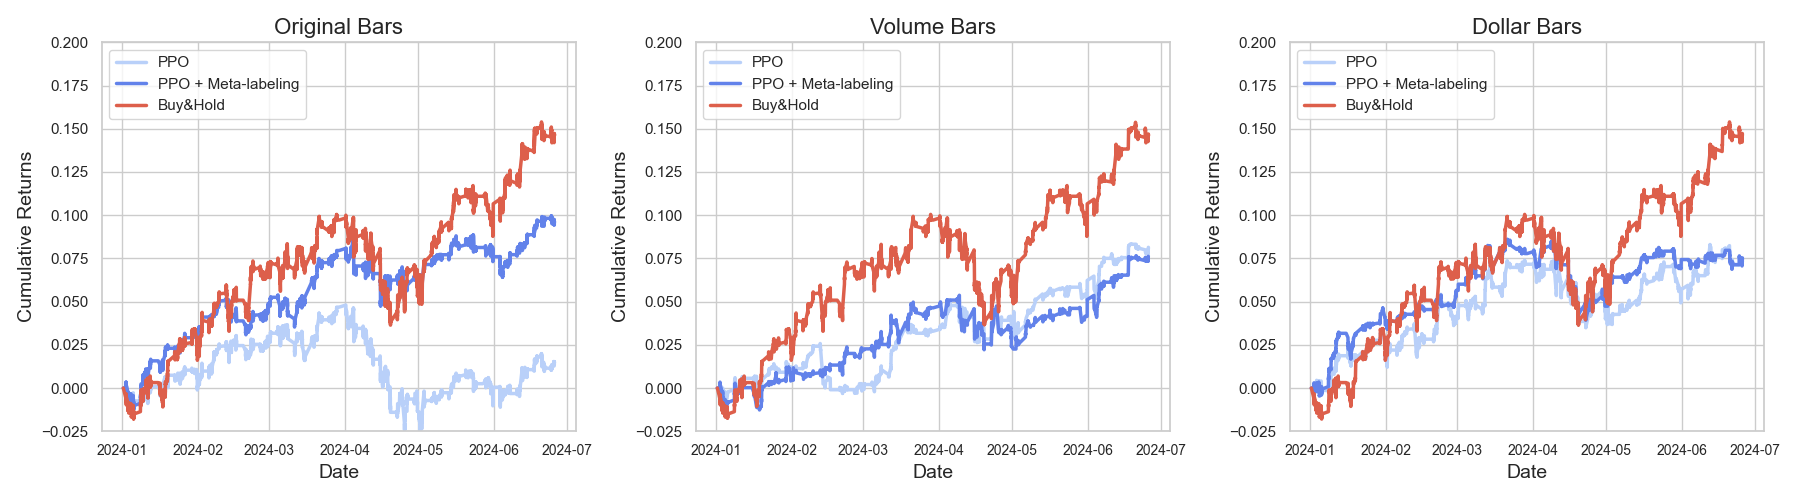
\includegraphics[width=1.05\textwidth]{./figures/final_spy_strategy_comparison_horizontal.png}
        \caption{Comparativa de retornos acumulados de la estrategia final sobre SPY}
        \label{fig:final_spy_cum_returns_comparison_img}
    \end{figure}
  
    % \begin{table}[h]
    %     \centering
    %     \begin{scriptsize}
    %     \begin{tabular}{|>{\scriptsize\centering\arraybackslash}m{4cm}|c|c|c|c|c|c|c|c|c|}
    %     \hline
    %     & \makecell{\textbf{Cumulative} \\ \textbf{Returns}} & \makecell{\textbf{Annualized} \\ \textbf{Return}} & \makecell{\textbf{Sharpe} \\ \textbf{Ratio}} & \makecell{\textbf{Sortino} \\ \textbf{Ratio}} & \makecell{\textbf{Maximum} \\ \textbf{Drawdown}} & \makecell{\textbf{Calmar} \\ \textbf{Ratio}} & \makecell{\textbf{Value at} \\ \textbf{Risk (VaR)}} & \textbf{Alpha} & \textbf{Beta} \\ \hline
    %     \makecell{\textbf{Benchmark} \\ \textbf{(S\&P 500)}} & \textbf{0.146} & \textbf{0.216} & 0.133 & 0.191 & -0.058 & 3.705 & -0.001 & 0.000 & 1.000 \\ \hline
    %     \makecell{\textbf{PPO Original} \\ \textbf{Bars}} & 0.015 & 0.021 & 0.020 & 0.028 & -0.070 & 0.300 & -0.000 & -0.000 & 0.630 \\ \hline
    %     \makecell{\textbf{PPO + Meta-labeling} \\ \textbf{Original Bars}} & 0.096 & 0.140 & 0.134 & 0.199 & -0.036 & 3.835 & -0.000 & 0.000 & 0.439 \\ \hline
    %     \makecell{\textbf{PPO Volume} \\ \textbf{Bars}} & 0.081 & 0.119 & \textbf{0.478} & \textbf{0.662} & -0.028 & 4.208 & -0.001 & 0.002 & 0.355 \\ \hline
    %     \makecell{\textbf{PPO + Meta-labeling} \\ \textbf{Volume Bars}} & 0.076 & 0.111 & 0.413 & 0.570 & -0.030 & 3.705 & -0.001 & 0.001 & 0.421 \\ \hline
    %     \makecell{\textbf{PPO Dollar} \\ \textbf{Bars}} & 0.073 & 0.107 & 0.227 & 0.322 & -0.036 & 2.928 & -0.001 & -0.000 & 0.544 \\ \hline
    %     \makecell{\textbf{PPO + Meta-labeling} \\ \textbf{Dollar Bars}} & 0.074 & 0.108 & 0.276 & 0.387 & -0.044 & 2.474 & -0.001 & 0.001 & 0.374 \\ \hline
    %     \end{tabular}
    %     \caption{Resultados del rendimiento acumulado y métricas de riesgo para PPO con y sin \textit{Meta-labeling}, comparados con el Benchmark (S\&P 500).}
    %     \label{tab:final_spy_cum_returns_comparison_table}
    %     \end{scriptsize}
    % \end{table}

    \begin{table}[h]
        \centering
        \begin{scriptsize}
        \begin{tabular}{|>{\scriptsize\centering\arraybackslash}m{5cm}|c|c|c|c|c|c|c|c|c|}
        \hline
        & \makecell{\textbf{Cumulative} \\ \textbf{Returns}} & \makecell{\textbf{Annualized} \\ \textbf{Return}} & \makecell{\textbf{Sharpe} \\ \textbf{Ratio}} & \makecell{\textbf{Sortino} \\ \textbf{Ratio}} & \makecell{\textbf{Maximum} \\ \textbf{Drawdown}} & \makecell{\textbf{Calmar} \\ \textbf{Ratio}} & \textbf{Alpha} & \textbf{Beta} \\ \hline
        \makecell{\textbf{Benchmark} \\ \textbf{(S\&P 500)}} & \textbf{0.146} & \textbf{0.216} & 0.133 & 0.191 & -0.058 & 3.705 & 0.000 & 1.000 \\ \hline
        \makecell{\textbf{PPO Original} \\ \textbf{Bars}} & 0.015 & 0.021 & 0.020 & 0.028 & -0.070 & 0.300 & -0.000 & 0.630 \\ \hline
        \makecell{\textbf{PPO + Meta-labeling} \\ \textbf{Original Bars}} & 0.096 & 0.140 & 0.134 & 0.199 & -0.036 & 3.835 & 0.000 & 0.439 \\ \hline
        \makecell{\textbf{PPO Volume} \\ \textbf{Bars}} & 0.081 & 0.119 & \textbf{0.478} & \textbf{0.662} & -0.028 & 4.208 & 0.002 & 0.355 \\ \hline
        \makecell{\textbf{PPO + Meta-labeling} \\ \textbf{Volume Bars}} & 0.076 & 0.111 & 0.413 & 0.570 & -0.030 & 3.705 & 0.001 & 0.421 \\ \hline
        \makecell{\textbf{PPO Dollar} \\ \textbf{Bars}} & 0.073 & 0.107 & 0.227 & 0.322 & -0.036 & 2.928 & -0.000 & 0.544 \\ \hline
        \makecell{\textbf{PPO + Meta-labeling} \\ \textbf{Dollar Bars}} & 0.074 & 0.108 & 0.276 & 0.387 & -0.044 & 2.474 & 0.001 & 0.374 \\ \hline
        \end{tabular}
        \caption{Resultados del rendimiento acumulado y métricas de riesgo para PPO con y sin \textit{Meta-labeling}, comparados con el Benchmark (S\&P 500).}
        \label{tab:final_spy_cum_returns_comparison_table}
        \end{scriptsize}
    \end{table}
    
    \begin{figure}[H]
        \centering
        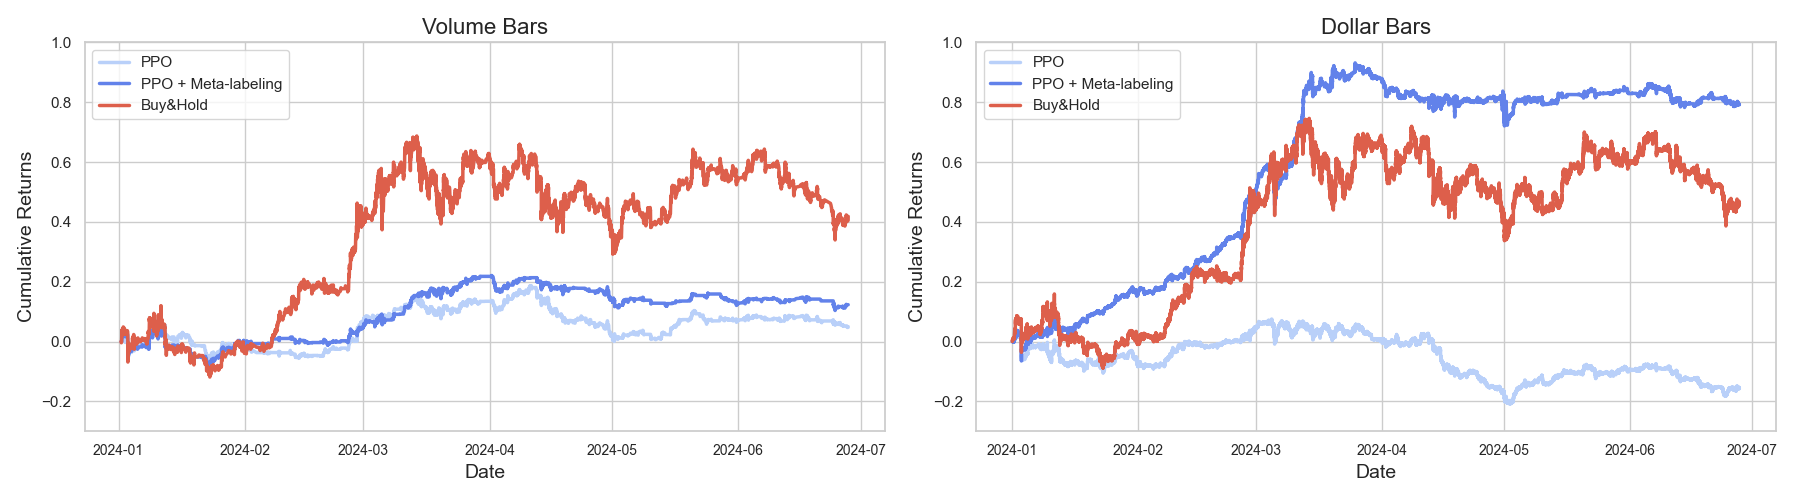
\includegraphics[width=1.05\textwidth]{./figures/final_btc_strategy_comparison_horizontal.png}
        \caption{Comparativa de retornos acumulados de la estrategia final sobre BTC}
        \label{fig:final_btc_cum_returns_comparison_img}
    \end{figure}

    % \begin{table}[h]
    %     \centering
    %     \begin{scriptsize}
    %     \begin{tabular}{|>{\scriptsize\centering\arraybackslash}m{4cm}|c|c|c|c|c|c|c|c|c|}
    %     \hline
    %     & \makecell{\textbf{Cumulative} \\ \textbf{Returns}} & \makecell{\textbf{Annualized} \\ \textbf{Return}} & \makecell{\textbf{Sharpe} \\ \textbf{Ratio}} & \makecell{\textbf{Sortino} \\ \textbf{Ratio}} & \makecell{\textbf{Maximum} \\ \textbf{Drawdown}} & \makecell{\textbf{Calmar} \\ \textbf{Ratio}} & \makecell{\textbf{Value at} \\ \textbf{Risk (VaR)}} & \textbf{Alpha} & \textbf{Beta} \\ \hline
    %     \makecell{\textbf{Benchmark} \\ \textbf{(BTC)}} & 0.418 & 0.640 & \textbf{0.160} & \textbf{0.224} & -0.234 & 2.734 & -0.006 & 0.000 & 1.000 \\ \hline
    %     \makecell{\textbf{PPO Volume} \\ \textbf{Bars}} & 0.050 & 0.071 & 0.055 & 0.075 & -0.156 & 0.455 & -0.003 & -0.001 & 0.274 \\ \hline
    %     \makecell{\textbf{PPO + Meta-labeling} \\ \textbf{Volume Bars}} & 0.123 & 0.178 & 0.121 & 0.168 & -0.149 & 1.200 & -0.002 & 0.001 & 0.226 \\ \hline
    %     \makecell{\textbf{PPO Dollar} \\ \textbf{Bars}} & -0.156 & -0.213 & -0.026 & -0.036 & -0.263 & -0.809 & -0.001 & -0.000 & 0.347 \\ \hline
    %     \makecell{\textbf{PPO + Meta-labeling} \\ \textbf{Dollar Bars}} & \textbf{0.792} & \textbf{1.283} & 0.125 & 0.176 & -0.109 & 11.760 & -0.001 & 0.001 & 0.230 \\ \hline
    %     \end{tabular}
    %     \caption{Resultados del rendimiento acumulado y métricas de riesgo para PPO con y sin \textit{Meta-labeling}, comparados con el Benchmark (BTC).}
    %     \label{tab:final_btc_cum_returns_comparison_table}
    %     \end{scriptsize}
    % \end{table}
  
    \begin{table}[h]
        \centering
        \begin{scriptsize}
        \begin{tabular}{|>{\scriptsize\centering\arraybackslash}m{5cm}|c|c|c|c|c|c|c|c|c|}
        \hline
        & \makecell{\textbf{Cumulative} \\ \textbf{Returns}} & \makecell{\textbf{Annualized} \\ \textbf{Return}} & \makecell{\textbf{Sharpe} \\ \textbf{Ratio}} & \makecell{\textbf{Sortino} \\ \textbf{Ratio}} & \makecell{\textbf{Maximum} \\ \textbf{Drawdown}} & \makecell{\textbf{Calmar} \\ \textbf{Ratio}} & \textbf{Alpha} & \textbf{Beta} \\ \hline
        \makecell{\textbf{Benchmark} \\ \textbf{(BTC)}} & 0.418 & 0.640 & \textbf{0.160} & \textbf{0.224} & -0.234 & 2.734 & 0.000 & 1.000 \\ \hline
        \makecell{\textbf{PPO Volume} \\ \textbf{Bars}} & 0.050 & 0.071 & 0.055 & 0.075 & -0.156 & 0.455 & -0.001 & 0.274 \\ \hline
        \makecell{\textbf{PPO + Meta-labeling} \\ \textbf{Volume Bars}} & 0.123 & 0.178 & 0.121 & 0.168 & -0.149 & 1.200 & 0.001 & 0.226 \\ \hline
        \makecell{\textbf{PPO Dollar} \\ \textbf{Bars}} & -0.156 & -0.213 & -0.026 & -0.036 & -0.263 & -0.809 & -0.000 & 0.347 \\ \hline
        \makecell{\textbf{PPO + Meta-labeling} \\ \textbf{Dollar Bars}} & \textbf{0.792} & \textbf{1.283} & 0.125 & 0.176 & -0.109 & 11.760 & 0.001 & 0.230 \\ \hline
        \end{tabular}
        \caption{Resultados del rendimiento acumulado y métricas de riesgo para PPO con y sin \textit{Meta-labeling}, comparados con el Benchmark (BTC).}
        \label{tab:final_btc_cum_returns_comparison_table}
        \end{scriptsize}
    \end{table}
    
  
\end{uselscape}





\begin{table}[h!]
    \centering
    \begin{tabular}{lccc}
    \hline
    \textbf{Conjunto de Datos} & \textbf{Benchmark} & \textbf{Rendimiento Antes} & \textbf{Rendimiento Después} \\
    \hline
    BTC Dollar  & 41.8\% & -15.6\% & 79.2\% \\
    BTC Volume  & 41.8\% & 5.0\% & 12.3\% \\
    SPY Original  & 14.6\% & 1.5\% & 9.6\% \\
    SPY Volume  & 14.6\% & 8.1\% & 7.6\% \\
    SPY Dollar  & 14.6\% & 7.3\% & 7.4\% \\
    \hline
    \end{tabular}
    \caption{Rendimiento acumulado final de las estrategias antes y después de aplicar \textit{meta-labeling}, comparado con el Benchmark.}
    \label{tab:final_returns_comparison}
\end{table}
    

Los resultados obtenidos muestran un panorama mixto en cuanto a la efectividad del \textit{meta-labeling}. 
Por un lado, las métricas de precisión y \textit{recall} han experimentado un deterioro tras la aplicación 
del \textit{meta-labeling}, lo que sugiere que el modelo filtrado se volvió más conservador, identificando 
menos señales de trading que el modelo original. Sin embargo, y a pesar de esta aparente desventaja, el 
rendimiento acumulado de la mayoría de las estrategias mejoró de manera significativa, con algunas 
estrategias mostrando incrementos notables en su rentabilidad.

Este fenómeno puede explicarse por la capacidad del \textit{meta-labeling} para reducir la exposición 
a operaciones fallidas, incluso si esto implica la pérdida de algunas operaciones exitosas. Al aplicar 
un filtro adicional a las señales generadas por el modelo primario, el \textit{meta-labeling} tiende a 
evitar operaciones en escenarios de mayor incertidumbre o cuando las señales no son lo suficientemente 
sólidas. Como resultado, aunque el número total de operaciones disminuye, las operaciones que se llevan 
a cabo son, en promedio, más rentables. Esto se refleja en el rendimiento acumulado de las estrategias, 
que mejora incluso en aquellos casos donde las métricas tradicionales de clasificación sugieren un 
empeoramiento.

En particular, las estrategias basadas en BTC Dollar y BTC Volume experimentaron mejoras destacables 
en su rendimiento acumulado después de aplicar \textit{meta-labeling}, con BTC Dollar mostrando un 
incremento sustancial que supera el rendimiento del Benchmark. Esto indica que el \textit{meta-labeling} 
puede ser especialmente útil en mercados volátiles como el de las criptomonedas, donde las señales de 
trading pueden ser más erráticas y el riesgo de operaciones fallidas es mayor. En este contexto, el 
\textit{meta-labeling} actúa como una capa adicional de protección, seleccionando solo las señales 
que pasan un filtro más estricto.

Por otro lado, las estrategias basadas en el S\&P 500 también mostraron mejoras, aunque más modestas, 
en su rendimiento acumulado. La menor volatilidad inherente al mercado de acciones podría explicar 
por qué el impacto del \textit{meta-labeling} no es tan pronunciado en comparación con los mercados 
de criptomonedas. Aun así, el hecho de que se observe una mejora, aunque ligera, sugiere que el 
\textit{meta-labeling} sigue siendo una herramienta valiosa para filtrar señales en contextos 
de menor volatilidad.

En resumen, aunque el \textit{meta-labeling} ha mostrado un impacto negativo en las métricas 
de precisión y \textit{recall}, su efecto global en las estrategias ha sido positivo, 
mejorando el rendimiento acumulado de manera significativa. Este hallazgo subraya la 
importancia de considerar el rendimiento global de una estrategia de trading, más allá de 
las métricas individuales de clasificación. El \textit{meta-labeling} se presenta como una 
metodología que, a pesar de su conservadurismo, logra incrementar la rentabilidad al priorizar 
la calidad sobre la cantidad de las operaciones ejecutadas.


\chapter{Conclusiones}

\section{Resumen de los Hallazgos Principales}


Este trabajo ha explorado la implementación de técnicas avanzadas de \textit{machine learning} 
en el desarrollo de estrategias de trading, con un enfoque particular en la aplicación de 
\textit{deep reinforcement learning} (DRL) para la generación de señales de trading. Además, 
se han adoptado metodologías presentadas en el libro \textit{Advances in Financial Machine Learning} 
de Marcos López de Prado, como las barras de desequilibrio y el \textit{Meta-Labeling}, para 
la generación de estas estrategias.

Inicialmente, se implementaron y compararon diferentes tipos de representaciones del mercado, 
como las barras de tiempo tradicionales frente a las barras de desequilibrio de volumen y dólares. 
Estas técnicas pretenden capturar la dinámica subyacente del mercado de manera más precisa al 
basarse en la actividad real en lugar de intervalos de tiempo fijos. Posteriormente, se 
utilizó el algorigítmo \textit{PPO} para entrenar un modelo de generación de señales de trading sobre estos distintos 
tipos de barras, evaluando cómo la representación del mercado afecta al rendimiento del modelo.

Finalmente, se aplicó la técnica de \textit{Meta-Labeling} para refinar las señales generadas por el 
modelo \textit{PPO}. Esta técnica agregó una capa adicional de análisis, mejorando la 
capacidad del modelo para identificar las señales de trading más prometedoras. 

Los resultados obtenidos muestran que, aunque la implementación del \textit{Meta-Labeling} 
no siempre mejoró las métricas de precisión y \textit{recall}, en muchos casos llevó a un 
aumento notable en el rendimiento acumulado de las estrategias. Esto sugiere que el 
\textit{Meta-Labeling} puede actuar como un filtro eficaz para mejorar la calidad de las 
operaciones ejecutadas, especialmente en mercados con alta volatilidad como el de las 
criptomonedas.


En conclusión, la combinación del \textit{deep reinforcement learning} con las metodologías 
propuestas en \textit{Advances in Financial Machine Learning} proporciona un enfoque 
potencialmente eficaz para la generación de estrategias de trading, aunque su rendimiento no se 
manifiesta uniformemente en todos los mercados, activos o condiciones. Si bien estas 
técnicas se han mostrado útiles como herramientas para el desarrollo de estrategias, 
su implementación es compleja y requiere un diseño cuidadoso, ya que la optimización es 
muy sensible a los hiperparámetros para obtener resultados satisfactorios. Esto sugiere que, 
aunque prometedoras, estas metodologías demandan un enfoque riguroso y específico para 
poder aprovechar plenamente su potencial en la práctica.


El código desarrollado para implementar las estrategias de \textit{Deep Reinforcement Learning} 
y las técnicas mencionadas en este trabajo, como las barras de desequilibrio y el \textit{Meta-Labeling}, 
está disponible públicamente para su revisión y uso en el 
siguiente repositorio de GitHub: \url{https://github.com/alexdlp/math_tfm}. 

En dicho repositorio se pueden encontrar las implementaciones completas, así como los 
experimentos realizados para validar el desempeño de las estrategias de trading algorítmico.


\section{Cumplimiento de los Objetivos}

Los objetivos planteados al inicio de este trabajo se han cumplido en gran medida. En 
primer lugar, se ha logrado desarrollar y evaluar una estrategia de trading utilizando 
técnicas avanzadas como las barras de desequilibrio, el \textit{deep reinforcement learning}, 
y el \textit{Meta-Labeling}. Estos esfuerzos han resultado en una comprensión más profunda 
de cómo estas herramientas pueden integrarse para mejorar el rendimiento de las estrategias 
de trading.

Además, se ha aprendido a implementar y ajustar algoritmos de \textit{deep reinforcement learning}, 
aprovechando librerías como \textit{Gymnasium} y \textit{Stable Baselines}. A través de la 
comparación de diferentes enfoques, se ha demostrado que el uso de barras de desequilibrio 
y \textit{Meta-Labeling} puede proporcionar ventajas significativas en ciertos contextos. 
Aunque se encontraron desafíos en la implementación, especialmente en términos de ajuste 
y optimización, el proceso ha sido valioso para adquirir habilidades prácticas en el 
uso de estas metodologías.

Finalmente, la comparativa entre técnicas ha revelado insights importantes sobre su 
efectividad y sus limitaciones. Los resultados obtenidos sugieren que, aunque cada 
técnica tiene sus propios méritos, la combinación de barras de desequilibrio y 
\textit{Meta-Labeling} ofrece un enfoque prometedor para desarrollar estrategias de 
trading más adaptativas y precisas.


\section{Limitaciones del Estudio}

A lo largo de este trabajo se han identificado varias limitaciones que afectan tanto a 
la implementación como a la generalización de los resultados obtenidos. Una de las 
principales limitaciones ha sido la accesibilidad y disponibilidad de datos de calidad. 
Los datos de ticks, que ofrecen una visión detallada del mercado, son costosos y difíciles 
de manejar debido a su tamaño y complejidad. Esto ha llevado a la utilización de datos de
 minuto, lo cual, aunque más manejable, puede no capturar completamente las sutilezas de 
 las dinámicas del mercado que los datos de ticks sí podrían reflejar.

Otra limitación significativa es la necesidad de un poder computacional considerable. El 
entrenamiento y la inferencia con algoritmos de \textit{deep reinforcement learning} 
requieren recursos computacionales extensivos. En muchas ocasiones, el tiempo necesario 
para entrenar modelos complejos es prohibitivo, y, aun disponiendo de tiempo suficiente, 
la infraestructura computacional limitada puede impedir la obtención de resultados óptimos. 
Este desafío se acentúa al intentar aplicar estos modelos a datos de alta frecuencia o 
grandes volúmenes de datos históricos.

Otra limitación importante es la generalización de los resultados. Los experimentos 
realizados en este estudio se basaron en datos específicos y en un conjunto limitado de 
escenarios de mercado. Por lo tanto, los resultados obtenidos pueden no ser directamente 
aplicables a otros mercados o condiciones sin una adecuada recalibración de los modelos. 
Esto limita la aplicabilidad de las estrategias desarrolladas, ya que lo que funciona bien 
en un contexto específico puede no ser efectivo en otro sin ajustes significativos.

La sensibilidad a los hiperparámetros y al diseño del modelo también representa una 
limitación crucial. Tanto la configuración de la función de recompensa como el diseño
 del entorno de trading pueden influir significativamente en el rendimiento de las 
 estrategias. La optimización de estos aspectos es un proceso delicado y sensible, 
 donde pequeños cambios en los hiperparámetros pueden llevar a variaciones considerables 
 en los resultados. Esto subraya la necesidad de un enfoque riguroso en la fase de diseño
  y ajuste de los modelos.

Finalmente, es importante destacar que el enfoque adoptado en este trabajo también enfrenta 
limitaciones en cuanto a la escalabilidad. La capacidad de aplicar las metodologías 
desarrolladas en este estudio a volúmenes de datos mucho mayores o a mercados diferentes 
sin una recalibración exhaustiva de los modelos es cuestionable. La adaptabilidad de los 
algoritmos a nuevos datos o condiciones de mercado requiere una flexibilidad en el diseño 
que puede no estar presente en los modelos actuales, lo que podría limitar su efectividad 
en entornos reales más diversos.

En resumen, aunque este trabajo ha demostrado el potencial de las metodologías utilizadas, 
es esencial tener en cuenta estas limitaciones al considerar la aplicabilidad y 
generalización de los resultados. Las futuras investigaciones deberán abordar estos 
desafíos para mejorar la robustez y la adaptabilidad de las estrategias de trading basadas 
en \textit{machine learning}.



\section{Implicaciones Prácticas}

Los resultados de este estudio tienen importantes implicaciones prácticas para el desarrollo 
y la implementación de estrategias de trading en entornos financieros. En primer lugar, la 
aplicación de \textit{deep reinforcement learning} (DRL) junto con metodologías avanzadas 
como las barras de desequilibrio y el \textit{Meta-Labeling}, propuestas en \textit{Advances 
in Financial Machine Learning}, ofrece un enfoque innovador para la generación de estrategias de trading que pueden adaptarse dinámicamente a las condiciones cambiantes del mercado.

Uno de los principales beneficios de estas técnicas es su capacidad para capturar dinámicas 
de mercado más complejas y detalladas en comparación con los enfoques tradicionales basados 
en barras de tiempo. Las barras de desequilibrio de volumen y dólares, al basarse en la actividad 
real del mercado, permiten un análisis más fino de la oferta y la demanda, lo que puede mejorar 
la precisión en la identificación de oportunidades de trading. Esto es especialmente relevante 
en mercados volátiles, como el de criptomonedas, donde las señales de trading pueden ser más 
erráticas y difíciles de interpretar utilizando metodologías tradicionales.

Sin embargo, la implementación práctica de estas técnicas no está exenta de desafíos. El 
poder computacional requerido para entrenar y ejecutar modelos de DRL es considerable, 
lo que puede limitar su uso en entornos con recursos computacionales limitados. Además, 
la necesidad de datos de alta calidad, como los datos de ticks, que son costosos y 
difíciles de manejar, puede representar una barrera significativa para muchos actores 
del mercado. Esto sugiere que, aunque prometedoras, estas metodologías requieren una 
infraestructura tecnológica robusta y acceso a recursos que no siempre están disponibles.

Otro aspecto crítico es la sensibilidad de estas técnicas a los hiperparámetros y al 
diseño del entorno de trading. La optimización de los modelos y la calibración adecuada 
de los hiperparámetros son esenciales para obtener resultados consistentes y rentables. 
En la práctica, esto significa que los profesionales que buscan implementar estas 
metodologías deben estar preparados para invertir tiempo y recursos en la fase de 
experimentación y ajuste de los modelos.

A pesar de estos desafíos, las técnicas presentadas en este estudio ofrecen un marco 
valioso para el desarrollo de estrategias de trading más adaptativas y potencialmente 
más rentables. En particular, la capacidad del \textit{Meta-Labeling} para mejorar la 
calidad de las señales de trading y reducir la exposición a operaciones fallidas puede 
ser especialmente útil para gestores de fondos y traders que buscan maximizar el rendimiento 
mientras minimizan el riesgo.

En conclusión, aunque la implementación práctica de las técnicas desarrolladas en este 
estudio presenta desafíos significativos, sus beneficios potenciales las convierten en 
herramientas atractivas para aquellos que buscan innovar en el campo del trading algorítmico. 
Es esencial que los profesionales consideren cuidadosamente los requisitos técnicos y de 
datos antes de adoptar estas metodologías, y que estén preparados para un proceso de 
desarrollo y optimización riguroso.

\section{Líneas Futuras de Investigación}

A partir de los resultados y las limitaciones identificadas en este estudio, surgen 
varias líneas futuras de investigación que podrían contribuir a mejorar y ampliar el 
conocimiento en el campo del trading algorítmico basado en \textit{machine learning}.

% Una dirección importante para futuras investigaciones es la exploración de métodos 
% para mejorar la accesibilidad y el manejo de datos de alta frecuencia, como los datos 
% de ticks. Dado que estos datos ofrecen una representación más detallada del mercado, 
% el desarrollo de técnicas eficientes de procesamiento y análisis que puedan manejar 
% grandes volúmenes de datos de manera más efectiva podría abrir nuevas posibilidades 
% para el diseño de estrategias de trading más precisas y adaptativas.

En primer lugar, una de las principales áreas de interés es la exploración de otros algoritmos de 
aprendizaje por refuerzo, especialmente aquellos diseñados para espacios de acciónes continuos, como el 
\textit{Deep Deterministic Policy Gradient} (DDPG) o el \textit{Soft Actor-Critic} (SAC). Estos enfoques 
son particularmente útiles en mercados financieros, donde las decisiones de trading no se limitan a acciones 
discretas como comprar o vender, sino que pueden implicar ajustes graduales y continuos en las posiciones. 
El uso de estos algoritmos podría permitir una mayor flexibilidad en las estrategias de trading, adaptándose 
de manera más precisa a los cambios dinámicos en los mercados.

En este contexto, otro área de interés es el desarrollo de funciones de recompenssa 
que no solo optimicen el rendimiento total de la estrategia, sino que también tengán en cuenta el riesgo, 
mediante métricas como el \textit{Sharpe Ratio} o el \textit{Sortino Ratio}. Al introducir este tipo de 
funciones de recompensa, los modelos de aprendizaje por refuerzo podrían ser entrenados no solo para 
maximizar las ganancias, sino también para gestionar mejor el riesgo inherente a las operaciones. Este 
enfoque ayudaría a reducir la volatilidad del portafolio y mejoraría la estabilidad de las estrategias 
en diferentes condiciones de mercado.

Además, la generalización de los resultados a otros mercados y condiciones de mercado también 
representa una línea de investigación crítica. Futuras investigaciones podrían enfocarse 
en evaluar cómo las metodologías utilizadas en este estudio se desempeñan en diferentes 
mercados financieros, como el forex, los commodities o incluso mercados emergentes. Además, 
la exploración de diferentes horizontes temporales y escenarios de volatilidad podría 
ofrecer una mejor comprensión de las condiciones bajo las cuales estas metodologías son 
más efectivas.


Otra área de investigación prometedora es el desarrollo de enfoques más robustos para 
la optimización de hiperparámetros y el diseño de modelos. Dado que la sensibilidad a 
los hiperparámetros es una limitación significativa en la implementación de modelos de 
\textit{deep reinforcement learning} y \textit{Meta-Labeling}, se podrían explorar 
técnicas automatizadas de optimización de hiperparámetros, como \textit{hyperparameter tuning} 
basado en algoritmos genéticos o \textit{Bayesian optimization}, que podrían mejorar la 
eficiencia y efectividad del proceso de ajuste de modelos.


Asimismo, sería beneficioso explorar técnicas más avanzadas de gestión del riesgo y \textit{position sizing}. 
Métodos basados en la volatilidad o reglas adaptativas de asignación de capital podrían integrarse en los 
algoritmos de trading para ajustar el tamaño de las posiciones en función de la incertidumbre del mercado. 
Esta adaptación dinámica permitiría a los modelos reducir el tamaño de las posiciones en periodos de 
alta volatilidad y aumentarlas en situaciones de mayor estabilidad, optimizando así la relación riesgo/recompensa.

% Además, una línea de investigación con gran potencial es la incorporación de información macroeconómica y fundamental 
% en los modelos de aprendizaje por refuerzo. Actualmente, muchas de las estrategias basadas en DRL se 
% entrenan principalmente con datos de series temporales de precios y volúmenes, pero la inclusión de indicadores 
% macroeconómicos, datos de sentimiento del mercado o análisis fundamental podría mejorar significativamente la 
% capacidad de los modelos para anticipar tendencias y cambios en las condiciones del mercado. Por ejemplo, 
% variables como tasas de interés, datos de empleo o informes de beneficios corporativos podrían ayudar a que 
% las estrategias sean más robustas y predictivas frente a eventos externos.

Finalmente, dado el avance continuo de la infraestructura tecnológica, futuras 
investigaciones podrían explorar el uso de tecnologías como \textit{cloud computing} 
y \textit{distributed computing} para superar las limitaciones computacionales que 
actualmente restringen la implementación de modelos más complejos y la experimentación 
con volúmenes de datos más grandes. El aprovechamiento de estas tecnologías podría 
permitir una exploración más exhaustiva de diferentes configuraciones de modelos y 
ampliar el alcance de las aplicaciones de \textit{machine learning} en el trading algorítmico.

En conjunto, estas líneas futuras de investigación tienen el potencial de mejorar 
significativamente la eficacia y la aplicabilidad de las estrategias de trading basadas 
en \textit{machine learning}, y de abordar algunas de las limitaciones identificadas 
en el presente estudio.

%\phantomsection
%\addcontentsline{toc}{chapter}{BIBLIOGRAFIA}
\bibliographystyle{plain}
\bibliography{biblioTFM}

\end{document}